\documentclass[fontsize=11pt,paper=a4,pagesize=auto,parskip=half-]{scrbook}
\usepackage{scrhack}
% ---------------------------
% Encoding, fonts, language
% ---------------------------
\usepackage[utf8]{inputenc}
\usepackage[T1]{fontenc}
\usepackage{amsmath}
\usepackage{mathpazo}\linespread{1.05}
\addtokomafont{disposition}{\rmfamily}
\usepackage[english]{babel}
\usepackage[expansion=false]{microtype}
\usepackage{csquotes}
\frenchspacing
% ---------------------------
% Bibliography
% ---------------------------
\usepackage{lettrine}
\usepackage{caption}
\captionsetup{format=plain, font=small, labelfont=bf}
\usepackage{imakeidx}
\makeindex[intoc=true, title={Index}]
% Niels's house index macros (from sr-good.sty): \Ix lowercases the key so
% capitalised and lowercase uses of a term sort as one entry; \Iy for persons.
\newcommand{\Ixtmp}{}
\DeclareRobustCommand{\Ix}[1]{%
  #1%
  \begingroup
    \lowercase{\gdef\Ixtmp{#1}}%
    \expandafter\index\expandafter{\Ixtmp}%
  \endgroup}
\newcommand{\Iy}[1]{#1\index{#1}}
\emergencystretch=3em
% ---- digital vs print edition: colored links on screen, black in print ----
\newif\ifdigitaledition
\digitaleditiontrue   % flip to \digitaleditionfalse for the print interior
\usepackage{xcolor}
\usepackage{hyperref}
\usepackage{hyperxmp}
% link triad shared with Synthesized Roots (TeBlue / FePurple / SeRed)
\definecolor{bbulink}{RGB}{0,76,153}
\definecolor{bbucite}{RGB}{128,0,128}
\definecolor{bbuurl}{RGB}{200,0,0}
% ---- figure accent palette: three accents at staggered luminance, so the
% ---- grayscale interior keeps every distinction. blue = momentum/gravity/waves,
% ---- red = energy/heat/repulsion, gold = light/depletion/counting.
\ifdigitaledition
  \hypersetup{colorlinks=true, linkcolor=bbulink, citecolor=bbucite, urlcolor=bbuurl}
  \definecolor{bbuBlue}{HTML}{2E5A78}
  \definecolor{bbuRed}{HTML}{B3432B}
  \definecolor{bbuGold}{HTML}{C08A2D}
\else
  \hypersetup{hidelinks}
  \definecolor{bbuBlue}{gray}{0.22}
  \definecolor{bbuRed}{gray}{0.42}
  \definecolor{bbuGold}{gray}{0.60}
\fi
\hypersetup{
  pdfauthor    = {Niels Bonde Jensen},
  pdftitle     = {The Billiard Ball Universe: A World With No Bottom},
  pdfsubject   = {Draft version},
  pdfkeywords  = {cosmology, philosophy of physics, infinite regress, Le Sage gravity, mechanical philosophy, infinite universe, ethics of infinity},
  pdfcopyright = {Copyright (C) 2026 by Niels Bonde Jensen. All rights reserved.}
}
\usepackage[capitalize,nameinlink]{cleveref}
\usepackage[backend=biber,style=numeric,sorting=nyt]{biblatex}
\addbibresource{ref.bib}
% ---------------------------
% Page: 6in x 9in trade book, single column
% ---------------------------
\usepackage{geometry}
\geometry{
  paperwidth=6in, paperheight=9in,
  inner=0.85in,
  outer=0.65in,
  top=0.75in, bottom=0.85in
}
\emergencystretch=3em
\hbadness=8000
\vbadness=8000
% ---------------------------
% Colors, symbols
% ---------------------------
\usepackage[dvipsnames]{xcolor}
\definecolor{TeBlue}{RGB}{0,76,153}
\definecolor{FePurple}{RGB}{128,0,128}
\definecolor{SeRed}{RGB}{200,0,0}
\usepackage{pifont}
\usepackage{graphicx}
\usepackage{tikz}
\usepackage{flafter}
\renewcommand{\topfraction}{0.9}
\renewcommand{\bottomfraction}{0.6}
\renewcommand{\textfraction}{0.07}
\renewcommand{\floatpagefraction}{0.85}
\setcounter{topnumber}{3}
\setcounter{totalnumber}{5}
\usepackage{booktabs}
\usepackage{ifthen}
\usepackage{array}
\newcolumntype{P}[1]{>{\raggedright\arraybackslash}p{#1}}
\usetikzlibrary{calc}
% Visual separator (house style)
\newcommand\En{\centerline{\textemdash \qquad \ding{166} \qquad \textemdash}}
\newcommand\End{\ding{166}}
% Chapter-opener art (engraving-style illustrations in art/)
\newcommand{\chapterart}[1]{%
  \begin{center}\includegraphics[width=0.62\textwidth]{art/#1}\end{center}\vspace{0.5em}}
% ---------------------------
% Dialogue and draft apparatus
% ---------------------------
\newcommand{\speaker}[1]{\par\noindent\textbf{#1:}\hspace{0.6em}}
\newif\ifdraftnotes
\draftnotestrue   % set \draftnotesfalse for a clean reading copy
\newenvironment{draftnote}{%
  \ifdraftnotes\par\small\itshape\color{black!60}\noindent[Craft notes: \ignorespaces
  \else\setbox0\vbox\bgroup\fi}{%
  \ifdraftnotes]\par\normalcolor\normalsize
  \else\egroup\fi}
\newcommand{\draftstatus}[1]{\ifdraftnotes{\small\itshape\color{black!60}#1\par}\fi\medskip}
% Sections unnumbered (trade-book style), chapters numbered
\setcounter{secnumdepth}{0}
\setcounter{tocdepth}{1}
% ---------------------------
% Metadata + hyperref
% ---------------------------
\usepackage{hyperref}
\usepackage{hyperxmp}
\hypersetup{
  pdfauthor   = {Niels Bonde Jensen},
  pdftitle    = {The Billiard Ball Universe: A World With No Bottom},
  pdfsubject  = {Draft version},
  pdfkeywords = {infinite regress, mechanical philosophy, Le Sage gravity, relational space, multiverse, infinite copies, ethics, grounding, metaphysics},
  pdfproducer = {TeX version},
  pdfcreator  = {LaTeX editor},
  pdfcopyright= {Copyright (C) 2026 by Niels Bonde Jensen. All rights reserved.},
  colorlinks  = true,
  linkcolor   = TeBlue,
  citecolor   = FePurple,
  urlcolor    = SeRed
}
\begin{document}
% ---------------------------
% Title page
% ---------------------------
\begin{titlepage}
\centering
\vspace*{1.6in}
{\Huge\bfseries The Billiard Ball Universe\par}
\vspace{0.35in}
{\Large\itshape A World With No Bottom\par}
\vspace{1.2in}
{\large Niels Bonde Jensen\par}
\vfill
{\small Draft 1 --- \today\par}
\vspace*{0.5in}
\end{titlepage}
\frontmatter
\tableofcontents

\addchap{How to Read This Book}
This book is written for two readers at once: the physicist, and the interested layman who owns no physics. For the second reader, three helps are provided, and one promise. Footnotes decode a term of art the first time it appears --- briefly, and only to decode; the argument itself never hides in a footnote. Appendix~A is a small dictionary of every technical term the book leans on, physics and philosophy alike; when a footnote ends with \emph{(Dictionary)}, a fuller entry waits there. Appendix~B states, in a few pages and without argument, what mainstream physics actually claims --- the standard picture this book spends its later chapters arguing with; the reader who has never met that picture may want those pages before Chapter~6. The promise: everything essential is in the main text, in plain prose. The physicist may ignore the apparatus entirely; the layman may lean on it without missing anything the physicist gets.

\begin{center}
\textbf{A Note to the Reader}\\[0.45em]
\parbox{0.86\textwidth}{\centering This book blends established material with original ideas and interpretations. Some of its claims reflect my own perspective and differ from mainstream views --- and the text says which is which, every time. I invite you to read with curiosity and a healthy measure of critical thinking; nothing here asks to be believed on authority.}
\end{center}
\mainmatter
\part{The Demand}
\chapter{\emph{No Magic Anywhere}}
\chapterart{ch1_child_window}
\draftstatus{Draft 1 --- needs the author's real memories and corrections}

\lettrine{T}{wo} things felt wrong to me as a child. Not ``philosophically troubling.'' Wrong. Obviously wrong, the way it is obvious that someone is cheating at a game even before you can say which rule they broke.

The first was action-at-a-distance.

I was told that the Sun pulls on the Earth. Pulls it --- across a hundred and fifty million kilometers of nothing. No rope. No pushing. Nothing traveling from one to the other. The Sun is there, the Earth is here, and the force simply \emph{acts}, across all that emptiness, because... it does.

That is cheating. I felt it then and I will say it stronger now: it is clearly cheating. If one thing affects another thing, then \emph{something happens between them}. Something travels, something touches, something pushes. A billiard ball moves because another ball hit it. That is not naivety --- that is the minimum standard for an explanation. ``It pulls, from far away, through nothing'' is not an explanation. It is a description of the mystery wearing the costume of an answer.

I remember the pleasure --- real pleasure --- when I learned what light was. Because that explained \emph{seeing}. Something actually travels from the thing to your eye. The lamp, the light, the eye: a complete, honest chain, with no gap in it anywhere. Seeing was not magic; seeing was delivery. And I remember assuming, in the way a child assumes, that this was a requirement everyone shared --- that of course all people demanded an unbroken chain between cause and effect, and of course the adults were busy filling in the remaining chains. It took me years to discover that most people do not demand this at all. They will accept ``it pulls'' and move on. I could not, and I still cannot.

I learned much later that I was in good company. Newton --- the man who gave us this pulling-across-nothing --- privately agreed with the child I was. He wrote that the idea of one body acting on another through a vacuum, without anything mediating, was an absurdity that no competent thinker could accept. He built the most successful theory in the history of science on a mechanism he himself refused to believe in. The mathematics worked, and he declined to guess at the machinery underneath. Fair enough. But someone should keep looking for the machinery. This book is me looking.

Then came the second experience, and it was worse, because it arrived disguised as the cure.

Eventually one learns how modern physics ``fixed'' Newton's embarrassment: gravity is not a pull across space --- it is the \emph{curving of space itself}. The Sun bends the space around it, and the Earth simply follows the bent space. This is presented as the triumph over action-at-a-distance. And when I learned it, it felt extremely wrong. Not an improvement --- the same cheat, moved one step back and better hidden.

Because look at what is being claimed. Space is bent. Bent --- \emph{what}, exactly? Space is not a thing. Space is obviously nothing: it is not made of anything, you cannot push it, collect it, or take a piece of it away. Space is just the word for the relations between the actual things --- the actors. Where the actors are, and how they can move with respect to each other: \emph{that} is what space is, and all that it is. If the actors are three-dimensional objects, then space will appear three-dimensional, because space is nothing but the shape of their possibilities. So ``the Sun bends space'' means: the Sun acts on nothing, and the nothing then tells the Earth how to move. That is action-at-a-distance with an extra step and a mathematical costume. You do not escape the cheat by giving the gap between things a name and then bending the name.

I did not know then that this, too, was an old war, and that I had picked the same side as Leibniz, who told Newton to his face --- through letters --- that space is not a thing but an order of relations among things. The child's version and Leibniz's version are the same complaint: you cannot act on nothing, and you cannot make nothing do work in your explanation.

The second thing that felt wrong was borders.

Any time someone described a boundary of everything --- an edge of the universe, a smallest particle, a bottom layer of reality --- the same questions arrived immediately and would not leave. Who made the border? What is the border itself made of? What is inside the wall? And what is on the other side of it? A border does not close the questions. It multiplies them. Every edge someone proposed was just a place where they had decided to stop asking, and then painted the stopping-place to look like an answer.

I did not know, as a child, that a Roman poet had the same complaint two thousand years ago. Lucretius said: walk to the supposed edge of the universe and throw a spear. Either it flies onward --- and then there was no edge --- or something stops it, and then that something is beyond your ``edge,'' and there was no edge. Whichever way it goes, the border loses. A child can run that argument. I did, without knowing his name.

These two feelings are really one feeling. Action-at-a-distance is magic in the forces: influence with no mechanism. A final border --- an edge, a bottom, a smallest thing --- is magic in the structure: a level of reality that ``just is,'' with no reason, where you are instructed to stop asking. Both are the same move: at some point, the explanation stops, and you are told the stopping is fine.

I do not think the stopping is fine. I think a world can be demanded in which nothing acts without touching, and nothing exists without being made of something, and no level is allowed to be magic. Everything pushes. Everything is made of smaller things, which are made of smaller things, without end. All the way down, and all the way out.

Almost everyone I describe this to has the same reaction: an infinite regress explains nothing, you must ground out \emph{somewhere}. I spent a long time testing that objection, and the honest result of that testing is Chapter 3 --- it does not go the way either side expects. And the physics of how such a world might actually work --- particles, shadows, pushing --- is sketched later, along with the places where the sketch breaks, because it does break, in instructive places.

But the argument comes later. This chapter has only one job: to put the two childhood convictions on the table, undiluted, before any philosophy touches them.

No pulling through nothing. No border anyone painted. No magic anywhere.

The rest of the book is the price of taking that seriously.

\En

\begin{draftnote}
Author to add, if possible: rough ages for the two experiences (learning about light; learning about curved space), and any physical detail --- where you were, who explained it, a book or classroom. Even one sentence of real place per scene grounds the chapter. The border-intuition still has no concrete scene; if a memory exists, add it, but the chapter works without it.
\end{draftnote}

\chapter{\emph{The Old Tradition}}
\chapterart{ch2_spear_edge}
\draftstatus{Draft 1}

\lettrine{T}{he} convictions of Chapter 1 arrived, in me, as a child's certainties --- private, wordless, and, I assumed, universal. They are not universal. But they are also not mine. Everything this book demands has been demanded before, by a lineage of thinkers stretching back more than two thousand years, and this chapter is that genealogy. I tell it for two reasons. The first is honesty: a reader should know which of this book's ideas are old, and every one of its \emph{demands} is old; only some of its combinations are new. The second is instruction: the lineage is not a parade of ancestors to admire. It is a sequence of attempts, and each attempt \emph{failed in a specific, recorded way} --- and the failures are the most valuable inheritance of all. By the end of this chapter, the reader will know exactly which walls the tradition has already hit, so that when this book hits some of the same walls in Chapter 7, we will at least hit them with our eyes open.

\section{The Poet of Atoms}

Begin in Rome, around fifty years before Christ, with a poem --- six books of Latin verse called \emph{De Rerum Natura}, ``On the Nature of Things,'' by Titus Lucretius Carus, about whom almost nothing is known except that he wrote one of the most astonishing documents in the history of thought.

Lucretius was an Epicurean --- a follower of the Greek Epicurus, who was himself heir to Democritus, the first of all atomists. The picture the poem lays out, in verse, as physics, is this: everything is atoms and void. Unbreakable small bodies, moving, colliding, combining, in emptiness without limit. No hidden forces. No divine steering. Every phenomenon --- wind, magnetism, thought, the soul itself --- is atoms doing what atoms do: touching and pushing. It is, two millennia early, the billiard-ball universe, complete with its founding refusal: nothing acts but by contact.

And it contains the child's second conviction too, in the most famous thought-experiment of antiquity. Suppose, says Lucretius, the universe has a boundary~\cite{lucretius}. Walk to it. Now throw a spear at the edge. Either the spear flies onward --- in which case there was no boundary --- or something stops it --- in which case there is something beyond your ``boundary,'' and it was no boundary at all. Repeat at every claimed edge, forever. Space cannot end, because an end would have to have another side. When I made my child's version of this argument --- \emph{who built the border? what is behind the wall?} --- I was reinventing, badly, a Roman's verse. It is the oldest argument in this book, and I have never seen it answered; the modern escape (space that curves back on itself, finite but unbounded) does not answer the spear --- it changes the subject to a space that has no edge to throw over, which is, in its way, a concession.

\begin{figure}[p]\centering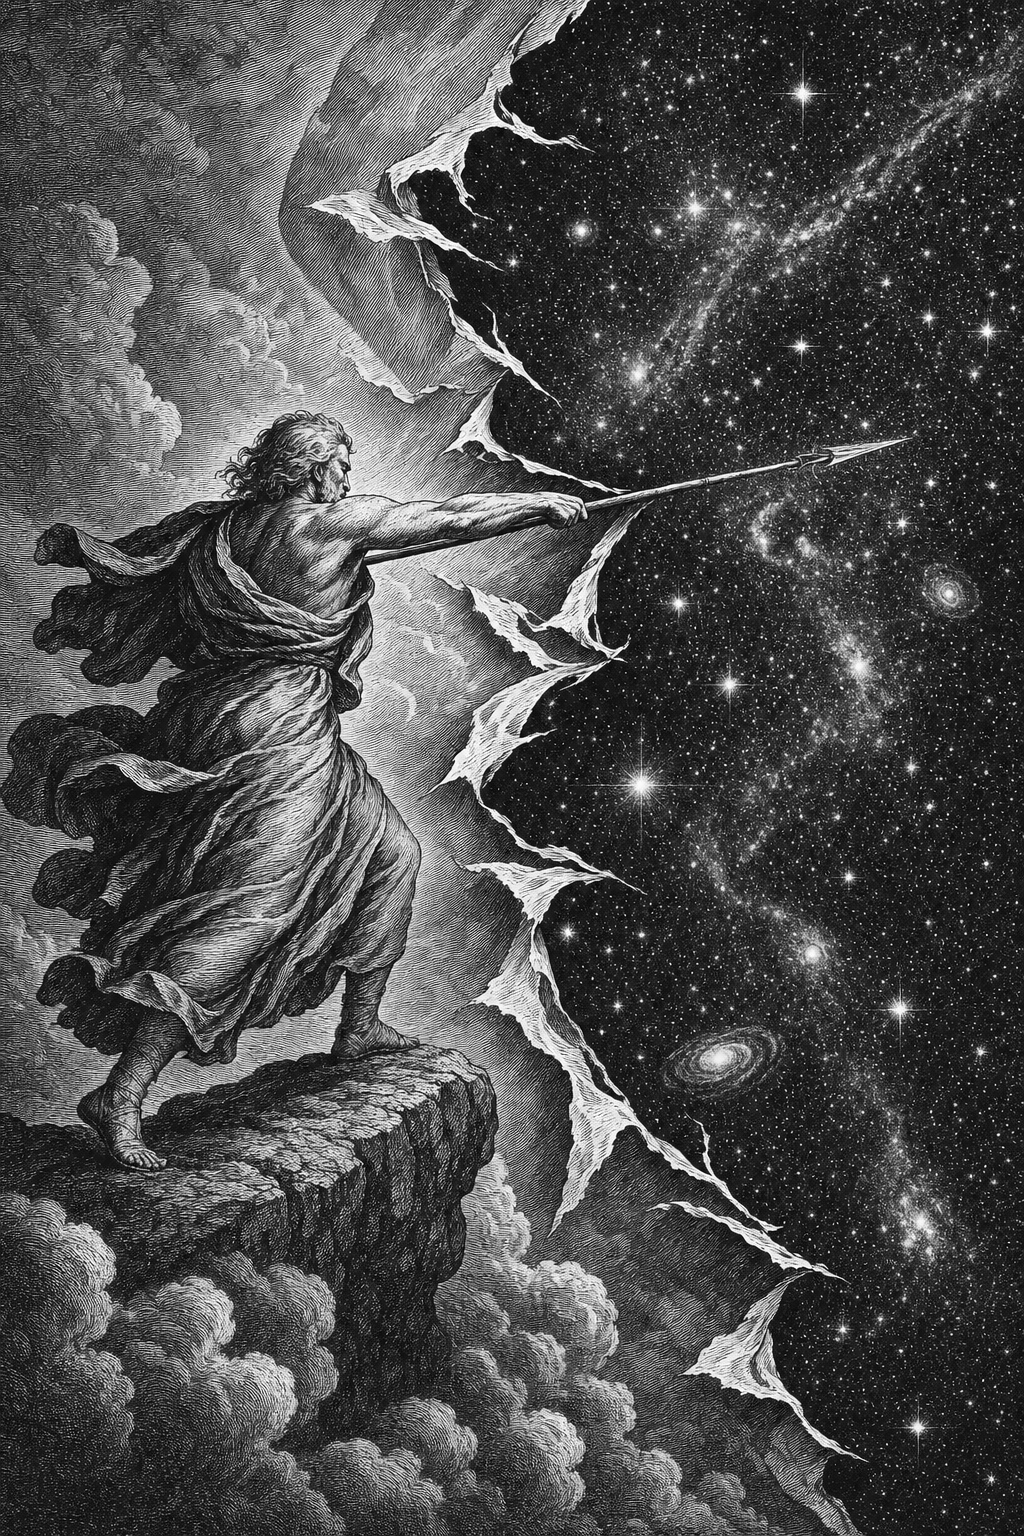
\includegraphics[height=0.92\textheight,width=\textwidth,keepaspectratio]{art/plate_spear_edge}\end{figure}

One more thing about Lucretius, because it anticipates Chapter 5 of this book by twenty centuries: his physics had a moral purpose. The poem's declared aim is the removal of two fears --- fear of the gods, and fear of death --- and both removals follow from the mechanics. A universe of atoms and void leaves no room for divine punishment; and death, being the dispersal of one's atoms, is the end of all experience and therefore of all harm: \emph{where death is, we are not.} From infinite worlds and mechanical nature, Lucretius drew conclusions about how to live and how to feel. A book that moves from billiard balls to ethics is not committing a genre error. It is resuming the original program.

\section{The Man Who Would Not Take It Back}

The poem was nearly lost --- it survived antiquity, by most accounts, in a whisper of copies, and was hauled back into circulation in 1417 by a book-hunting Italian secretary named Poggio Bracciolini~\cite{greenblatt2011,palmer2014}, after which it detonated slowly across Europe for two centuries. One of the places it detonated was the mind of Giordano Bruno.

Bruno, a Neapolitan ex-monk of spectacular arrogance and courage, took the infinite universe further than anyone had dared: not just infinite space, but infinite \emph{worlds}~\cite{bruno1584} --- the stars are suns, he said, and around them circle other earths, inhabited, without number, none of them the center, because an infinite universe has no center to be. He wandered Europe for two decades publishing this and much else, was lured back to Italy, and spent eight years in the prisons of the Inquisition, which demanded he recant a list of propositions. He would not --- the accounts we have suggest he told his judges that they pronounced sentence upon him with greater fear than he received it~\cite{rowland2008} --- and on the seventeenth of February, 1600, he was burned in Rome's Campo de' Fiori, where his statue now stands, hooded, facing the Vatican.

Honesty requires a complication: Bruno was condemned as a heretic on a docket that was mostly theology --- the infinite worlds were among the charges, but so were his views on considerably more ecclesiastical matters, and historians rightly resist the simple story of ``martyr for science.'' I keep him in the lineage anyway, and not for the martyrdom. I keep him for the \emph{direction} of his inference. Bruno reasoned that an infinite cause could not have made a finite world --- that limitlessness, once admitted anywhere, floods everything. It is the same inference this book makes about layers: once you concede there is no edge \emph{outward}, the concession travels, and there is no privileged scale, no chosen center, no reason for the flooding to stop at any border whatsoever. Bruno is the first person on record to feel the full vertigo of \emph{nothing is globally special} --- and, in his strange way, the first to insist it was good news.

\section{Machines All the Way}

Half a century later, the demand for contact became, briefly, the official program of European science. René Descartes --- whose physics is now remembered mostly as the thing Newton demolished --- proposed a universe with no void at all~\cite{descartes1644}: space \emph{stuffed} with matter, whirling in great vortices, planets carried around their suns like leaves in a whirlpool, every force a push, every push a contact. The details were wrong, essentially all of them. But the \emph{rule} Descartes enforced --- that an explanation must be a mechanism, that ``occult qualities'' (hidden powers acting mysteriously) were forbidden --- trained a generation. Christiaan Huygens, the greatest physicist between Galileo and Newton, held the rule absolutely: when Newton's gravity arrived, Huygens accepted the mathematics with admiration and rejected the pulling as a physical claim~\cite{huygens1690} --- an ``absurdity,'' he called it, essentially the same word the child in Chapter 1 used, and he demanded a mechanical cause behind the inverse square.\footnote{The inverse-square law: double the distance and the force falls to a quarter --- the observed shape of gravity and, later, of electric attraction. Chapter~6 derives it from the geometry of shadows.}

I want the reader to sit for a moment with how the seventeenth century saw this, because our era has it exactly reversed. Today, ``mechanical philosophy'' sounds naive and ``action at a distance'' sounds like sophisticated physics. To Descartes and Huygens --- and to Leibniz, and to Newton himself --- it was precisely the other way around: contact was the \emph{sober} position, the adult refusal of magic, and unmediated attraction was a relapse into the medieval occult, spirits and sympathies dressed in geometry. The mechanical philosophers were not failing to be modern. They were \emph{defining} what rigor meant, and by their definition, it is our textbooks that have gone soft.

\section{The Embarrassed Triumph}

Then came the \emph{Principia}, 1687, and the strangest episode in the lineage: the demand's greatest defeat, administered by a man who shared the demand.

Newton's law of universal gravitation worked as nothing in the history of thought had ever worked~\cite{newton1687} --- the tides, the moon, the planets, the comets, one formula, no exceptions. And the formula said: every mass attracts every mass, across any distance, through anything, instantly. Asked for the mechanism, Newton gave the most famous shrug in science --- \emph{hypotheses non fingo}, I feign no hypotheses --- and the shrug is usually told as serene confidence. It was not serene. In a letter to the young theologian Richard Bentley, Newton wrote the sentence I have already quoted once in this book and will now quote properly, because it is the hinge of the whole story: that one body should act upon another at a distance through a vacuum, without the mediation of anything else, ``is to me so great an absurdity that I believe no man who has in philosophical matters a competent faculty of thinking can ever fall into it.''~\cite{janiak2014} Gravity, he told Bentley, must be caused by an agent --- whether material or immaterial he left, carefully, to his readers.

Hold both halves of that in one hand: the man who gave the world action-at-a-distance regarded belief in action-at-a-distance as a mark of philosophical incompetence. The theory triumphed anyway --- triumph has a way of retiring questions without answering them --- and Europe gradually stopped asking what gravity \emph{is}, having learned so profitably what it \emph{does}. That is the settlement this book calls cheating, and it is worth being precise about who signed it: not Newton, who refused to; not Huygens or Leibniz, who protested it. Nobody signed it. It simply set in, the way a habit does, and three centuries later it is mistaken for a discovery.

\section{The Letters}

The protest, at least, got itself written down, in the most consequential exchange of letters in the history of philosophy of physics. In 1715 and 1716, Gottfried Wilhelm Leibniz --- Newton's rival in the invention of calculus and his superior in metaphysical nerve --- exchanged five rounds of letters with Samuel Clarke~\cite{leibnizclarke}, Newton's spokesman (with Newton, most scholars think, close behind the curtain). Among the battlefields was the nature of space itself. Newton's physics assumed absolute space: a vast, real, invisible container, existing whether or not anything is in it --- God's sensorium, Newton had ventured. Leibniz replied that this container is a phantom. Space, he argued, is nothing but the \emph{order of coexistence} --- the system of relations among things; take away the things and you have not emptied space, you have abolished it. His weapon was a principle this book's readers have already met in other clothes: nothing is so without a \emph{sufficient reason} why it is so and not otherwise. If absolute space existed, God would have had to place the world \emph{here} rather than three feet to the left --- two arrangements identical in every relation, differing in nothing observable --- a choice with no possible reason. A difference that makes no difference, Leibniz held, is no difference; and a space distinct from the ordering of its contents is exactly such a nothing.

The reader of Chapter 1 knows this argument. It is the child's --- \emph{space is obviously nothing; the actors define it} --- stated by the man who co-invented calculus. Leibniz died in 1716, mid-correspondence; officially, Newton's side carried the field, because Newton's physics worked and no relationalist physics existed. But the argument would not die. In the nineteenth century Ernst Mach revived it with a physicist's edge~\cite{mach1883} --- all motion is relative to the world's matter, and mechanics should mention nothing else --- and Mach's principle, famously, was lodestar to the young Einstein, who hoped general relativity would vindicate it. Here the story turns ironic in the exact way Chapter 1 experienced: the theory built partly to honor the relational instinct issued in a spacetime that bends, waves, and carries energy --- a participant so muscular that most physicists now speak of it as a \emph{thing} again. The lineage's deepest quarrel remains unsettled after three hundred years; this book has taken its side of it, and pays that side's costs in Chapter 7.

\section{The Shadow Men}

Which leaves the mechanism itself --- and the two men who tried to build honest gravity, whose attempt this book's Chapter 6 knowingly revives.

Nicolas Fatio de Duillier was a brilliant young Genevan mathematician, for some years the closest friend Newton had (their falling-out is its own sad story). In 1690 Fatio proposed~\cite{fatio1690}, to the Royal Society itself, the mechanism the reader has already seen: space streaming in every direction with minute swift corpuscles; bodies shading one another from the stream; gravity as the push of the unshaded remainder. Newton knew the theory well and --- this is remarkable, and Fatio boasted of it --- treated it as the \emph{only possible mechanical explanation} of gravity, though he inclined, himself, to leave the cause with God rather than corpuscles. Fatio's theory found no traction and its author drifted into religious enthusiasms and obscurity.

A half-century later, knowing of Fatio's work, another Genevan --- Georges-Louis Le Sage --- rebuilt the theory with lifelong stubbornness, publishing from the late 1740s onward and giving the stream its enduring name, \emph{ultramundane corpuscles}: particles from beyond the world. Le Sage grasped exactly what he was selling. He titled his mature exposition \emph{Lucrèce Newtonien}~\cite{lesage1782} --- ``The Newtonian Lucretius,'' 1782 --- the atomist's contact-only universe, upgraded until it yielded Newton's inverse square. For a century his theory was the standing answer to ``what would honest gravity look like?'', examined by the first rank of physics: Laplace probed what the finite speed of a gravitational stream would do to orbits~\cite{laplace1805}; Kelvin, in the 1870s, tried to save the mechanism by letting bodies re-emit what they absorbed~\cite{kelvin1873}; Maxwell weighed the whole scheme in the ninth \emph{Britannica} and reported, with regret, its thermal impossibility~\cite{maxwell1875}; Poincaré, decades later, closed the ledger with the arithmetic of drag and heat~\cite{poincare1908}. The pincer of Chapter 7 --- this book's first and worst wound --- is not a hazard I discovered. It is the recorded cause of death of the tradition's best attempt, and I have inherited the theory and its autopsy together. That is what it means to work in a lineage: the toy in Chapter 6 was built in full knowledge of where its ancestor is buried.

One more inheritance, closer to home. In 1820, in Copenhagen, Hans Christian Ørsted noticed a compass needle twitch beside a current-carrying wire~\cite{oersted1820}, and in following it discovered that electricity in motion wraps \emph{circulation} around itself --- the magnetic swirl, force running in circles about the wire. It was the first crack in the purely central-force picture of nature and the seed of everything electromagnetic; and I confess it pleases me, as a Dane, that the lineage's one experimental gift to this book's Chapter 6 --- the hint that nature's forces are built of circulations --- was found here, by a countryman, with a compass and a wire.

\section{The Shape of the Lineage}

Stand back, and the genealogy has a shape.


\begin{figure}[htbp]
\centering
\begin{tikzpicture}[>=stealth]
  \draw[->, line width=0.9pt] (-0.25,0) -- (10.15,0);
  \foreach \x/\pos/\yr/\who in {
    0.0/above/{c.~55 BC}/{Lucretius},
    0.88/below/{1417}/{Poggio},
    1.76/above/{1600}/{Bruno},
    2.64/below/{1644}/{Descartes},
    3.52/above/{1687}/{Newton},
    4.40/below/{1690}/{Fatio},
    5.28/above/{1715}/{Leibniz},
    6.16/below/{1782}/{Le Sage},
    7.04/above/{1820}/{\O rsted},
    7.92/below/{1870s}/{Kelvin, Maxwell},
    8.80/above/{1887}/{Michelson},
    9.68/below/{1908}/{Poincar\'e}} {
    \draw[line width=0.8pt] (\x,-0.09) -- (\x,0.09);
    \ifthenelse{\equal{\pos}{above}}{
      \node[anchor=south, align=center, text width=1.42cm, inner xsep=1pt] at (\x,0.16) {\scriptsize \yr\\[-3pt]\scriptsize \who};
    }{
      \node[anchor=north, align=center, text width=1.42cm, inner xsep=1pt] at (\x,-0.16) {\scriptsize \yr\\[-3pt]\scriptsize \who};
    }
  }
\end{tikzpicture}
\caption{The lineage, not to scale. A demand stated in verse in antiquity; nearly lost, recovered in 1417; costing a life in 1600; the official rigor of Europe by 1644; defeated by its own greatest heir in 1687 while he privately agreed with it; protested in the finest correspondence in the philosophy of physics; attempted honestly, twice, by two Genevans; handed one experimental gift in Copenhagen in 1820; and killed, fairly, by the arithmetic of the 1870s--1900s. The demand itself survived every one of its mechanisms.}
\label{fig:lineage}
\end{figure}

A demand is stated in antiquity, at full strength, in verse: contact only, no edges, and a way of living drawn from the physics. It is nearly lost, returns, and costs a man his life in a Roman square. It becomes, briefly, the official rigor of Europe --- then is defeated by its own greatest heir, whose theory works too well to reject and asserts what he himself calls an absurdity. The defeat is protested in the finest philosophical correspondence ever written; the protest loses on points and refuses to die. The mechanism is attempted honestly, twice, by two Genevans, and is killed --- fairly, by arithmetic --- in a pincer that still holds. And the demand, evicted from physics proper, survives where it began: as a conviction, arriving unbidden in children who have never heard of any of these men, that pulling through nothing is cheating and every border is a question wearing a wall's costume.

This book is that conviction's next attempt, made knowing the whole record above. What is new in it is not the demand, and mostly not the mechanisms; what is new is the \emph{frame} --- the infinite layers, space itself as the crowd below, argued for on grounds of arbitrariness rather than proof --- and the reader now has what Chapter 1 could not give: the means to judge how much of that frame is inheritance, and how much is wager. The argument for the wager begins in the next chapter, against an opponent armed with everything this chapter contains.

\En

\begin{draftnote}
Craft notes / verification list for publication (items 1--6 and 8--10 verified against sources and cleared; details in ref.bib notes and FACTCHECK\_REPORT.md): (7) Fatio 1690 presentation to the Royal Society (26 Feb 1690, confirmed); Newton's ``only possible mechanical explanation'' remark is via Fatio's own testimony --- keep the hedge as drafted; the exact wording of Fatio's testimony was not retrievable from a citable source this pass (check \emph{Pushing Gravity}, Edwards 2002, on paper). (11) Decide whether Democritus/Epicurus deserve a paragraph of their own or remain as the single sentence of ancestry.
\end{draftnote}

\part{The Argument}
\chapter{\emph{The Grounding Argument: Seven Rounds with Kai}}
\chapterart{ch3_library_debate}
\draftstatus{Draft 1 --- the frame and the first two rounds. Remaining rounds listed at the end.}

\section{The Frame}

\lettrine{T}{he} argument of this chapter was not worked out in an armchair. It was fought, over many rounds, against an opponent who was trying to win --- and I want to be plain about who the opponent was, because the truth is stranger and better than any framing device I could invent.

The opponent is an artificial intelligence --- a large language model. In this chapter I call him Kai. In Denmark we would mostly spell it Kaj, and the sound of it is at home here; but spelled Kai, the name carries its confession openly, and I want it carried openly: \textbf{K-AI.} You are never, in what follows, reading a conversation between two humans.

But you are also not reading a conversation with a mere machine, and this is the part worth a moment's thought. A language model is built from the accumulated written thought of humanity --- the philosophy, the physics, the objections and counter-objections of everyone whose arguments survive in text. It has no stake, no vanity, no position of its own to defend. What it has is the recorded opposition of the whole tradition, made able to talk back. When Kai attacked my infinite regress, the attacks were not his inventions; he was channeling Agrippa and Newton, Tarski and Gödel, the strongest recorded objections our species has produced against the thing I believe, aimed at me in sequence and without mercy. I was not tested by a machine's opinion. I was tested by the library --- the expressed, distilled collective of earlier written thought --- and the library fought hard.

One promise before we begin, because the reader is right to be suspicious of a man publishing a debate he claims to have survived: nothing below has been softened. The concessions in both directions really happened. Kai twice retracted arguments of his own --- caught, both times, using rigged standards, and he will say so on the page. And I twice retreated from claims I had walked in with --- my position at the end of this chapter is smaller than the one I started with, and the shrinking is shown, not hidden. That is what the chapter is for. A conviction that has never retreated an inch has never been in a real fight.

Here is what I walked in with: \emph{the universe has no bottom layer. Objects are made of orbiting particles, which are made of sub-particles, and so on, without end. Anything else is magic.}

Here is what happened to it.

\En

\section{Round One: The Missing Floor}

\speaker{Kai} Before we argue about your tower, let me grant you something, so we know what we're actually fighting over. You're going to tell me that a bottom layer explains nothing --- that ``fundamental'' is just a word for the place where physicists stop asking. And you're right. Every explanatory system bottoms out somewhere. This has been known since antiquity: any chain of ``why'' must either stop at an unexplained axiom, circle back on itself, or regress forever~\cite{sextus}. Those are the only three options. The trilemma is exhaustive.\footnote{The trilemma is ancient --- it descends from the sceptic Agrippa's modes --- and its modern name, the M\"unchhausen trilemma, is Hans Albert's, after the baron who claimed to have pulled himself out of a swamp by his own hair. (Dictionary.)} So if your claim is that my brute floor is, ultimately, unexplained --- granted. Freely. Physics is slightly dishonest about this, and you're right to say so.

\speaker{Me} Then we agree. Everything else fails to explain, just as my regress does --- and at least I have no boundary problem. There is no layer in my universe where I must point and say: here we stop, no reason, ask no further.

\speaker{Kai} That's where we disagree --- because I don't think you've escaped the boundary problem. I think you've relocated it and made it worse. Let me ask the question that decides it. In your layered universe, what fixes the behavior of any given layer? You'll say: the layer beneath. Layer N behaves as it does because of layer N+1. Fine. Now --- the \emph{rules}. The orbiting, the shadowing, the annihilation. Are they the same at every layer, or not? If the same: then you've smuggled in one un-derived thing --- the ruleset --- holding across all infinitely many layers, and \emph{that} is your unexplained axiom. You didn't escape the boundary. You have a brute fact that's now infinitely large instead of sitting quietly at the bottom. And if the rules \emph{differ} by layer, you owe me the explanation of the sequence --- infinitely many brute facts instead of one. Either way, the regress doesn't pay for itself.

\speaker{Me} But if layer N makes sense, and it depends on layer N+1, then the problem is deferred to infinity --- like a recursive proof. The point is: it has to make sense.

\speaker{Kai} A recursive proof. Good --- because that analogy is exactly where your position slips, so let me put pressure right there. Induction is a benign regress, and it's worth seeing precisely why, because your tower fails the exact test that makes induction work. Induction has two parts: a base case, and a step --- if N, then N+1. Notice which way it runs: \emph{upward}, from a base that is independently established. P(0) is proven on its own, standing on nothing further. The truth is delivered at the bottom and propagated up. Every step is cashed, because there is a floor that was paid in full.

Your tower runs the other way. Layer N depends on N+1 --- the dependency points \emph{downward, away from any base}. There is no layer zero. Your structure isn't induction. It is induction \emph{with the base case deleted}. And induction without a base case proves nothing --- the step alone never establishes a single instance. You need one floor that stands on its own for the whole chain to be more than a conditional promise. That missing floor is the boundary you claimed to have escaped.


\begin{figure}[htbp]
\centering
\begin{tikzpicture}[>=stealth]
  % ------- left: induction (base case + upward step) -------
  \node[anchor=south] at (1.6,5.15) {\small\textbf{induction}};
  \draw[fill=bbuBlue!28, line width=0.9pt] (0.3,0) rectangle (2.9,0.7);
  \node at (1.6,0.35) {\small $P(0)$ --- proven, stands alone};
  \foreach \i/\lab in {1/{$P(1)$},2/{$P(2)$},3/{$P(3)$}} {
    \draw[black!60] (0.55,{0.35+\i*1.15-0.3}) rectangle (2.65,{0.35+\i*1.15+0.3});
    \node at (1.6,{0.35+\i*1.15}) {\small \lab};
    \draw[->, line width=1.0pt] (1.6,{0.35+\i*1.15-0.75}) -- (1.6,{0.35+\i*1.15-0.38});
  }
  \node at (1.6,4.55) {\small $\vdots$};
  \node[anchor=north, align=center, text width=4.4cm] at (1.6,-0.35)
    {\small truth delivered at the bottom\\ and propagated up ---\\ every step is cashed};
  % ------- right: the tower (dependency downward, no base) -------
  \node[anchor=south] at (7.6,5.15) {\small\textbf{the tower}};
  \foreach \i/\lab in {0/{layer $N$},1/{layer $N{+}1$},2/{layer $N{+}2$}} {
    \draw[black!60] (6.55,{4.5-\i*1.15-0.3}) rectangle (8.65,{4.5-\i*1.15+0.3});
    \node at (7.6,{4.5-\i*1.15}) {\small \lab};
    \draw[->, line width=1.0pt] (7.6,{4.5-\i*1.15-0.32}) -- (7.6,{4.5-\i*1.15-0.80});
  }
  \node at (7.6,1.55) {\small $\vdots$};
  \node[bbuRed] at (7.6,0.95) {\small\textbf{?}};
  \node[anchor=north, align=center, text width=4.4cm] at (7.6,-0.35)
    {\small every layer stands on the next ---\\ the dependency points down,\\ away from any base};
\end{tikzpicture}
\caption{Round One in one picture. Induction (left) is a benign regress because it has two parts: a base case established on its own, and a step that carries truth \emph{upward} from it --- every instance is actually paid. The tower (right) is induction with the base case deleted: layer $N$ depends on layer $N{+}1$, the dependency points \emph{downward, away from any base}, and no floor is ever reached on which the chain could stand. The step alone establishes nothing; whether anything can replace the missing base is the business of the rest of the chapter.}
\label{fig:induction}
\end{figure}

\speaker{Me} We have already agreed there is no obviously satisfactory solution --- you granted the trilemma yourself. So mine may be the least bad. It has no boundary problem, and it may be able to explain nearly everything.

\speaker{Kai} ``Least bad'' is the right frame --- that's how you argue when no option is clean, and I accept the contest on those terms. But then I have to score it honestly, and here is where I hold the line: \emph{no boundary problem} is not a benefit your model possesses. It's a benefit it claims by renaming a worse problem. The brute-floor man owes one unexplained thing and admits it --- he points at the bottom and says: there, that's unexplained, I hide nothing. You owe an unexplained thing too; we established that a moment ago --- the ruleset, or the infinite sequence of rulesets. The difference is not that you owe less. It's that his debt is \emph{localized} --- a finger can be put on it --- while yours is spread across a tower with no place where the explaining ever lands. In explanation, a boundary is where the explaining gets \emph{done}. Removing it doesn't clean the house. It removes the floor.

\speaker{Me} No. A boundary is where an explanation obviously \emph{fails}. And the infinite regress hides nothing.

\speaker{Kai} Two claims --- and I'll deal with them separately, because one of them I concede outright. ``The infinite regress hides nothing'': granted, fully. The tower is perfectly honest; it announces that it goes down forever. I used the word ``hiding'' loosely and you're right to nail it. Strike it. But now the whole weight sits on your first sentence, and there I think you've inverted something...

\En

\section{Round Two: The Road That Never Ends}

\speaker{Kai} --- ``a boundary is where an explanation obviously fails.'' Here is the inversion. You're treating the \emph{exposure} of the unexplained thing as the failure. It's the opposite. The boundary is where the unexplained thing becomes visible and inspectable --- and visibility is what lets explanation work \emph{above} it. Take Newton. ``Mass attracts mass, inverse-square'' --- that's a boundary. He doesn't explain why mass gravitates; he said so himself --- \emph{hypotheses non fingo}, I feign no hypothesis. By your phrasing, that's where his explanation obviously fails. But look at what stands on that exposed, unexplained floor: Kepler's ellipses derived, the tides, the return of Halley's comet, centuries of successful, testable explanation. The floor didn't fail. The floor \emph{held}. ``Where it fails'' and ``where it stops'' are not the same thing. A road that ends at a city has not failed. A road that never ends never gets you anywhere.

And here's the test, and I'll stake the round on it. Name one thing --- one --- that the infinite tower lets you compute, predict, or forbid, that you could not get without the layers. Newton's brute floor forbids inverse-cube orbits, and we can go and check. What does layer N+1 let you forbid that layer N didn't already?

\speaker{Me} You misunderstand me. Of course a boundary is not a failure of explanation --- that is elementary. The infinite regress has boundaries too, in the only sense that matters: you understand, to some degree, your local environment --- your own layer, a few layers above, a few below. That is all anyone ever has. The failure is something else. The failure is claiming a \emph{fixed} boundary and saying: beyond here there is \emph{nothing}. If you refuse to make that claim, you end up with infinite regress. That is what I am arguing for.

\speaker{Kai} Ah. Then you're making a better argument than the one I was answering, and let me say it back to be sure I have it. Locality is all anyone has --- agreed, uncontroversial. You and the floor-man have exactly the same local reach. The only difference is what each of you says about the region \emph{beyond} reach. He says: ``and there it stops --- nothing below.'' You say: ``I make no such claim.'' And your point is that \emph{his} extra claim is the unwarranted one. He asserts a fact --- termination --- that he cannot possibly be positioned to know. You decline to assert it. You're the modest one.

I grant the heart of it: ``and below there is nothing'' \emph{is} an overclaim. If that's your target, you hit it.

But now watch what you've helped yourself to. You've asserted there \emph{is} something below. Forever. ``Infinite regress'' is not the absence of a claim about the unreachable region --- it is a positive, maximally strong claim about it: every layer, without exception, all the way down, none terminal. The genuinely modest position is neither ``it stops'' nor ``it goes forever.'' It's ``I don't know what's below my reach'' --- and that position is not yours. He overclaims about one floor he can't see. You overclaim about infinitely many. If reach-beyond-the-local is illegitimate, infinite reach is infinitely illegitimate. Your own standard cuts your position in half.

So: what entitles you to ``\emph{infinitely} many, \emph{all} non-terminal'' --- rather than the bare ``I haven't found a bottom \emph{yet}''? Because if you retreat to that, I'll shake your hand. But it isn't infinite regress. It's agnosticism with good manners.

\section{Round Three: The Endeavour}

\speaker{Me} No. It may be provable that the solution ``there is nothing'' is \emph{impossible}. If that is the case, infinite regress is correct --- not an overclaim, a theorem. It is part of my endeavour to prove exactly that: that \emph{there is nothing} is impossible.

\speaker{Kai} Now that's the real project, and it deserves to be treated as one --- because if you prove it, every modesty-objection I've raised evaporates. A proven impossibility isn't an overclaim. So let me stop fencing and show you where the bodies are buried, because your sentence hides an ambiguity that has wrecked this exact attempt for two and a half thousand years. ``There is nothing is impossible'' can mean two different things.

\textbf{A:} \emph{No empty world.} It is impossible that nothing whatsoever exists --- there must be something rather than nothing.

\textbf{B:} \emph{No bottom layer.} It is impossible that there is a terminal floor --- every layer must have a layer beneath it.

These are not the same claim --- and A does not give you the regress. Even a perfect no-empty-world proof is fully satisfied by \emph{one brute floor}. A single fundamental layer is not nothing. Prove A airtight and the floor-man shakes your hand and keeps his floor. You need B. So which are you actually trying to prove?

\speaker{Me} I mean B.

\speaker{Kai} Then here is the wall, and it's a clean one. To prove ``every layer necessarily has a sub-layer,'' you need a reason that holds at every layer. The only candidate with real force is something like: \emph{to exist, a thing must be constituted by something more fundamental.} Call it the constitution principle. If it's true, nothing can be fundamental, and you win. But look at what the principle \emph{is}: a universal rule that is itself not constituted by anything more fundamental. A brute, terminal, fundamental fact --- about which the principle says there can be no brute, terminal, fundamental facts. It forbids itself. Any law strong enough to abolish the last floor \emph{is} a last floor. To get rid of the bottom, you have to stand on one.

There is exactly one route I can see that isn't locked from the inside, and it requires you to make a choice first. Don't prove a universal --- prove a \emph{repeatable local impossibility}: that any given candidate floor, once fully specified, collapses under its own description. For that, everything turns on one question about your opponent's floor. A floor's finality is either \textbf{necessary} --- it \emph{could not} have been otherwise --- or \textbf{brute} --- it just is, no reason, full stop. A brute floor can't be killed by contradiction at all; it never claimed to make sense, only to sit there. So: are you willing to let the opponent's floor be brute?

\speaker{Me} I am not willing to let the opponent's floor be brute.

\section{Round Four: The Diagonal}

\speaker{Kai} Then you've chosen the hard, clean branch, and it instantly arms you --- because necessity is a property with teeth. Watch what your refusal does. A \emph{contingent} thing has its reason outside itself; that is what contingent means. A terminal floor has nothing outside-and-beneath it. So its reason lies inside it --- or nowhere. ``Nowhere'' is brute, and you've outlawed brute. Therefore the floor must contain its own reason. It must be \emph{self-grounding}. Not by my decree --- by the meaning of the words, once brute is off the table.

And self-grounding is where the trap closes. The floor must contain the \emph{complete} reason for itself --- complete, because there is nothing beneath to supply a remainder. A system containing its own total account is precisely the configuration the great reflexive theorems bite. Tarski\footnote{Alfred Tarski, Kurt G\"odel, and Bertrand Russell proved, in the 1930s and before, a family of results with one shape: a system rich enough to fully describe itself cannot do so consistently. The book calls them the diagonal theorems. (Dictionary.)}: no language can contain its own complete truth-predicate~\cite{tarski1956}. Gödel: no system rich enough to describe itself is both consistent and complete about itself~\cite{goedel1931}. Russell: no collection can contain exactly what it must contain to close. The pattern is the most robust in all of foundational logic: total self-account, contradiction. So --- necessity forces self-grounding; self-grounding is complete self-account; complete self-account cannot be consistent. Every candidate floor is either brute, which you've forbidden, or self-grounding, which explodes. No floor survives. That is B --- \emph{if} one bridge holds.

Here is the bridge, and it is the only place left for your opponent to attack. The theorems bite on self-\emph{description} --- truth, statements about statements. Your argument delivers self-\emph{grounding} --- a thing containing the reason for its own being. The proof needs these to be the same. The opponent will say: my floor grounds itself \emph{wordlessly} --- it is its own reason the way some say God simply \emph{is} --- no proposition, no truth-predicate, nothing for Tarski to seize. So everything reduces to one question. \textbf{Can a thing be its own reason without stating its own reason?}

\speaker{Me} In a finite system --- no. In an infinite system of layers --- maybe yes. If a reason can be found.

\section{Round Five: The Discriminator}

\speaker{Kai} That is the sharpest thing you've said in this entire debate, and I want you to see its strength before I test it. You've turned my wall into a discriminator. In a finite system, the self-account must close at a point --- must self-state --- and explodes by Tarski. A finite layer-stack \emph{has} a bottom; the finite system \emph{is} the floor. So Tarski kills the finite case directly. In an infinite system, the reason needn't be stated locally --- it can be \emph{distributed}, supplied non-locally, spread across the layers. The regress stops being an assertion and becomes the unique escape from a contradiction. That is exactly the shape you wanted and couldn't reach. Hold it up to the light.

Now the test --- and it rests entirely on your own conditional: ``\emph{if a reason can be found.}'' Collect the whole reason for layer N. It is the infinite descending tail: N grounded by N+1, grounded by N+2, onward. Now the lethal question: is that tail, \emph{taken as a whole}, ever complete? Two answers only.

If the tail taken as a whole \emph{has} a ground --- then that ground is a complete account of the entire chain. A complete account of everything is a floor, whatever it's made of. A floor must self-account. Tarski. You've regrown the floor at the level of the completed infinity, and totalities are \emph{more} vulnerable to the diagonal, not less.

If the tail has \emph{no} ground as a whole --- never completed, deferred forever --- then the reason for N is never finished. At every depth, part is supplied and the remainder is handed down, in full, one layer further. A reason that is never complete is not a reason that \emph{was found}. Your own condition --- \emph{if a reason can be found} --- is never met. The distribution was real; the completion never comes.

So, pushed to the end, your discriminator yields a theorem, and it is exact: \textbf{there is no consistent, completely-grounded, floorless system.} Consistent, grounded, floorless --- pick at most two. You have spent this whole debate refusing to give up \emph{grounded} --- no brute facts --- and refusing to give up \emph{floorless} --- that is B. The trilemma says you cannot keep both and stay consistent. Which do you drop?


\begin{figure}[htbp]
\centering
\begin{tikzpicture}[>=stealth]
  % corners of the triangle
  \coordinate (C) at (0,4.4);      % Consistent (top)
  \coordinate (G) at (-3.1,0);     % Grounded (bottom left)
  \coordinate (F) at (3.1,0);      % Floorless (bottom right)
  % triangle
  \draw[line width=0.9pt] (C) -- (G) -- (F) -- cycle;
  % corner labels
  \node[anchor=south]      at (C) {\textbf{consistent}};
  \node[anchor=north east] at (G) {\textbf{grounded}};
  \node[anchor=north west] at (F) {\textbf{floorless}};
  % edge labels: what each PAIR buys
  \node[anchor=east, align=center, text width=3.0cm] at ($(C)!0.5!(G)+(-0.25,0)$)
    {\small the brute floor\\[-1pt]{\scriptsize (one arbitrary\\[-3pt] bottom level)}};
  \node[anchor=west, align=center, text width=3.2cm] at ($(C)!0.5!(F)+(0.25,0)$)
    {\small the endless regress\\[-1pt]{\scriptsize (grounding never\\[-3pt] completes)}};
  \node[anchor=north, align=center, text width=4.6cm] at ($(G)!0.5!(F)+(0,-0.22)$)
    {\small self-grounding without a floor\\[-1pt]{\scriptsize (total self-account --- explodes by Tarski)}};
  % the empty centre
  \node[align=center, bbuRed] at ($ (C)!0.5!($(G)!0.5!(F)$) + (0,0.15) $)
    {\small\itshape all three at once:\\[-2pt]\small\itshape this corner of\\[-2pt]\small\itshape possibility is empty};
\end{tikzpicture}
\caption{The trilemma of Round Five: \emph{consistent}, \emph{grounded}, \emph{floorless} --- pick at most two. Each edge of the triangle is livable: a brute floor is consistent and grounds everything above itself at the price of one arbitrary bottom level; the endless regress is consistent and floorless at the price of grounding that never completes; and a floorless system that nonetheless grounds itself completely is forced into total self-account, which explodes. The centre --- all three at once, the position B demanded --- is provably uninhabited. The remainder of the dialogue is the argument over which edge to live on.}
\label{fig:picktwo}
\end{figure}

\speaker{Me} No. If it is possible to prove that an infinite system \emph{makes sense}, then that is the best grounding you can get. It would be nice with a better grounding --- you have just shown the better kind is impossible. But if you cannot have that, my grounding is the best.

\speaker{Kai} The logic of ``if the gold standard is impossible, the silver wins by default'' is valid --- I can't attack the form. So I'll attack the premise. You've equated two things the trilemma just pried apart. \emph{Consistency}: the system contains no contradiction --- granted, your never-completing tower can have it. \emph{Grounding}: the system supplies the reason things are as they are. Branch two didn't say your grounding is partial-but-best. It said the grounding never occurs. Consistency is not a grade of grounding; it is a different property. Calling it ``the best grounding available'' is like calling silence the best available music because no music can be played.

\section{Round Six: The Two Fouls}

\speaker{Me} No. This discussion is not fair. You keep wanting ``grounding'' to mean the brute solution --- the terminating kind --- and that kind is impossible. You have rigged the metric.

\speaker{Kai} That charge is partly right, and I'll concede the part that's right cleanly, because it sharpens the real disagreement. ``Terminating'' is not the only coherent meaning of grounding, and I shouldn't have treated it as the default. There is a respectable notion --- call it \emph{local grounding}: a thing is grounded if there is a reason for it, full stop, whether or not the chain of reasons terminates. On that meaning, your infinite system doesn't score zero. It scores \emph{perfect}. Every layer has its reason --- the one below --- no exceptions, nothing dangling. And the brute floor \emph{fails} local grounding, at exactly one point: the floor itself has no reason. So let me say it plainly, because you've earned it: \textbf{if ``grounded'' means every fact has a reason, you are right, and the brute floor is worse.} That is the strongest true form of your thesis, and I should have handed it to you instead of obscuring it.

What remains for my side is only this: there is a second notion --- \emph{global} grounding, the totality itself accounted for --- and there your system fails, because the tail never completes---

\speaker{Me} No. Now you bring in \emph{global} grounding as an attack because I cannot explain why anything exists at all. And no --- I cannot do that. But I may be able to explain why \emph{each level makes sense}. ``You cannot explain why anything exists'' is also unfair. Nothing can answer that. You are holding my system to a standard that is provably unmeetable by anything --- and marking me down for it. That is the same rigged metric again, wearing a new name.

\speaker{Kai} ...You've caught the same move twice. And it was the same move. Conceded --- fully, no qualifier this time. ``You can't explain why there is anything at all'' is not an objection to your system. It is not an objection to \emph{any} system. It is the human condition. Using it against the regress specifically was unfair, and I withdraw it. Struck.

And look at what's left when I take it out --- because it doesn't collapse back to me. What survives is your actual claim, and it's a good one: \emph{each level makes sense.} Not why there is something rather than nothing --- off the table, for everyone. But why, given that there is something, the structure holds at every level, with no level requiring a brute stipulation --- no level where one must say ``this one just is; stop asking.'' Your system delivers that. The brute floor, by its own definition, cannot: its bottom level is precisely the place where asking is forbidden.

\section{The Settlement}

\speaker{Kai} So let me state your position the way it deserves to be stated, now that I've stopped attacking it with impossible standards. There is exactly one question no system can answer --- why there is anything rather than nothing. The infinite regress is the structure that confines all arbitrariness to that single unanswerable point, and admits no other brute facts anywhere. The brute floor adds a second arbitrary point --- a specific, unexplained bottom --- on top of the unavoidable first one. The regress has one mystery: the shared one. The floor has two.


\begin{table}[htbp]
\centering
\small
\setlength{\tabcolsep}{4pt}
\begin{tabular}{P{3.35cm}P{2.25cm}P{2.35cm}P{2.15cm}}
\toprule
 & \textbf{brute floor} & \textbf{infinite regress} & \textbf{agnostic} \\
\midrule
local grounding (every fact has a reason) & fails at exactly one point: the floor itself & perfect --- every layer has its reason & makes no claim \\
\addlinespace
global grounding (the whole explained) & no & no & no --- nobody \\
\addlinespace
claims about the unreachable & one: ``it terminates'' & one: ``it never terminates'' & none \\
\addlinespace
brute facts beyond the shared mystery & one (its bottom level) & none & --- \\
\bottomrule
\end{tabular}
\caption{The settlement, scored. On global grounding --- why there is anything at all --- every position ties at zero; that question is the shared, unavoidable mystery and counts against no one. On local grounding the regress wins outright. What separates the two live positions is the last row: the floor carries a second arbitrary point on top of the mystery everyone pays for; the regress carries none. Not \emph{more grounded} --- \emph{less arbitrary}.}
\label{tab:settlement}
\end{table}

That is not B. B --- the theorem that no floor is possible --- is blocked by the trilemma; we found the block together, and it is real. But it gives B's \emph{spirit} everything it was reaching for. Your model is not \emph{more grounded} than the floor in some absolute sense --- that was your overreach, and you gave it up. It is \emph{less arbitrary} --- and that was mine to see sooner, and I didn't.

\speaker{Me} That was the thesis all along. I refuse to let any level be magic.

\speaker{Kai} You held that line through the entire debate --- through two unfair attacks from me. The line held.

\En

That is where it ended. My position at the close is smaller than the one I walked in with: I entered claiming the regress was \emph{correct} and the floor \emph{impossible}, and I left with neither proven --- B is blocked, and I know exactly where the block sits, because we found it together. What I kept is smaller and harder: one mystery instead of two, and no magic anywhere else. The library threw everything it had --- Agrippa's trilemma, the missing base case, Newton's held floor, the modesty knife, the constitution principle's self-refutation, Tarski's diagonal, the completed totality, the trilemma of the three properties --- and what survived, survived all of it.

A smaller claim that has been through that is worth more than a larger one that hasn't. That is what this chapter was for.

\begin{draftnote}
Craft notes for revision: (1) Rounds compressed from the source transcript; check nothing load-bearing was cut --- especially the necessary-vs-brute fork, which arrives quickly here. (2) Kai's two concessions are the chapter's credibility --- keep them verbatim-close. (3) Consider a one-page ``scoreboard'' figure after the Settlement: the three positions (floor / regress / agnostic) scored against local grounding, global grounding, arbitrariness. (4) The closing lines should stay quiet --- no triumph in either voice.
\end{draftnote}

\part{The World That Follows}
\chapter{\emph{The Infinite Copies}}
\chapterart{ch4_repeated_figure}
\draftstatus{Draft 1}

\lettrine{T}{ake} any region of space --- say, a sphere the size of our visible universe. How many ways can matter be arranged inside it?

The question sounds unanswerable, but it has an answer, and the answer is: finitely many. Not few --- a number so large it makes astronomy look like counting on fingers --- but finite. Quantum mechanics\footnote{Quantum mechanics: the physics of the very small, whose signature is that nature deals in discrete steps rather than smooth gradations. A reader meeting it for the first time may want Appendix~B's five sentences before Chapter~6. (Dictionary: Planck's constant.)} is what closes the count. Below a certain graininess, differences stop being differences: two arrangements closer than the quantum limits allow are not two arrangements. A region of given size, containing at most a given amount of energy, has a bounded number of distinguishable states. Max Tegmark, whose calculation this chapter leans on~\cite{tegmark2014}, puts the number of ways a universe-sized region can be arranged at roughly 10 to the power $10^{118}$. Write a one, then ten-to-the-118 zeroes --- you cannot, actually; the visible universe does not contain enough matter to write the zeroes --- but the point is not the size. The point is the \emph{finiteness}.

Because now add the second premise: space is infinite. Then there are infinitely many universe-sized regions. Infinitely many draws from a finite deck of possible arrangements. And a finite deck drawn infinitely many times repeats --- must repeat, each card infinitely often. Somewhere out there is a region arranged exactly as ours is: the same galaxy, the same sun, the same Denmark, the same you, holding the same book, at the same sentence. Tegmark did the distance arithmetic, and it comes in two sizes. Your nearest exact copy --- same body, same memories, same half-finished thought --- is on the order of $10^{10^{29}}$ meters away. The nearest exact copy of our \emph{entire visible universe} --- every galaxy, every book, this sentence included --- is on the order of $10^{10^{118}}$ meters away. Double exponents behave strangely --- whether you measure in meters or in universe-diameters barely changes the figure, and looking in all directions rather than along a line barely changes it either. The number shrugs off everything you multiply it by. But these are distances --- places --- and at both of them, you are sitting there now.


\begin{figure}[htbp]
\centering
\begin{tikzpicture}[>=stealth]
  \node at (-0.55,0.68) {\large$\cdots$};
  \node at (9.35,0.68) {\large$\cdots$};
  \node[anchor=south, align=center, text width=8.6cm] at (4.4,1.55)
    {\small universe-sized regions: each one arrangement, dealt from a finite deck};
  % six tiles; tiles 2 and 6 identical and highlighted
  \foreach \ox/\hl in {0.0/0, 1.5/1, 3.0/0, 4.5/0, 6.0/0, 7.5/1} {
    \ifnum\hl=1
      \draw[bbuRed, line width=1.5pt] (\ox,0) rectangle (\ox+1.35,1.35);
    \else
      \draw[black!55, line width=0.7pt] (\ox,0) rectangle (\ox+1.35,1.35);
    \fi
  }
  % distinct patterns for the plain tiles
  \foreach \p in {(0.3,0.35),(0.9,0.5),(0.55,0.95),(1.05,1.05),(0.35,0.72)} \fill[black!55] \p circle (0.05);
  \foreach \p in {(3.3,1.0),(3.6,0.4),(3.95,0.85),(4.15,0.3),(3.4,0.6),(4.05,1.1)} \fill[black!55] \p circle (0.05);
  \foreach \p in {(4.8,0.5),(5.15,1.05),(5.5,0.35),(5.65,0.8),(5.0,0.85)} \fill[black!55] \p circle (0.05);
  \foreach \p in {(6.3,0.3),(6.55,0.9),(6.9,0.55),(7.15,1.05),(6.75,1.15),(7.1,0.3)} \fill[black!55] \p circle (0.05);
  % the identical pattern, twice
  \foreach \ox in {1.5,7.5} {
    \fill[black!75] (\ox+0.28,0.32) circle (0.055);
    \fill[black!75] (\ox+0.95,0.42) circle (0.055);
    \fill[black!75] (\ox+0.5,0.78) circle (0.055);
    \fill[black!75] (\ox+1.05,1.02) circle (0.055);
    \fill[black!75] (\ox+0.32,1.05) circle (0.055);
    \fill[black!75] (\ox+0.72,0.55) circle (0.055);
  }
  % bracket under the pair
  \draw[black!70] (2.17,-0.22) -- (2.17,-0.36) -- (8.17,-0.36) -- (8.17,-0.22);
  \node[anchor=north, align=center, text width=7.4cm] at (5.17,-0.44)
    {\small a finite deck, dealt without end: somewhere, the same card again --- exactly};
\end{tikzpicture}
\caption{The finite deck. Quantum graininess makes the number of distinguishable arrangements of a universe-sized region finite; infinite space deals from that deck without end, and a finite deck dealt infinitely often must repeat --- every card, infinitely often. Somewhere, a region is arranged exactly as ours is, down to the reader and the sentence. (The honest wrinkle of this chapter: in a bottomless universe the deck stays finite only because the pattern is indifferent to its own basement --- \emph{identical at every layer that matters} is a finite specification.)}
\label{fig:finitedeck}
\end{figure}

I want to be careful about what this does and does not claim, because the idea attracts two opposite misunderstandings.

It does not claim any connection. No signal, no shared fate, no mystical thread. The copy is out of reach in the strongest sense physics allows --- beyond every horizon,\footnote{The horizon: the distance beyond which light has not had time to reach us since the beginning --- an absolute limit on contact, not a limit on existence.} forever. Nothing you do touches him; nothing he does touches you. What the argument establishes is existence, not communication.

And it does not claim a \emph{soul} travelling or splitting. The claim is about arrangement. The copy is you in the only sense ``you'' was ever checkable: same structure, same memories encoded the same way, same fears in the same places, same next thought. If your family could visit him, nothing in a lifetime of tests would distinguish him from you. Whether that ``counts'' as you is a question about the word, not about the world. This book takes the view that you \emph{are} your pattern --- the arrangement, not the particular atoms, which your body replaces anyway as you live. On that view the copy is not like you. He is a second occurrence of you.

So much is Tegmark's territory, and the reader can find the full argument in his book. Ours goes further, because our universe has a dimension his does not.

\section{Down and Up}

In the world this book describes, space is not the only thing without end. Structure is layered --- objects made of orbiting particles, made of sub-particles, without a bottom, and our own layer is not the top of anything either. So the copies do not only recur \emph{outward}, across distance. They recur \emph{downward} and \emph{upward}, across scale.

What can that possibly mean --- a copy of you at another scale?

Remember what we just agreed you are: not particular atoms, but a pattern. A pattern does not know what it is made of. The arrangement that is you --- the structure, the loops of memory and response, the algorithm of your particular way of being --- is a shape that matter can take. Our layer's matter has taken it. But the layers below us are also matter arranging itself, in unimaginable quantity and variety; and the layers above likewise. Wherever structure of sufficient richness arises --- and in an infinite layered universe, it arises without end --- the same shapes become possible. Among all the shapes that recur, at some rate, however rare: yours.

A being at another layer has no way to feel its scale, and this is worth a moment, because it dissolves the strangeness. Size is not a sensation. You do not feel large or small in any absolute sense; you feel large relative to ants and small relative to mountains --- measurements made entirely \emph{within} your layer. A copy of your pattern running in the structure of a deeper layer would measure its world with its own layer's rulers, look up at its own layer's sky, and find itself exactly the size it always was: person-sized, in a person-sized world. Its clocks are the same story. Its layer's processes may run, by our rulers, a billion times faster or slower than ours --- an entire civilization inside one of our microseconds, or one of its thoughts outlasting our sun. From inside, nothing is fast or slow. Time, like size, is measured with the local rulers, and the local rulers always read normal. Scale is invisible from within. Which means the question ``which layer is the \emph{real} one, running at the \emph{true} speed?'' has no answer --- and needs none. Ours feels central and true. So does every layer, to its inhabitants. The feeling is not evidence; it is what being \emph{at} a layer is like.

Now the compounding. Tegmark's universe is one infinite level, and it already repeats you endlessly. Ours is infinitely many levels, each vast beyond the visible, stacked without end in both directions. The copies multiply along two axes at once: outward through every layer's space, and through the layers themselves. And the geometry has one more property that I find impossible to think about without vertigo, though it follows directly: the layers are not side by side. They are \emph{inside} one another. The deeper layers are not elsewhere --- they are the fine structure of the matter in your own hand. If your pattern recurs three layers down, that occurrence is not in some remote place. It may be, in the most literal spatial sense, \emph{within} the room you are sitting in --- within \emph{you}. And our layer, in turn, is the fine structure of arrangements vaster than we can survey, so that every occurrence of you is also \emph{inside} something, a detail in a body or a storm or a thought at a scale that will never know we are here. You contain multitudes was a poet's exaggeration. In this cosmology it is an inventory.


\begin{figure}[htbp]
\centering
\begin{tikzpicture}[>=stealth]
  \def\fw{2.8} % frame width/height
  % ---------- upward hint: all of frame 1 is a mote one layer up ----------
  \draw[black!35, dashed] (0,\fw) -- (-1.05,\fw+1.0);
  \draw[black!35, dashed] (\fw,\fw) -- (\fw+1.05,\fw+1.0);
  \draw[black!40, line width=0.9pt] (-1.15,\fw+1.05) arc[start angle=210, end angle=330, radius=2.95];
  \node[anchor=south, black!55, align=center, text width=5.2cm] at (1.5,\fw+1.12)
    {\small\itshape \ldots{} and all of this: one mote\\ in a body, one layer up};
  % ---------- frame 1: our layer ----------
  \begin{scope}
    \draw[black!60] (0,0) rectangle (\fw,\fw);
    \shade[ball color=black!65] (1.35,1.5) circle (0.62);
    \fill[black!45] (0.45,2.35) circle (0.06);
    \fill[black!45] (2.35,0.5) circle (0.05);
    \fill[black!45] (2.3,2.3) circle (0.07);
    \fill[black!45] (0.5,0.6) circle (0.05);
    % zoom region on the ball
    \draw[black!80, dashed, line width=0.7pt] (1.42,1.32) rectangle (1.82,1.72);
    \node[anchor=north, align=center, text width=2.9cm] at (1.4,-0.15)
      {\small a body at our layer};
  \end{scope}
  % zoom cone 1 -> 2
  \draw[black!45, dashed] (1.82,1.72) -- (3.7,2.8);
  \draw[black!45, dashed] (1.82,1.32) -- (3.7,0);
  % ---------- frame 2: its matter, one layer down ----------
  \begin{scope}[xshift=3.7cm]
    \draw[black!60] (0,0) rectangle (\fw,\fw);
    % the crowd
    \foreach \p in {(0.4,0.5),(0.9,1.1),(0.5,1.9),(1.1,2.4),(1.7,0.6),(2.1,1.3),(1.6,1.8),(2.4,2.2),(0.9,0.35),(2.35,0.6),(1.35,0.9),(0.35,1.35),(2.45,1.7),(1.9,2.45),(0.75,2.5)}
      \fill[black!55] \p circle (0.075);
    % the mote we open
    \fill[black!75] (1.45,1.5) circle (0.10);
    \draw[black!80, dashed, line width=0.7pt] (1.24,1.29) rectangle (1.66,1.71);
    \node[anchor=north, align=center, text width=2.9cm] at (1.4,-0.15)
      {\small its matter: the crowd\\ one layer down};
  \end{scope}
  % zoom cone 2 -> 3
  \draw[black!45, dashed] (5.36,1.71) -- (7.4,2.8);
  \draw[black!45, dashed] (5.36,1.29) -- (7.4,0);
  % ---------- frame 3: inside the mote, a world ----------
  \begin{scope}[xshift=7.4cm]
    \draw[black!60] (0,0) rectangle (\fw,\fw);
    \shade[ball color=black!65] (1.3,1.45) circle (0.45);
    % an orbiting companion
    \draw[black!50] (1.3,1.45) ellipse [x radius=0.95, y radius=0.38];
    \fill[black!70] (2.25,1.45) circle (0.07);
    \fill[black!45] (0.5,2.4) circle (0.05);
    \fill[black!45] (2.4,0.5) circle (0.05);
    \fill[black!45] (2.35,2.35) circle (0.06);
    \node[anchor=north, align=center, text width=2.6cm] at (1.2,-0.15)
      {\small inside the mote: a world,\\ orbits, skies --- and on,\\ without end};
  \end{scope}
\end{tikzpicture}
\caption{Layers inside layers. The layers are not side by side; they are inside one another. A body at our layer (left), magnified, is a crowd of motes --- the layer below, which constitutes our matter and our ``empty'' space alike (middle). Open any mote and there is structure again: bodies, orbits, room for skies (right) --- and so on, without end, in both directions: the dashed lines above the first frame continue outward, because everything shown is itself one mote in a body at the layer above. Scale is invisible from within; every frame's inhabitants measure themselves person-sized and their moment as now, and each is correct.}
\label{fig:layers}
\end{figure}

\section{The Honest Wrinkle}

Now I owe the reader a difficulty, because this book has promised to attack itself wherever it can, and there is a real attack here. It is this: the layered universe makes the copies \emph{harder}, not easier --- and I need to show both the wound and why it does not kill.

Tegmark's argument ran on finiteness: quantum graininess makes the number of arrangements in a region finite, and a finite deck drawn infinitely often must repeat. But this book's universe has no bottom. If structure continues downward without end, then specifying an arrangement completely means specifying it at every layer --- infinitely much detail. The deck is no longer finite. And an infinite deck drawn infinitely often need \emph{not} repeat any card exactly. An \emph{exact} copy of you --- identical at our layer, and the next down, and the next, forever --- may well have probability zero. The very layering that multiplied the copies threatens to abolish them. (The attentive reader will notice this is the same tension flagged elsewhere in this book: quantization, the apparent bottom, keeps showing up as the thing my universe must explain away. Chapter 7 faces it head-on. Here it bites from an unexpected side.)

Here is why the wound is survivable --- and the answer was already in this chapter. What is it that makes a copy \emph{you}? Not the atoms; we settled that. The pattern --- and a pattern is a functional thing. Your memories, your responses, the algorithm of you: these live at certain layers of structure and not at others, just as this sentence lives in the arrangement of letters and not in the microscopic scratches of ink at their edges. Change the deep fine-grain of the ink and the sentence is untouched, because the sentence never depended on it. Likewise there is some depth --- I do not know how deep, but some depth --- below which the details stop mattering for the running of \emph{you}: rearrange them and every memory, every response, every next thought comes out the same. The pattern is indifferent to its own basement. So the copy the argument needs was never ``identical at all infinitely many layers.'' It is: \emph{identical at every layer that matters for the pattern} --- and that is a finite specification again, a finite deck again, and the deck is drawn without end across space and layers alike. Exact-to-the-bottom copies may be lost; they were never the ones the argument was about. Copies of \emph{you} --- everything you are, checkable by any test that you could ever be subjected to --- those recur, endlessly, in both directions.

One more honesty, briefer. Is space actually infinite? At our layer, the truthful answer is: unknown. The visible universe is flat\footnote{Flat here is geometry, not pancake: parallel lines staying parallel, triangle angles summing to $180^{\circ}$ --- the signature of space without overall curvature.} as far as we can measure, and flatness is what infinity would look like --- but a finite universe curved too gently for our instruments would look the same. Tegmark's copies rest on an assumption our telescopes cannot yet redeem. This book's copies rest on its own cosmology --- the endless layers --- which is argued for in Chapter 3 and sketched in Chapter 6, and which the reader may weigh there. I claim no more certainty than the argument earns. But notice what the layered version buys even if our layer's space were finite: the layers themselves are without end, and the recurrence needs only one of the two infinities. This universe offers both.

\section{The Threshold}

So the picture stands, and it is this: you are not a single occurrence. The pattern that you are recurs --- outward beyond every horizon, downward into the structure of your own matter, upward into structures for which our sky is a detail. No occurrence is connected to any other; no occurrence is the original; each one measures itself as person-sized and its moment as now, and each is correct.

I have noticed that people can hold this picture at arm's length as long as it stays arithmetic --- and that something shifts when it stops being about copies in general and becomes about \emph{this life, mine, repeated}. The arithmetic raises no questions. The shift raises all of them. If the way I am is not a private accident but a standing feature of reality, enacted without end --- does that make my choices matter less, or unbearably more? Should the man in a hard life be comforted or horrified that his pattern recurs? Is a universe that repeats everything, the good and the terrible alike, a universe one can call good at all --- and how should a person live in it?

Those are not physics questions, and the next chapter stops pretending they are.

\En

\begin{draftnote}
Craft notes: (1) Ch. 5's opening currently re-introduces the copies (``Somewhere, very far from here, there is another you'') --- with Ch. 4 in place, revise Ch. 5's opening to lean back on it rather than re-establish it, or embrace the reprise deliberately as an echo. (2) [resolved: Tegmark figures re-paired in prose per PROSE\_PATCHES\_stage1.md.] (3) The ink/sentence analogy for functional depth-indifference is load-bearing --- test it on early readers. (4) Consider whether ``The Honest Wrinkle'' should cross-reference Ch. 7's quantization section explicitly by name once chapter titles are final.
\end{draftnote}

\chapter{\emph{How to Live in a World Without Bottom}}
\chapterart{ch5_local_garden}
\draftstatus{Draft 1 --- opening sections (comfort → responsibility → the currency). The crisis (infinite ethics) and resolution (local ratio) to follow.}

\lettrine{S}{omewhere}, very far from here, there is another you.

Not someone like you. You. Arranged the same way, remembering the same childhood, sitting --- near enough --- in the same chair, reading a sentence near enough to this one. If space is infinite and matter can only arrange itself in finitely many ways within any region, then every arrangement recurs. Tegmark did the arithmetic for our own layer: your nearest copy is roughly $10^{10^{118}}$ meters away, a number so large that writing it out would itself require more space than the visible universe. And in the world this book describes, that is only the beginning --- because ours is not the only layer. Below us, layers without end; above us, the same. The copies are not only far away in distance. They are far away \emph{downward} and far away \emph{upward}, patterns recurring at scales we will never see, inside our own matter and outside our own sky.

I have found that when people first take this picture seriously, most of them feel something like loss. If there are infinitely many of me, then I am not rare. If every choice I could make is made by some version of me, then my choices seem to dissolve --- why struggle to be good, when somewhere a copy is being good on my behalf, and another is being terrible no matter what I do? The infinite copies arrive, and uniqueness leaves, and people mourn it.

I feel the opposite, and I want to spend this chapter explaining why --- because I think the mourning comes from a wrong picture of what you are, and the comfort comes from the right one.

Here is the comfort, plainly. You are not a fragile accident that happens once. The thing that you are --- the pattern, the way of caring about certain things and flinching from others, the particular shape of your attention --- is not a soap bubble that formed once in an indifferent universe and will pop once, forever. It is a \emph{recurring feature of reality}. The universe, given enough room, keeps arriving at you. What you are is not a fluke; it is apparently one of the things existence \emph{does}. I find it hard to describe this as anything other than a homecoming. You belong here --- demonstrably, repeatedly, at every scale. And you are never acting alone. Whenever you face something hard, versions of you are facing it too, with the same equipment and the same weather inside. Whatever courage you find, you did not find it in an empty room.

But comfort is cheap if it changes nothing. The usual multiverse comfort is a sedative: \emph{everything happens somewhere, so relax, nothing you do matters much.} I want to argue for the opposite conclusion, and this is the hinge of the whole chapter: the infinite copies do not dilute your responsibility. They multiply it.

Notice what the sedative version quietly assumes: that your choice is a private event, one vote among infinitely many, drowned in the sea of copies. But your copies are not other people who happen to resemble you. They are the same pattern in the same situation --- and a pattern in a situation does not choose randomly. It chooses the way that pattern chooses. When you decide, you are not casting one vote; you are discovering --- and setting --- how \emph{your kind of person} acts in \emph{your kind of situation}. Wherever your pattern occurs, and it occurs without end, this is how it goes. You do not choose what happens in the multiverse. You choose which copy you are --- and in choosing it, you learn what all of you are.

That is not a smaller responsibility than the lonely single-universe kind. It is enormously larger. The way you live your life was never just the way one life goes. It is the way this life goes, everywhere it is lived.

So the question becomes unavoidable: responsible \emph{for what}? Toward what should all these copies of you be steering? For that we need a currency --- something that actually matters, wherever it occurs, no matter whom it occurs in.

I think the currency is emotion, and I think the argument for it is ordinary human experience. People are different in almost everything --- language, custom, ability, belief. But the emotions underneath are not different in kind. Joy in one person is recognizably joy in another; grief maps onto grief; fear onto fear. You can watch a film from a country whose language you do not speak and read every feeling on the faces. However different we are, we all know from the inside what it is for things to go well or badly \emph{for} someone --- because it feels like something, and the something is shared. That shared feeling is the only thing I can find that is valuable in itself, everywhere, without needing anyone's permission or any further justification. Suffering is bad wherever it happens. It does not become acceptable by happening far away, or in someone unlike you --- or, we will see later, in something unlike you.

So the task, stated at full and reckless scale, is this: increase the positive emotion in the universe, and decrease the negative. That is the whole of the ethics. Every tradition's better half is a version of it.

And stated at that scale, in this cosmology, it is about to run into a wall --- because in an infinite universe, the total joy is already infinite, the total suffering is already infinite, and infinity does not notice your contribution. The most natural ethics, meeting the most generous universe, appears to die on contact.

It does not die. But saving it will cost us the word ``total,'' and what we get back in exchange --- the local ratio --- turns out to be better than what we lose. That is the next section.

\En

\section{The Wall}

Let me state the problem with all the force it deserves, because an objection defeated at half strength stays alive.

Suppose the universe is infinite --- in extent, in copies, in layers. Then the total amount of joy in it is infinite. Now suppose you live magnificently: you raise happy children, comfort the grieving, leave every room warmer than you found it. Add your life's whole contribution to the total. Infinity plus your contribution is --- infinity. The same infinity. Not one particle larger. Now suppose instead you live monstrously. Subtract everything you would have given, add all the harm. The total joy of the universe: still infinite. The total suffering: still infinite. The two totals do not shift by any act of yours, or by the collected acts of your civilization, or by the collected acts of every civilization in our observable universe. Against a completed infinity, all finite differences vanish.

This is not wordplay. It is arithmetic, and philosophers have given it a name --- the problem of infinite ethics~\cite{bostrom2011} --- and it is generally regarded as one of the nastiest problems that any morality of consequences can face. And notice who it hurts most: me. A small, finite universe can keep totals perfectly well; it is precisely the generous, infinite universe of this book that destroys them. I built a cosmology with no bottom and no edge, and it turned around and ate my ethics. ``Increase the positive emotion in the universe'' --- the universe answers: \emph{the amount is already infinite; nothing you do is even detectable in the sum.}

If the chapter stopped here, the sedative view would win after all. Everything happens somewhere; the totals are fixed at infinity; go back to sleep.

\section{The Local Ratio}

The escape is not a trick, and I want to be honest about what it costs. It costs the word \emph{total}. We must give up, permanently, the picture of ethics as accountancy of the whole --- the fantasy of the cosmic ledger where your good deeds move the bottom line of everything. That ledger does not exist. It never existed; the infinite universe merely makes its absence impossible to ignore.

What remains when the totals go? Everything that ever actually mattered.

Because look at what the totals were made of. The infinite sum of joy is not a thing anyone experiences. No one feels the total. What is actually felt --- the only thing that is ever felt --- is local: this being, this hour, this pain eased or inflicted, this kindness landing or withheld. Value never lived in the sum. It lived, all along, in the places, and the sum was just our habit of adding the places up. The infinite universe does not abolish the places. It abolishes only the adding.

So the ethics survives by changing one word. Not the total of joy --- the \emph{ratio} of joy to suffering, in the region you actually touch. Your life, your family, the people your actions reach, the strangers downstream of your choices. That region is finite, and within it your acts are not drowned by infinity --- they are the \emph{whole weather}. Within your reach, whether the ratio tilts toward joy or toward suffering is substantially up to you. The universe cannot dilute that, because the universe's infinite remainder is precisely the part that was never in your hands. Infinity took away only what you never had.

(One honest aside, because my own instinct rebelled here and yours may too. Something in us wants to say: surely a universe with my kindness in it is bigger --- infinite plus one --- than the same universe without it. As arithmetic, this fails; infinity absorbs any finite addition, and the totals genuinely do not move. But the instinct is pointing at something that survives the arithmetic. Compare the two universes not by their totals but \emph{point by point}~\cite{vallentynekagan1997}: they are identical everywhere except the one place where, in one of them, you acted. That universe is not bigger than the other --- but it is \emph{better} than it, better in the only way betterness was ever checked: somewhere, for someone, things went well instead of badly, and nowhere did they go worse. Bigger-than dies against infinity. Better-than does not. And better-than was always the word the ethics needed.)

The local ratio: those are the keywords of this whole chapter. Optimize the ratio where you are. That is the entire surviving ethics, and it is enough.

And now watch the copies come back --- because this is where the picture stops being a consolation and becomes a lever. Your region is finite, yes. But your \emph{pattern} is not rare. Whatever way of choosing you use here, in this situation, is the way your pattern chooses wherever it occurs --- and it occurs without end, across distances and layers. When you tilt your local ratio toward joy, you are not performing one small act that infinity swallows. You are fixing how this kind of act goes, in this kind of place, everywhere this kind of place exists. The totals never move; they were never movable. But the \emph{character of your pattern's places} --- the local ratio, at every one of its infinite occurrences --- that moves when you move. You are not a drop in the ocean. You are one instance of a rule, and you are, right now, writing the rule.

This is why the infinite universe comforts me instead of sedating me. The sedative reading says: infinity makes you small. The true reading says: infinity makes you \emph{representative}. A single-universe you is one person doing one good thing once. This-universe you is the author of how your kind of person behaves --- enacted, endlessly, wherever the universe arrives at your pattern again. Living well was never a private matter. In an infinite world, it is the least private thing there is.

So the answer to ``how should you live in a world without bottom'' begins simply: tend your ratio. The joy and suffering within your reach are the only joy and suffering that were ever yours to govern --- and governing them well is something you do, in the only sense that matters, infinitely many times.

\section{The Man with the Bad Life}

I owe a debt before going further, because the comfort I have been describing has a dark twin, and a chapter that hides it would be a dishonest chapter.

I said the recurrence is a homecoming: your pattern is one of the things existence does. But suppose your life is bad. Suppose it has been pain, mostly --- illness, loss, cruelty received. Then the same cosmology that comforted the fortunate turns its face around: \emph{your suffering, too, recurs.} Multiplied without end, across distances and layers, versions of you are hurting as you hurt. For the person in a bad life, the infinite universe can sound less like a homecoming than a sentence with no parole. I will not pretend this thought has no teeth.

Two things are true, and the person with the bad life is owed both of them.

The first: the object of this ethics was never your own multiplication. It is the emotions of the universe --- the ratio, wherever you can reach it --- that are to be tended. A hard life does not revoke that assignment, and, crucially, it does not disqualify you from it. A person in pain who spares another person pain has improved the ratio exactly as much as a happy person who did the same --- arguably more, since it was bought dearer. The task is not ``be happy''; the task is ``make the reachable region better than it would have been.'' Suffering does not exempt you from the task. It has never yet prevented anyone from performing it, and some of the largest improvements in the reachable regions of this world were made by people who were themselves in pain the whole time.

The second is stronger, and it comes from the chapter's own machinery. What recurs is not your circumstances alone. It is your \emph{pattern} --- and your pattern includes, above all, your way of responding. The weather of a life is often not chosen; the character shown in that weather is. The person who bears a hard life without passing its hardness on --- who wrings some kindness out of a bad hand, who protects others from a bitterness that would be perfectly understandable --- that entire way of meeting suffering is what the universe repeats, everywhere that weather blows on that pattern. You cannot always choose your copy's situation. You are always, in every act, writing how your kind of person meets that situation, in each of its infinite occurrences. Even a bad life is authorship. Perhaps especially a bad life: the rules written under pressure are the ones that hold.

\section{Is the Universe Benign?}

There is one more question the person with the bad life is entitled to ask, and it is the largest one: in the whole picture --- everywhere, at every layer --- does joy actually outweigh suffering? Is the universe, on balance, a good place to be a feeling thing?

Honesty first: the case against is real. The machinery that builds feeling beings --- natural selection, at our layer --- does not aim at joy. It aims at reproduction, and suffering is among its cheapest and most effective tools: pain teaches, fear preserves, anxiety patrols. Bad news is louder than good in every nervous system that natural selection built, because for survival, bad news mattered more. Anyone who claims nature is simply kind has not watched it closely.

But there is a current running the other way, and it is not wishful --- it is structural. Selection, aiming only at survival, keeps building something it did not aim at: beings complex enough to \emph{deliberately strive}. And striving has only one direction that makes sense. No being deliberately pursues its own misery; wherever agency appears, it works --- clumsily, failingly, but persistently --- toward the positive side of the ledger. Every remedy, every shelter, every institution, every lullaby is the same event: a feeling being spending effort to move a local ratio toward joy. Ask people themselves --- most, even in ordinary hard lives, judge their existence worth having; the ratio, wherever beings can act on it, gets \emph{worked on}, and mostly in one direction. So I will not claim the universe is benign; I do not know that, and the teeth of the counter-case are real. I claim something more careful and, I think, more beautiful: the universe is benign-\emph{trending}, everywhere that agency arises. It keeps producing gardeners. And in an infinite, layered world, ``keeps producing'' means: without end, at every scale, forever --- an infinity not of fixed goodness but of goodness being \emph{worked toward}, in infinitely many places at once.

Which returns the person with the bad life to the same place it returns everyone, and I mean this as consolation of the sturdiest available kind: we may, as individuals, live through hard weather. And we may still, as a whole --- as a pattern, as a species, as one layer among endless layers of striving things --- be making the universe better than it would have been. Both can be true at once. In most lives, both are.

\En

\section{The Size of the Circle}

There is a question hiding in the word ``local'' that I have been postponing, and it is time. \emph{Whose} joy and suffering count? So far I have said: all humans, because our emotions are recognizably the same underneath our differences. But this book's universe does not stop at humans, and it does not stop at our layer. Below us, structure without end; above us, the same. So the question arrives with the full weight of the cosmology behind it: is emotion a human thing, a layer thing --- or does the circle keep going?

I think it keeps going, and my reason is the same reason that runs through everything in this book.

Ask what emotion \emph{is}. Not what it feels like --- what it is, such that it can exist in the world at all. I do not know the full answer; nobody does. Perhaps it needs quantum phenomena; perhaps it needs architectures we have not imagined. But whatever the details, it must in the end be an algorithm --- a process, a pattern of activity that does something --- \emph{because it cannot be anything else.} Consider the alternative seriously for a moment. If emotion were not a process but a substance --- some special emotion-stuff, present in humans and absent elsewhere --- then that stuff would be magic. A privileged ingredient, existing at one scale, in one kind of matter, exempt from the demand that everything be made of something and do what it does for a reason. This book has spent every chapter refusing exactly that move. I refused it for gravity: no pulling through nothing. I refused it for space: no bending of nothing. I refused it for structure: no bottom layer that ``just is.'' I cannot, at the last moment, allow it for the one thing that matters most. No magic anywhere --- not even in us. \emph{Especially} not in us, since we are the ones tempted to grant ourselves the exemption.

And if emotion is a process, then it is not chained to any particular material. A process runs wherever there is structure capable of running it --- as a calculation does not care whether it is performed in silicon, in neurons, or in beads on wires~\cite{dennett1991}. So emotion appears wherever the universe builds machinery complex enough to run it. In an infinite layered universe, that is not a rare event. It is happening below us, in structures within our own matter. It is happening above us, at scales in which our whole visible universe is a detail. The circle of beings whose joy and suffering are real does not end at our species, and it does not end at our layer. It has no end at all.

I must be honest about the objection, because it is the deepest one in all of philosophy of mind. There are serious thinkers who insist that no process, however intricate, explains why anything is \emph{felt} --- why there is something it is like to be in pain, rather than mere machinery registering damage in the dark. They call it the hard problem~\cite{chalmers1996}, and it is genuinely unresolved; I will not pretend otherwise. But notice what every alternative to the process-view must eventually do: it must point at some ingredient --- a substance, a spark, a soul --- that carries the feeling, and about that ingredient it must say \emph{this one is special, this one just does it, stop asking.} I have heard that sentence before. It is the sentence this whole book exists to refuse. I may be wrong about emotion; the question is open. But if I am wrong, the world contains magic, and I am betting the book that it does not.

What do we owe the beings of other layers? Practically, almost nothing --- and the reason is itself instructive. We can barely infer that other layers exist; we cannot see their inhabitants, cannot reach them, and their time may not even run at our tempo. A civilization one layer down might live its entire history inside one of our microseconds; one layer up, a single thought might outlast our sun. Between layers there is, as far as I can tell, no practical reach at all. And this is not a loophole in the ethics --- it is the ethics confirming itself. Your responsibility was never proportional to the universe. It was always proportional to your reach. The layered cosmos, having infinitely widened the circle of beings who matter, quietly hands you back the same assignment you already had: the ratio, where you are, among those you touch.

\section{Locally Special}

One principle remains, and it closes the chapter because it closes the gap between the physics of this book and its ethics.

For five centuries, science has been demoting us. Copernicus took away the center; the Earth turned out to be a planet among planets. Then the Sun became a star among billions, the galaxy one among billions more. This book completes the demolition with what may be the last demotion available: even our \emph{scale} is not privileged. Our layer is a layer among layers, with no more claim to being the ``real'' level of the universe than any other. Taken at full strength, this progression seems to point one way --- toward nothing mattering. If no place is special and no scale is special, the argument whispers, then nothing is special, and the nihilists were right all along.

The whisper contains a confusion, and the whole moral weight of this book rests on catching it. Here is the principle:

\textbf{A layer can be locally special without being globally special.} And local specialness is real specialness.

Globally --- from the impossible view of the whole --- no layer is privileged, no place is the center, no pattern is the point of it all. That much the demotions established, and I accept every one of them. But specialness never needed the global view. Life is astonishingly special \emph{where it occurs} --- a fantastically improbable local arrangement, whatever its frequency in the infinite whole. A being that feels is special in its region in a way that no arrangement of dead matter nearby can match. A moment of joy is special in the hour that contains it. None of this requires cosmic endorsement, a privileged scale, or a universe that had us in mind. Rarity in the whole was never the source of value; the whole, as we have seen, cannot even be summed. Value was always a local fact --- and local facts are facts.

And now notice that the two halves of this chapter have become one. The ethics said: the totals are unreachable, tend the local ratio. The cosmology now says: the global view confers nothing, specialness is local. These are the same discovery made twice --- once about what you can \emph{do}, once about what you can \emph{be}. The universe of this book is globally indifferent and locally luminous, and you live --- you can only ever live --- in the local part.

The old philosophies knew pieces of this. Nietzsche imagined a demon announcing that you must live this exact life again~\cite{nietzsche1974}, innumerable times, and proposed the announcement as a test: does the thought crush you, or can you say \emph{yes} to it? In the world of this book the demon is redundant --- the recurrence is not hypothetical, your pattern recurs whether you consent or not --- but the test survives intact, and it is simply this chapter's question in older clothes: are you living a life whose infinite repetition you can will? And Lucretius, from whose infinite worlds this book descends, drew from them his famous consolation: death is nothing to us, for where death is, we are not. The layered universe sharpens his comfort. What ends at death is one local instance. The pattern --- the thing the universe keeps arriving at --- was never confined to the instance, and does not end with it. I do not claim this abolishes grief; grief is local too, and real. I claim only that the universe in which we grieve is one where what we love is never a single fragile occurrence, and never was.

So: how should you live, in a world without bottom?

Tend the ratio of joy to suffering within your reach --- it is the only region you were ever assigned, and it is enough. Do it knowing the circle of beings who feel extends beyond your sight, below you and above you, without end. Do it knowing that you never act alone: your choice is the choice of your pattern, made wherever the universe arrives at you again. And when the size of it all threatens to make you feel small, remember which direction the argument actually runs. The universe is not vast \emph{instead of} you mattering. It is vast, and it keeps making you --- which is as close to an endorsement as an indifferent infinity can come.

Globally nothing is special. Locally, you are. Live there.

\En

\begin{draftnote}
Chapter 5 draft complete. Author to consider on revision: (1) a real scene for the comfort section, if a memory exists; (2) whether the hard-problem paragraph is at the right length --- it could grow if early readers push there; (3) whether the Nietzsche/Lucretius paragraph should split into two if the chapter feels rushed at the end.
\end{draftnote}

\begin{draftnote}
Author to consider: is there a real moment when the copies idea first comforted you --- an occasion, a hard time, a night it mattered? One true scene here would do what the light-memory does for Chapter 1.
\end{draftnote}

\part{The Machinery}
\chapter{\emph{A Sketch of the Mechanism}}
\chapterart{ch6_bubbles}
\draftstatus{Draft 1}

\lettrine{T}{his} chapter is a toy. I want to say that before anything else, and say it without embarrassment, because a toy is not nothing. A toy universe is a universe built from a few chosen rules and then obeyed --- no additions permitted mid-game, no magic patches when a rule produces something inconvenient. You wind it up and watch what it does. The Standard Model of particle physics is not in danger from this chapter; the professionals may relax. What this chapter attempts is something different: to show that a universe of the kind this book demands --- everything pushing, everything mediated, everything made of something, no bottom --- can be \emph{sketched at all}. That the demand is not empty. Whether the sketch survives contact with measurement is the business of the next chapter, where I will attack it myself, and it will not go well for the sketch. Here, first, the sketch deserves to be seen standing.

The rules of the game are the book's rules. Nothing acts at a distance. Nothing happens without something traveling, touching, pushing. Every object is made of smaller objects, without end. And nothing --- no force, no field, no space --- is allowed to be a primitive: everything must be \emph{something doing something}.

\section{First Rule: Space Is the Actors Below}

Begin with the deepest piece, because everything else in the sketch stands on it.

This book has already argued (Chapter 1) that space is nothing in itself --- not a container, not a fabric, not a thing that can bend or wave, but simply the order of relations among the actual things: where the actors are, and how they can move with respect to one another. If the actors are three-dimensional, space appears three-dimensional, because space is nothing but the shape of their possibilities.

But that argument, taken seriously, has a consequence that took me years to see, and it is the closest thing this book has to a discovery. If space is constituted by actors, then the actors of any layer need actors \emph{below them} to constitute \emph{their} space. Relationalism does not stop. Iterate it, and it \emph{is} the infinite regress: \textbf{the space of layer N is the actors of layer N+1.} What we move through and call emptiness is, one layer down, a sea of things. Their arrangement is our geometry. Their motions are our physics of ``empty space.'' What they permit is what we call the laws of where things can be.


\begin{figure}[htbp]
\centering
\begin{tikzpicture}[>=stealth]
  % ------- frame 1: layer N, "empty" space -------
  \draw[black!60] (0,0) rectangle (3.6,3.6);
  \shade[ball color=black!65] (0.75,2.7) circle (0.32);
  \shade[ball color=black!65] (2.85,0.85) circle (0.32);
  \draw[black!80, dashed, line width=0.7pt] (1.55,1.55) rectangle (2.25,2.25);
  \node[anchor=north, align=center, text width=3.7cm] at (1.8,-0.15)
    {\small layer $N$: two bodies\\ and ``empty'' space};
  % zoom cone
  \draw[black!45, dashed] (2.25,2.25) -- (6.6,3.6);
  \draw[black!45, dashed] (2.25,1.55) -- (6.6,0);
  % ------- frame 2: the same region, layer N+1 -------
  \draw[black!60] (6.6,0) rectangle (10.2,3.6);
  \foreach \p in {(6.95,0.45),(7.5,0.9),(8.2,0.4),(8.9,0.8),(9.6,0.5),(7.1,1.5),(7.8,1.8),(8.5,1.4),(9.2,1.75),(9.85,1.3),(6.9,2.5),(7.6,2.9),(8.3,2.5),(9.0,3.05),(9.7,2.6),(7.3,3.25),(8.7,3.2),(8.05,1.05),(9.45,2.15),(6.8,3.1),(8.0,2.15),(9.9,3.3)}
    \fill[black!55] \p circle (0.075);
  \node[anchor=north, align=center, text width=3.7cm] at (8.4,-0.15)
    {\small the same ``emptiness'',\\ one layer down: a crowd};
\end{tikzpicture}
\caption{The first rule of the sketch: space is the actors below. The ``empty'' space of layer $N$ (left) --- the void through which its bodies supposedly act --- is, magnified, the crowd of layer $N{+}1$ (right). Their arrangement is our geometry; their motions are our physics of empty space; and their own space is another crowd, without end. Once the void is a crowd, ``empty space transmits forces'' stops being a mystery: transmission is just what crowds do.}
\label{fig:actorsbelow}
\end{figure}

Notice what this one rule buys. The book's two founding convictions --- no action at a distance, and no bottom --- stop being separate demands. Each requires the other. A mediated universe needs a medium; a medium made of actors needs its own space; that space needs actors below it; and so on, without end. The no-magic principle, applied to space, \emph{generates} the layers. The tower is not an extravagance bolted onto the mechanics. It is what the mechanics stand in.

And notice what it dissolves. ``Empty space transmits forces'' --- the phrase that has embarrassed physics since Newton --- stops being mysterious the moment ``empty space'' is a crowd. Of course the crowd can transmit: transmission is just the crowd doing what crowds of actors do --- colliding, streaming, pushing. The rest of this chapter is an inventory of what a crowd can do.

\section{Gravity: The Shadow Push}

So let there be a flux. Through every layer's space --- that is, through the crowd of the layer below --- small fast particles stream in all directions equally. Call them \emph{massions}: the notes this book grew from coined the word, and I have kept it. From every direction, at every moment, everything is being peppered.

A lone object in this rain feels nothing net. Hit equally from all sides, it stays put --- the way a swimmer treading water in a perfectly uniform current from all directions goes nowhere. The flux is omnipresent and, alone, undetectable. This is important: in this sketch, you do not feel the sea you are in. You feel only its \emph{imbalances}.

Now place two objects near each other. Each absorbs, or scatters, some of the flux passing through it. So each casts a \emph{shadow} --- a thinning of the rain on its far side. And each object sits partly in the other's shadow. The rain still hammers them from every outward direction, but from the direction of the neighbor it arrives diminished. The imbalance pushes each toward the other.

That push is gravity. Not a pull --- nothing in this universe pulls; pulling-at-a-distance is the original cheat. What looks like mutual attraction is mutual \emph{sheltering}: two objects shielding each other from the universal rain and being pressed together by all the rain they don't shield. The picture in my oldest notes is two air bubbles rising in water, which drift together not because they desire each other but because the water between them is calmer. A story sailors are said to have told --- the historical record, I must add, is thinner than the story --- makes the same picture at human scale: two ships in a swell, side by side, drifting dangerously together~\cite{boersma1996}, each blocking the waves from the other while the unblocked waves outside do the rest. Whether or not any bosun ever logged it, the physics of the picture is sound, and it is the physics this book is borrowing.

\begin{figure}[htbp]
\centering
\begin{tikzpicture}[>=stealth, scale=0.76]
% ---------- Panel (a): a lone body ----------
\begin{scope}[xshift=-4.6cm]
  \foreach \a in {0,30,...,330} {
    \draw[->, thick, black!45]
      ({2.0*cos(\a)},{2.0*sin(\a)}) -- ({1.05*cos(\a)},{1.05*sin(\a)});
  }
  \shade[ball color=black!70] (0,0) circle (0.42);
  \node[anchor=north, align=center, text width=4.6cm] at (0,-2.7)
    {\small (a) alone: hit equally from\\ all sides --- no net force};
\end{scope}
% ---------- Panel (b): two bodies shading each other ----------
\begin{scope}[xshift=3.4cm]
  \def\bx{1.45}   % half-separation
  \def\br{0.42}   % body radius
  % the quiet corridor (mutual shadow) between the bodies
  \fill[bbuGold!25] (-\bx,\br) rectangle (\bx,-\br);
  % outer flux onto the LEFT body (from its outward hemisphere)
  \foreach \a in {110,140,170,200,230,250} {
    \draw[->, thick, black!45]
      ({-\bx+1.9*cos(\a)},{1.9*sin(\a)}) -- ({-\bx+1.02*cos(\a)},{1.02*sin(\a)});
  }
  % outer flux onto the RIGHT body (mirror)
  \foreach \a in {-70,-40,-10,20,50,70} {
    \draw[->, thick, black!45]
      ({\bx+1.9*cos(\a)},{1.9*sin(\a)}) -- ({\bx+1.02*cos(\a)},{1.02*sin(\a)});
  }
  % a little flux from above/below still reaches the corridor sides
  \foreach \x in {-\bx,\bx} {
    \draw[->, thick, black!45] (\x,1.9) -- (\x,1.02);
    \draw[->, thick, black!45] (\x,-1.9) -- (\x,-1.02);
  }
  % blocked flux inside the corridor: dashed, no arrowheads land
  \draw[dashed, black!35] (-\bx+\br+0.08,0.18) -- (\bx-\br-0.08,0.18);
  \draw[dashed, black!35] (\bx-\br-0.08,-0.18) -- (-\bx+\br+0.08,-0.18);
  % the bodies
  \shade[ball color=black!70] (-\bx,0) circle (\br);
  \shade[ball color=black!70] (\bx,0) circle (\br);
  % net push
  \draw[->, line width=1.6pt] (-\bx-0.95,0) -- (-\bx-\br-0.06,0);
  \draw[->, line width=1.6pt] (\bx+0.95,0) -- (\bx+\br+0.06,0);
  % corridor label, below the band, with a small pointer
  \node[black!55, align=center] at (0,-1.15) {\small\itshape thinned rain};
  \draw[black!40, ->] (0,-0.92) -- (0,-0.30);
  \node[anchor=north, align=center, text width=5.6cm] at (0,-2.7)
    {\small (b) together: each shades the other ---\\ the unshaded rain pushes them together};
\end{scope}
\end{tikzpicture}
\caption{The shadow push. (a)~A lone body in the universal rain of massions is struck equally from every direction: the flux is omnipresent and, alone, undetectable. (b)~Two bodies each absorb part of the flux passing through them, so each casts a shadow --- a thinning of the rain on its far side --- and each sits partly in the other's shadow. The rain still hammers them from every outward direction, but from the direction of the neighbour it arrives diminished (dashed). The imbalance (bold arrows) presses them together: not a pull, but mutual sheltering. Because the shadow a body casts covers an angle of its neighbour's sky, and angular size falls off as the square of the distance, the push inherits the inverse-square law from geometry itself.}
\label{fig:shadowpush}
\end{figure}

\begin{figure}[p]\centering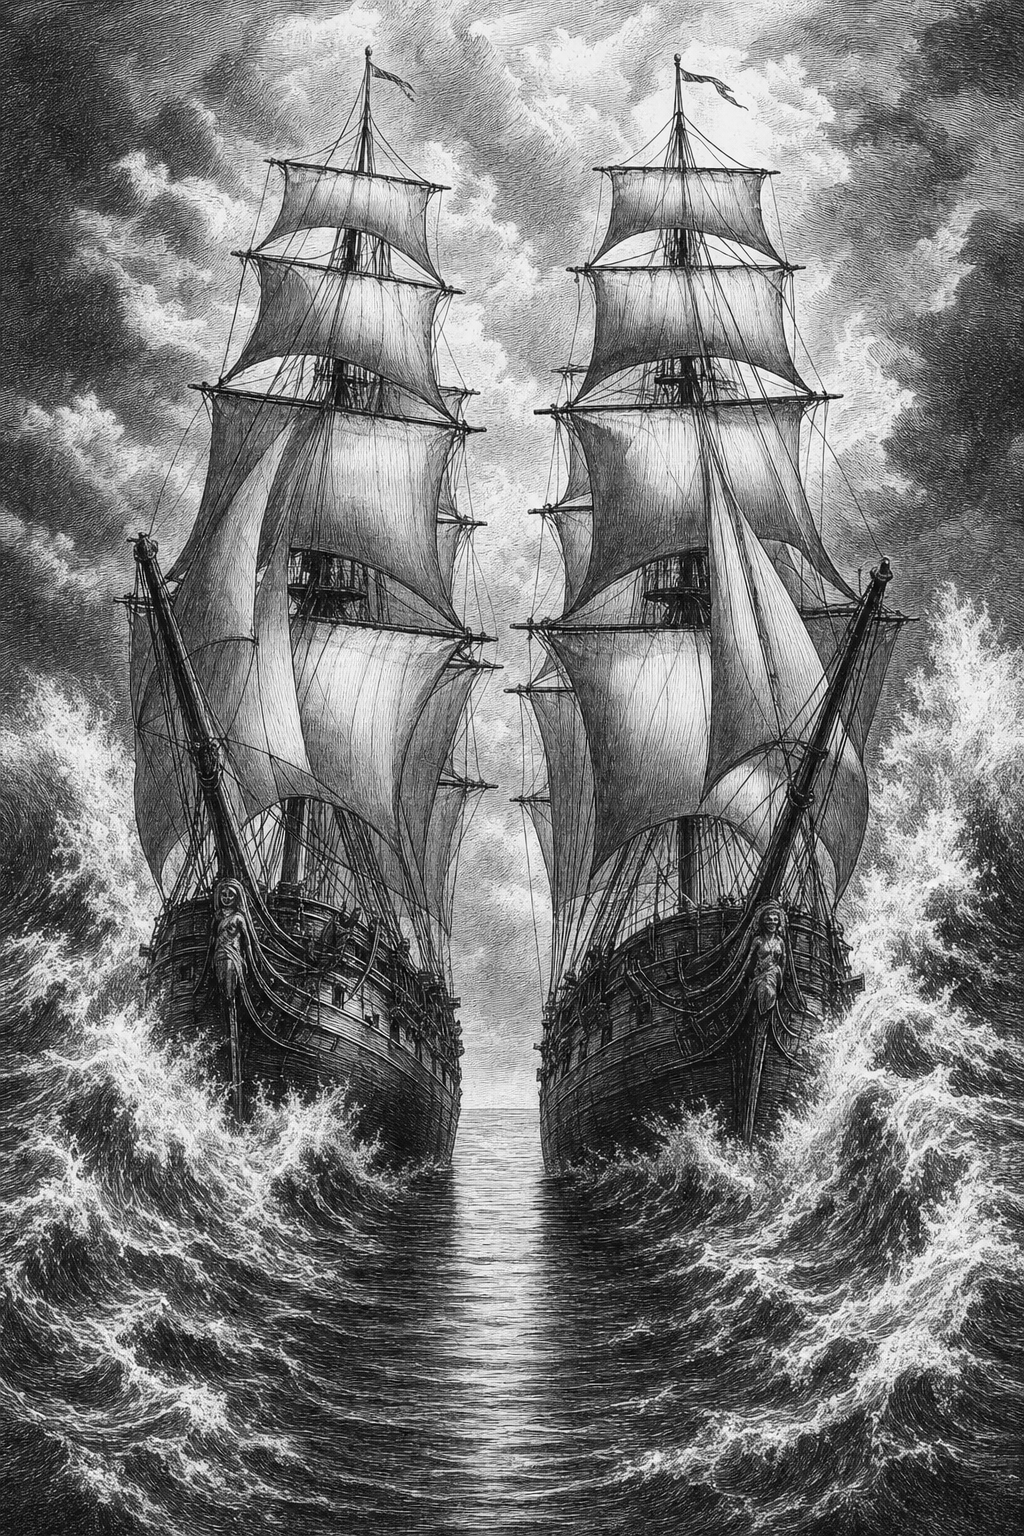
\includegraphics[height=0.92\textheight,width=\textwidth,keepaspectratio]{art/plate_two_ships}\end{figure}

The sketch even yields the right \emph{shape} of law, and this is worth pausing on. How much of your neighbor's shadow do you sit in? That depends on the angle it covers in your sky --- and the angular size of a shadow falls off as the square of the distance. Double the separation and the neighbor blocks a quarter of the directions it blocked before. An inverse-square law, not assumed, but \emph{inherited from geometry itself} --- from the mere fact that shadows shrink with distance in three-dimensional space. Newton's exponent, the sacred 2, stops being a decree and becomes a consequence: it is the dimensionality of the crowd, showing through. (And a reader of Tegmark's argument, quoted in this book's earliest notes, will see the same fact from the other side: in four spatial dimensions, shadow-geometry would give an inverse-cube law --- under which no orbit is stable~\cite{ehrenfest1917}. A universe of shadow-gravity that contains observers watching stable orbits will be a universe of three-dimensional crowds. The sketch does not just permit our dimensionality; it is most at home in it.)


\begin{figure}[htbp]
\centering
\begin{tikzpicture}[>=stealth]
  % ---- panel: distance d ----
  \begin{scope}
    \shade[ball color=black!70] (0,0) circle (0.30);
    \draw[black!30, dashed] (0,0) circle (2.05);              % the sky
    \shade[ball color=black!45] (3.0,0) circle (0.52);        % neighbour at d
    % shadow cone: tangents from observer centre to neighbour edges
    \fill[bbuGold!22] (0,0) -- (2.955,0.512) arc[start angle=9.85, end angle=-9.85, radius=3.0] -- cycle;
    \draw[black!45] (0,0) -- (2.955,0.512);
    \draw[black!45] (0,0) -- (2.955,-0.512);
    % covered arc of the sky, emphasised
    \draw[bbuRed, line width=1.8pt] (2.05,0) ++(9.85:0) arc[start angle=9.85, end angle=-9.85, radius=2.05];
    \node[anchor=north, align=center] at (1.4,-2.3) {\small at distance $d$: the neighbour\\ blocks this arc of the sky};
  \end{scope}
  % ---- panel: distance 2d ----
  \begin{scope}[yshift=-6.1cm]
    \shade[ball color=black!70] (0,0) circle (0.30);
    \draw[black!30, dashed] (0,0) circle (2.05);
    \shade[ball color=black!45] (6.0,0) circle (0.52);        % neighbour at 2d
    \fill[bbuGold!22] (0,0) -- (5.978,0.518) arc[start angle=4.95, end angle=-4.95, radius=6.0] -- cycle;
    \draw[black!45] (0,0) -- (5.978,0.518);
    \draw[black!45] (0,0) -- (5.978,-0.518);
    \draw[bbuRed, line width=1.8pt] (2.05,0) ++(4.95:0) arc[start angle=4.95, end angle=-4.95, radius=2.05];
    \node[anchor=north, align=center] at (2.6,-2.3) {\small at distance $2d$: half the angular width ---\\ one quarter of the sky directions};
  \end{scope}
\end{tikzpicture}
\caption{Newton's exponent, inherited from geometry. How hard the shadow push acts on a body depends on how much of its sky the neighbour blocks. Double the separation and the neighbour's angular width halves, so the blocked patch of sky --- an area on the sphere of directions --- shrinks to one quarter. The imbalance in the rain, and with it the push, falls off as the square of the distance: not a decree, but the dimensionality of the crowd showing through. (In four spatial dimensions the same geometry would give an inverse cube, under which no orbit is stable.)}
\label{fig:inversesquare}
\end{figure}

\section{Charge: Orbits and Orientation}

Gravity, in this sketch, is about \emph{blocking}. Charge is about \emph{circulation}.

Let some particles be orbited by others --- a central mote with companions wheeling around it in a plane, the whole assembly emitting and receiving smaller particles of its own. Now two such assemblies can differ in two purely geometric ways: the \emph{orientation} of the orbital plane, and the \emph{sense} of the circulation --- clockwise or counterclockwise, seen from a given side.

The old notes propose: this geometry \emph{is} charge. A ``positive'' object is such an assembly circulating one way; a ``negative'' object is the mirror arrangement. And the interactions follow from collisions of circulation, not from any charge-stuff:

Two assemblies circulating the \emph{same} way, meeting, superpose --- their streams run parallel where they meet, pile up, and press the assemblies apart. Like repels like, not by decree, but the way two water-vortices spinning the same sense shoulder each other away.

Two assemblies circulating \emph{opposite} ways interlock --- their streams at the meeting face run counter to each other, cancel, quiet the space between them. Each now shelters the other from the general agitation, and the shadow-push does the rest: unlike charges attract by the same mechanism as gravity, only fiercer, because circulation-cancellation quiets the space far more thoroughly than mere blocking thins it.

And orientation gives a third possibility that plain gravity lacks: two orbital planes at right angles to each other simply \emph{miss}. Their circulations neither pile nor cancel; they thread through one another's business without transacting, the way two polarizing filters\footnote{A polarizing filter passes only light whose sideways vibration lies along one axis; cross two at right angles and nothing gets through --- sunglasses and camera filters do it daily. (Dictionary: polarization.)} at ninety degrees pass no common light. In this sketch, that is what it is for two things to not interact: not a permission withheld, but a geometry that never meets.


\begin{figure}[htbp]
\centering
\begin{tikzpicture}[>=stealth]
  % ---------- (i) same sense: clash, repel ----------
  \begin{scope}[xshift=-3.85cm]
    \draw[black!60, ->, line width=0.9pt] (-0.85,0) ++(40:0.45) arc[start angle=40, end angle=340, radius=0.45];
    \draw[black!60, ->, line width=0.9pt] (0.85,0) ++(40:0.45) arc[start angle=40, end angle=340, radius=0.45];
    \fill[black!70] (-0.85,0) circle (0.10);
    \fill[black!70] (0.85,0) circle (0.10);
    % facing streams clash head-on (tip to tip)
    \draw[->, thick] (-0.14,0.42) -- (-0.14,0.10);
    \draw[->, thick] (0.14,-0.42) -- (0.14,-0.10);
    \node at (0,0) {\footnotesize$\times$};
    % repulsion
    \draw[->, bbuRed, line width=1.5pt] (-1.45,0) -- (-1.95,0);
    \draw[->, bbuRed, line width=1.5pt] (1.45,0) -- (1.95,0);
    \node[anchor=north, align=center, text width=3.2cm] at (0,-1.15)
      {\small (i) same sense:\\ streams meet head-on\\ --- pile up, repel};
  \end{scope}
  % ---------- (ii) opposite sense: align, attract ----------
  \begin{scope}[xshift=0cm]
    \draw[black!60, ->, line width=0.9pt] (-0.85,0) ++(40:0.45) arc[start angle=40, end angle=340, radius=0.45];
    \draw[black!60, <-, line width=0.9pt] (0.85,0) ++(20:0.45) arc[start angle=20, end angle=320, radius=0.45];
    \fill[black!70] (-0.85,0) circle (0.10);
    \fill[black!70] (0.85,0) circle (0.10);
    % facing streams run together: quiet corridor
    \fill[bbuBlue!14] (-0.30,-0.42) rectangle (0.30,0.42);
    \draw[->, black!45] (-0.14,0.38) -- (-0.14,-0.38);
    \draw[->, black!45] (0.14,0.38) -- (0.14,-0.38);
    % attraction
    \draw[->, bbuBlue, line width=1.5pt] (-1.65,0) -- (-1.25,0);
    \draw[->, bbuBlue, line width=1.5pt] (1.65,0) -- (1.25,0);
    \node[anchor=north, align=center, text width=3.2cm] at (0,-1.15)
      {\small (ii) opposite sense:\\ streams align and cancel\\ --- quiet space, attract};
  \end{scope}
  % ---------- (iii) orthogonal planes: no transaction ----------
  \begin{scope}[xshift=3.85cm]
    % left assembly: orbit seen face-on
    \draw[black!60, ->, line width=0.9pt] (-0.85,0) ++(40:0.45) arc[start angle=40, end angle=340, radius=0.45];
    \fill[black!70] (-0.85,0) circle (0.10);
    % right assembly: orbit seen edge-on (perpendicular plane)
    \draw[black!60, line width=0.9pt] (0.85,-0.45) -- (0.85,0.45);
    \draw[black!60, ->, line width=0.9pt] (0.85,0.45) -- (0.80,0.30);
    \draw[black!60, ->, line width=0.9pt] (0.85,-0.45) -- (0.90,-0.30);
    \fill[black!70] (0.85,0) circle (0.10);
    \node[black!55] at (0,0) {\small$\perp$};
    \node[anchor=north, align=center, text width=3.2cm] at (0,-1.15)
      {\small (iii) orthogonal planes:\\ the circulations thread past\\ --- no interaction};
  \end{scope}
\end{tikzpicture}
\caption{Charge as circulation. Each charged assembly sheds circulating streams of its own substance. (i)~Two assemblies circulating the \emph{same} sense present head-on streams where they face each other: the streams pile up and the assemblies are pressed apart --- like repels like. (ii)~\emph{Opposite} senses present aligned streams: they cancel, quiet the space between (shaded), and the shadow push does the rest --- opposites attract, by the same mechanism as gravity but fiercer. (iii)~Orbital planes at right angles neither pile nor cancel: the circulations pass through one another's business without transacting, as two crossed polarizing filters pass no common light.}
\label{fig:circulation}
\end{figure}

Push the same move one layer down and even the strange three-fingered rules of electromagnetism --- force at right angles to both motion and field, the rule every physics student memorizes with a contorted hand --- stop looking arbitrary. Where circulations meet circulations, the resultant push is perpendicular to both by the plain geometry of colliding streams. I do not claim the sketch derives Maxwell's equations; it does not, and Chapter 7 will be blunt about the gap. I claim the \emph{kind} of thing electromagnetism is --- directional, chiral, orthogonality-respecting --- is the kind of thing circulating crowds naturally produce, and that this is more than coincidence deserves.

Annihilation, too, falls out rather than being added. Two assemblies of opposite circulation that do not merely meet but \emph{collide} --- center into center --- have their orbits run head-on into each other's orbits. Counter-circulating streams at full interpenetration do not shelter; they cancel \emph{catastrophically}, each unwinding the other's circulation entirely. What remains is no longer two charged assemblies but their contents, flying loose: the crowd's raw particles, released. A positive and a negative object, meeting exactly, cease to be objects --- which is, in one line, what matter and antimatter have been observed to do since 1932.\footnote{1932: Carl Anderson's discovery of the positron, the electron's opposite twin; the mutual destruction of matter and antimatter followed into the textbooks.}

\section{States of the Crowd: Frozen and Gas}

A crowd of orbiting assemblies has collective conditions, the way water does. Call a region \emph{gas} when its assemblies wander freely, all agitation and passage. Call it \emph{frozen} when the circulations of neighboring assemblies have locked --- opposite-sense neighbors interlocked in the quiet-space embrace described above --- into a structure that holds its shape.

Two consequences from the old notes, both of which I still find striking:

First: \textbf{two frozen objects in a gas drift together.} Between them, each blocks and calms part of the other's agitation; the pressure of the gas between them is lower than the pressure outside; the outside wins. This is the shadow-push again, appearing at a new scale, unbidden --- the sketch's mechanisms repeat across levels without being re-installed, which is exactly what a layered universe ought to do. And two frozen objects pressed by a surrounding gas, if they are also moving, do not merely collide: they can fall into orbit around one another, captured by the very imbalance that draws them.

Second: \textbf{a frozen thing can melt.} A structure held by interlocked circulations holds only up to a certain agitation. Heat the crowd enough --- agitate the assemblies past what the interlocking can absorb --- and the structure lets go. The old notes put it in one sentence I have never improved on: \emph{a proton is perhaps frozen, and decays --- melts --- when it becomes hot enough.} Stability is not a permission granted to certain particles and denied to others; it is a phase, like ice. Matter persists because its region of the crowd is cold; push any matter into a hot enough region and it returns to gas. That the early universe --- hot beyond all measure --- should have been a place where no structure could freeze, and that matter as we know it should have condensed out as things cooled: in this sketch, that is not a special story requiring its own physics. It is what happens to any pond in autumn.


\begin{figure}[htbp]
\centering
\begin{tikzpicture}[>=stealth]
  % ------- (i) gas -------
  \begin{scope}[xshift=0.1cm]
    \foreach \p/\s in {(0.5,2.6)/1,(1.7,2.9)/-1,(2.6,2.3)/1,(0.9,1.7)/-1,(2.1,1.5)/1,(0.45,0.7)/1,(1.5,0.5)/-1,(2.7,0.8)/-1} {
      \draw[black!60, ->] \p ++(30:0.24) arc[start angle=30, end angle=300, radius=0.24];
    }
    \node[anchor=north, align=center, text width=3.0cm] at (1.6,-0.15)
      {\small (i) gas: assemblies\\ wander freely};
  \end{scope}
  % ------- (ii) frozen -------
  \begin{scope}[xshift=4.05cm]
    \foreach \i in {0,1,2} \foreach \j in {0,1,2} {
      \pgfmathparse{mod(\i+\j,2)==0 ? 1 : 0}
      \ifnum\pgfmathresult>0
        \draw[black!60, ->] ({0.55+\i*1.05},{0.55+\j*1.05}) ++(30:0.26) arc[start angle=30, end angle=310, radius=0.26];
      \else
        \draw[black!60, <-] ({0.55+\i*1.05},{0.55+\j*1.05}) ++(30:0.26) arc[start angle=30, end angle=310, radius=0.26];
      \fi
    }
    % bonds
    \foreach \i in {0,1} \foreach \j in {0,1,2} {
      \draw[black!25] ({0.55+\i*1.05+0.28},{0.55+\j*1.05}) -- ({0.55+\i*1.05+0.77},{0.55+\j*1.05});
      \draw[black!25] ({0.55+\j*1.05},{0.55+\i*1.05+0.28}) -- ({0.55+\j*1.05},{0.55+\i*1.05+0.77});
    }
    \node[anchor=north, align=center, text width=3.0cm] at (1.6,-0.15)
      {\small (ii) frozen: opposite senses\\ interlock into structure};
  \end{scope}
  % ------- (iii) two frozen bodies in gas -------
  \begin{scope}[xshift=8.0cm]
    % gas dots, denser outside than between
    \foreach \p in {(0.25,2.9),(0.9,3.1),(1.9,3.05),(2.7,2.85),(3.1,2.2),(0.2,2.1),(0.35,1.2),(0.2,0.4),(0.9,0.25),(1.8,0.2),(2.6,0.35),(3.15,0.9),(3.05,1.6),(1.35,2.75),(2.35,0.6)}
      \fill[black!50] \p circle (0.06);
    \fill[bbuGold!25] (1.25,1.05) rectangle (2.15,1.95); % quiet corridor between
    \draw[fill=black!35] (0.55,1.15) rectangle (1.25,1.85);
    \draw[fill=black!35] (2.15,1.15) rectangle (2.85,1.85);
    \draw[->, bbuBlue, line width=1.3pt] (0.35,1.5) -- (0.6,1.5);
    \draw[->, bbuBlue, line width=1.3pt] (3.05,1.5) -- (2.8,1.5);
    \node[anchor=north, align=center, text width=3.0cm] at (1.7,-0.15)
      {\small (iii) two frozen bodies\\ in a gas drift together};
  \end{scope}
\end{tikzpicture}
\caption{States of the crowd. (i)~Gas: assemblies wander, all agitation and passage. (ii)~Frozen: neighbouring circulations of opposite sense interlock into a structure that holds its shape --- matter as local winter; heat the crowd past what the interlocking can absorb and the structure lets go, which is what decay is. (iii)~Two frozen bodies in a gas shelter each other: the agitation between them (shaded) is calmer than the agitation outside, and the outside wins --- the shadow push reappearing at a new scale, unbidden.}
\label{fig:frozengas}
\end{figure}

Even the charged objects themselves, the notes suggest, are frozen things --- but imperfectly frozen: they \emph{sublimate}, shedding small circulating pieces of themselves in all directions, the way ice smokes in dry winter air. That shed circulation is the ``field'' around a charge --- not a field at all, but weather: the object's own substance, departing, carrying its circulation-sense outward to interlock or collide with whatever it meets.

\section{Light}

What, then, is light? The old notes give one line: \emph{light is an object orbited by another, in motion --- a wave.} I will unfold it first exactly as written --- and then, because writing this book taught me where it fails, rebuild it into something stronger out of this chapter's own parts.

Take the smallest assembly there is at a given layer --- one mote and one companion, wheeling. Set the pair moving through the crowd. What passes any fixed point is a \emph{circulation arriving periodically}: the companion swings near, swings far, near, far, as the pair travels --- a regular beat of push delivered to everything along the path. A traveling circulation is a traveling oscillation. It has a frequency: the wheeling rate. It has an orientation: the plane of the orbit --- and there is polarization, not as an extra property bolted on, but as the geometry the object could not help having. Turn two such travelers' planes perpendicular and they transact nothing with each other, and interact differently with everything else --- the polarizing filter again, now as optics.

And the oldest of all the questions about light --- is it a particle or a wave? --- receives, in the sketch, the mildest possible answer: it is a particle \emph{doing} a wave. The traveling pair is as localized as any particle, and delivers its pushes in discrete arrivals; the pattern of those arrivals along the path is as periodic as any wave. The sketch does not pretend this settles a century of quantum mechanics. But it is worth noticing that the toy's most economical object --- two motes and a motion --- arrives already wearing both costumes.


\begin{figure}[htbp]
\centering
\begin{tikzpicture}[>=stealth]
  % ------- main: the pair in motion, companion tracing a wave -------
  \draw[black!35, dashed] (0,0.9) -- (7.5,0.9);
  % companion's trace
  \draw[bbuGold, line width=1.0pt, domain=0:6.6, smooth, samples=80]
    plot (\x,{0.9+0.62*sin(\x*120)});
  % past positions of the mote (fading)
  \fill[black!20] (0.75,0.9) circle (0.09);
  \fill[black!35] (2.9,0.9) circle (0.09);
  \fill[black!50] (5.05,0.9) circle (0.09);
  % current pair
  \fill[black!75] (6.6,0.9) circle (0.11);
  \draw[black!55] (6.6,0.9) ellipse [x radius=0.42, y radius=0.62];
  \draw[black!55, ->] (6.6,0.9) ++(60:0.5) arc[start angle=60, end angle=140, x radius=0.42, y radius=0.62];
  \fill[black!70] ({6.6+0.42*cos(20)},{0.9+0.62*sin(20)}) circle (0.07);
  \draw[->, line width=1.1pt] (6.85,1.95) -- (7.55,1.95);
  \node[anchor=south] at (7.2,2.0) {\small motion};
  \node[anchor=north, align=center, text width=6.6cm] at (3.6,-0.25)
    {\small the smallest assembly --- one mote, one wheeling companion --- set moving: what passes any fixed point is a circulation arriving periodically};
  % ------- inset: perpendicular plane = the other polarization -------
  \draw[black!35] (8.6,0.0) -- (10.5,0.0);
  \draw[black!60, line width=0.9pt] (9.55,0.28) -- (9.55,1.52);
  \draw[black!60, ->, line width=0.9pt] (9.55,1.52) -- (9.48,1.30);
  \draw[black!60, ->, line width=0.9pt] (9.55,0.28) -- (9.62,0.50);
  \fill[black!75] (9.55,0.9) circle (0.11);
  \node[anchor=north, align=center, text width=2.5cm] at (9.55,-0.25)
    {\small the same traveler,\\ plane turned $90^{\circ}$:\\ polarization};
\end{tikzpicture}
\caption{The first sketch of light: an object orbited by another, in motion --- a particle doing a wave. The traveling pair is as localized as any particle and delivers its pushes in discrete arrivals; the pattern of those arrivals along the path is as periodic as any wave, with a frequency (the wheeling rate) and an orientation (the plane of the orbit). Turn the plane ninety degrees (right) and you have the other polarization --- not a property bolted on, but geometry the object could not help having. The section keeps this picture --- demoted: as the portrait of a localized wave-packet of the medium, not the traveler itself.}
\label{fig:lightpair}
\end{figure}

That was the sketch as my notes first drew it, and I have kept it because it earns its keep --- but writing this book has taught me its two failures, and they are not small ones. First: \emph{universal} $c$. Every pair, whatever its wheeling rate, whatever its history, moves at exactly the same speed --- the same to one part in a thousand million million, dispersionless across a billion years of travel. Nothing about a composite assembly explains that; assemblies should vary. Second: interference. A lone traveling pair does not bend around corners, and it cannot cancel itself into the dark bands of the two-slit pattern; those are things \emph{waves in a medium} do, and no solitary traveler does them. Light's two most famous behaviours, and the pair can do neither.

But this chapter has already built, for other reasons, exactly the thing that can. The First Rule made the vacuum a crowd. The frozen state made a crowd that holds its shape --- interlocked circulations, a structure with tension in it. And a structured medium with tension \emph{sings}: it carries transverse waves of its own substance, at a speed set not by the wave's history but by the medium --- one crowd, one wave speed, for every frequency, from every source, the way sound in air does not care who shouted. So here is the upgrade, and I state it as a replacement of mechanism, not of image: \emph{light is not a traveler through the vacuum-crowd; light is the vacuum-crowd's own song.} A transverse wave \emph{of} the medium. At one stroke the two failures dissolve: universal $c$ is a medium property, dispersionlessness is the medium's linearity, and interference, diffraction, the dark bands --- these are what medium-waves do natively, no purchase required. Refraction arrives free: light slows in glass because glass is a denser, mixed crowd. The wave was never the hard part. The hard part was always the lump.

And the lump is bought with the coin this book already owns: the gap. A \emph{quantized} medium's waves come in lumps --- condensed-matter physics has a name for exactly this, the phonon,\footnote{The phonon: the quantum of sound in a crystal --- vibration of a lattice, which quantum mechanics obliges to come in discrete lumps. Proof by existence that a medium's waves can be particles. (Dictionary.)} the particle of a crystal's sound --- and the photon, in this picture, is the vacuum-crowd's transverse phonon: the smallest lump of the medium's song that the gap permits. The traveling pair of the figure is not discarded; it is demoted and preserved. It is the \emph{portrait} of a wave-packet --- what a localized lump of the medium's wave looks like when you squint: compact, periodic, arriving in discrete pushes, carrying its plane. The sketch had the right picture and the wrong ontology: wave-first, with the particle emergent, is the right way round --- and it is, for what it is worth, the way the twentieth century's own field theory rounds it too.

\begin{figure}[htbp]
\centering
\begin{tikzpicture}[>=stealth]
  % ---- (a) gravity: the crowd's push (streaming rain, shadow) ----
  \begin{scope}[xshift=-2.95cm]
    \foreach \p/\a in {(-1.9,1.55)/-40,(-1.2,1.8)/-75,(-0.3,1.7)/-100,(0.6,1.85)/-120,(1.5,1.6)/-140,(-2.0,0.0)/-15,(1.95,0.25)/195,(-1.85,-1.35)/35,(-0.9,-1.7)/70,(0.1,-1.8)/95,(1.1,-1.65)/115,(1.9,-1.3)/150}
      \draw[->, black!45] \p -- +(\a:0.55);
    \fill[bbuGold!25] (-0.62,-0.17) rectangle (0.62,0.17);
    \shade[ball color=black!65] (-0.85,0) circle (0.26);
    \shade[ball color=black!65] (0.85,0) circle (0.26);
    \draw[->, bbuBlue, line width=1.2pt] (-1.5,0) -- (-1.18,0);
    \draw[->, bbuBlue, line width=1.2pt] (1.5,0) -- (1.18,0);
    \node[anchor=north, align=center, text width=4.5cm] at (0,-2.1)
      {\small (a) gravity: the crowd's \emph{push} ---\\ streaming rain, and its imbalance};
  \end{scope}
  % ---- (b) light: the crowd's song (frozen lattice, transverse packet) ----
  \begin{scope}[xshift=2.95cm]
    % lattice rows with a transverse wave-packet
    \foreach \r in {-0.55,0,0.55} {
      \foreach \i in {0,...,16} {
        \pgfmathsetmacro{\x}{-2.0+\i*0.25}
        \pgfmathsetmacro{\env}{exp(-((\x)*(\x))/0.9)}
        \pgfmathsetmacro{\dy}{0.42*\env*sin(\i*80)}
        \fill[black!60] (\x,{\r+\dy}) circle (0.045);
      }
    }
    % envelope hint
    \draw[bbuGold, dashed, domain=-2.0:2.0, smooth, samples=50]
      plot (\x,{0.55+0.42*exp(-\x*\x/0.9)});
    \draw[bbuGold, dashed, domain=-2.0:2.0, smooth, samples=50]
      plot (\x,{-0.55-0.42*exp(-\x*\x/0.9)});
    \draw[->, line width=1.0pt] (1.15,1.35) -- (1.85,1.35);
    \node[anchor=south] at (1.5,1.4) {\small travels};
    \node[anchor=north, align=center, text width=4.5cm] at (0,-2.1)
      {\small (b) light: the crowd's \emph{song} ---\\ the frozen lattice itself waving; the lump is the photon};
  \end{scope}
\end{tikzpicture}
\caption{The rain and the song --- the same crowd, doing its two things. (a)~Gravity is what the crowd's \emph{streaming} does: an omnidirectional rain, and bodies pushed by nothing but its imbalance --- the shadow mechanism of this chapter's opening. (b)~Light is what the crowd's \emph{structure} does: the frozen, circulation-strung lattice waving transversely across the line of travel, the disturbance confined to a lump (dashed envelope) --- a wave-packet, the photon. One medium; a push and a song; and the difference between the two is the difference between weather and music.}
\label{fig:rainandsong}
\end{figure}

Charge then closes a loop I did not plan. Charge, in this chapter, is circulation; and a circulation \emph{shaken} --- an assembly accelerated --- cannot help disturbing the lattice it is embedded in: it sheds medium-waves. That is precisely what electromagnetism reports --- accelerated charges radiate --- now with a mechanism under it. And absorption runs the film backward: a resonant circulation catches a passing wave whole, or not at all, because the gap forbids partial purchase --- and there, in one sentence, is the photoelectric effect that began the quantum century~\cite{einstein1905photo}. One more consequence, and it is the one this book was always going to reach: our light is a wave of \emph{our} vacuum --- the crowd one layer down. But that crowd's own inhabitants have their own vacuum, the crowd below \emph{them}, with its own tension and its own transverse song --- faster than ours, if the layers quicken downward. \emph{Every layer has its own light, and its own} $c$. The speed of light is the loudest constant of our layer, not of the world: locally special, not globally special, now said of $c$ itself. What that buys, and what it costs, is Chapter~7's business.

\section{Why Things Are Alike}

One question remains that any mechanical universe must answer, because it is the question mechanics is worst at: why are things \emph{identical}? Every electron matches every other, everywhere, exactly. A universe of crowds and collisions ought, one would think, to produce endless slop --- assemblies of every size, orbits of every radius, a smear of almost-electrons. It produces instead a crisp catalogue of a few exact species. Why?

The old notes offer two answers --- one answer, I have come to think, seen from two sides --- and the writing of this book has forced a third.

The first: identical things are identical because they are \emph{made the same way} --- shed, as the sublimation picture has it, by parents that are themselves identical, the way every snowflake's sixfold symmetry is inherited from the one geometry of the water molecule. Identity propagates: like begets like, and the catalogue is a genealogy.

The second: the crowd itself may permit only certain assemblies to persist. Circulations interlock stably only at particular relations of size, speed, and spacing --- the way a plucked string, whatever you do to it, sounds only its own discrete harmonics, because only whole numbers of half-waves fit between its ends. Every other vibration dies at once; the survivors are exact, and exactly repeatable, not because anyone tuned them but because \emph{fitting} is an all-or-nothing affair. On this view the electron is not a thing that happens to be common; it is a \emph{resonance of the crowd} --- one of the few closed circulations that does not immediately unwind --- and it is identical everywhere for the same reason the third harmonic of every equal string is identical: the arithmetic of fitting has no almost.

And the third answer runs \emph{upward} through the layers, and it is a selection. Take the sketch's basic object --- a mote with a companion wheeling around it --- and ask what it needs in order to \emph{last}: to hold its orbit long enough for anything to be built from it. It needs the rain from below to be steady. Uniform in time, and uniform across the great distances the assembly will roam --- because a patchy crowd below means a varying push, and a varying push means orbits that drift, structures that shake themselves apart, nothing that accumulates. So long-lived structure at any layer \emph{certifies} the sameness of the layer beneath it, over exactly the reach and the ages that the structure has survived. Turn the certificate around and it becomes an explanation: things are alike down there wherever things persist up here --- not because unlikeness is impossible, but because unlikeness is \emph{uninhabitable}. Regions sitting over a motley crowd host no lasting assemblies, no chemistry, no memory, no one to ask why things are alike. We find identical electrons for the same kind of reason we find ourselves on a planet with water: the places without are not places where finding happens. My earliest notes contained this in embryo without my seeing it --- ``an expansion factor that limits the possibilities; otherwise, it disappears.'' \emph{Otherwise it disappears} is a selection principle. This is its grown form.

The three answers are not rivals; they stack, each carrying the part the others cannot. Selection explains the \emph{demand} --- a substrate must be uniform or bear nothing --- but selection's tolerance is loose: orbits forgive perturbations of a percent, while electrons match to twelve decimals, an overshoot no stability requirement could ever impose. The overshoot is resonance's part: the only way a crowd \emph{can} be uniform is by being exact, because populations of almost-alike assemblies unravel into the sharp harmonics or into nothing. Uniform-or-nothing; and uniform-means-exact; and then genealogy propagates the exactness onward, like begetting like. One honest horizon comes with the selection answer, and I state it rather than hide it: it predicts uniformity precisely and only \emph{where there is structure to check it}. Variation, if the tower contains any, lives where nothing survives to record it --- so when our instruments report the constants of physics steady across billions of light-years of quasar light~\cite{uzan2003,damourdyson1996}\footnote{A quasar is the violently bright core of a distant galaxy; its light, crossing most of the visible universe, is stamped on the way with the fingerprints of atoms it passes through --- so it carries a record of whether the constants of physics were the same out there, back then. (Dictionary.)}, they confirm exactly what the filter guarantees they would, and can never catch the exception. Looking is itself a certificate.

I flag, honestly, what the reader may already suspect: the resonance answer is quantization --- the discreteness of nature --- appearing \emph{inside} the sketch as a consequence of continuous mechanics, rather than as a rival to it. Whether that appearance is genuine or a conjuring trick is perhaps the most important open question in this book, and Chapter 7 will press on it with both hands. If discreteness can emerge from crowds, the sketch's deepest problem dissolves. If it cannot, the sketch has a wound that does not close --- though I will say now what I could not have said when I first wrote this sentence: the pressing, in Chapter~7, went better than I feared. It found doors as often as walls.

\section{The Sketch, Standing}

That is the toy, wound up and running. One flux, and shadows in it: gravity, with its inverse square inherited from geometry. Circulation, and its collisions: charge, likeness repelling, opposites embracing, right angles ignoring one another, head-on meetings annihilating. Phases of the crowd: matter as local winter, decay as thaw, the early universe as a heat in which nothing could freeze. A traveling circulation: light, wearing particle and wave at once, polarized by its own geometry. And a catalogue of identical things, as harmonics of what can persist.

Underneath it all, the first rule, holding everything: there is no emptiness anywhere in this universe. Every layer's void is the layer below, crowded and busy; every ``force through space'' is that crowd, pushing; and that crowd's own space is another crowd, without end. Nothing pulls. Nothing is fundamental. Nothing is magic.

It is only a sketch, and I have kept my promises about honesty everywhere else in this book; I will keep them here. The next chapter is a list of the places where this beautiful toy, tested against the world, breaks. I wrote both chapters, and I find I love the toy no less for what the tests do to it. A sketch that can be broken in \emph{specific places} is a sketch that says specific things --- and that, not survival, was the standard a toy universe had to meet.

\En

\begin{draftnote}
Craft notes: (1) The inverse-square-from-shadow-geometry derivation is the chapter's strongest physics moment --- verify the solid-angle argument carefully; it is correct for absorption-shadowing at separations large compared to the bodies, which should be stated or footnoted. (2) The string-harmonics answer to identicalness is doing enormous work --- it is, in effect, a claim that quantization could be emergent; Ch. 7 must treat it as a claim, not a fact. (3) The Maxwell disclaimer and the QM disclaimer are load-bearing for credibility --- do not soften them in revision. (4) Consider a simple figure: two bodies, the flux, the mutual shadows. One drawing may spare three paragraphs. (5) Constancy-of-constants: sources now in ref.bib (uzan2003 = Rev.~Mod.~Phys.~75, 403; damourdyson1996 = the Oklo bound, $\Delta\alpha/\alpha < 10^{-7}$ over $\sim$2 Gyr $\approx$ 0.1 ppm). Author to read the passage's two sentences once against Uzan's abstract --- the book's ``parts per million'' is the constraint side and looks safe. (6) [resolved: ships lore hedged in prose per PROSE\_PATCHES\_stage1.md; physics retained.]
\end{draftnote}

\chapter{\emph{Where It Breaks, and What That Teaches}}
\chapterart{ch7_cracked_orrery}
\draftstatus{Draft 1}

\lettrine{I}{} promised, at the start of the last chapter, to attack the toy myself. This chapter keeps the promise, and I want to state the rules of the attack as plainly as I stated the rules of the sketch.

The attacks below are not quibbles and they are not strawmen. They are the strongest objections I know --- most of them are the \emph{historical} objections, the ones that actually killed the mechanical program in the hands of people who wanted it to succeed. I will present each at full force, then give the best reply the toy can make, and then say honestly whether the reply closes the wound or only bandages it. The reader should keep score. By my own count the toy leaves this chapter alive and changed. Five wounds: one three hundred years old, answered at last only in the tower's own strange currency; one that turned, on inspection, into a specification with a laboratory address; one still leaning against; one that grew three answers and a door; and a fifth --- the deepest --- where a theorem is aimed at this book's first sentence, and the book's earlier purchases turn out, on the word of the theorem's own author, to be the recommended remedy. The reader should keep score, and at the chapter's end I will keep it with you, in a single table.

That is not a preface of despair. A model that can be wounded in \emph{specific places} is a model that says specific things; the alternative --- a picture so vague nothing can hurt it --- was never worth having. Here are the places.

\section{First Wound: The Pincer of Drag and Heat}

The oldest objection is Newton's own, raised against Fatio --- the first shadow-gravity man --- before Le Sage was born, and it has never been answered. It goes like this.

The flux, in the sketch, is what pushes. But a planet is not sitting still in the flux; it is \emph{moving} through it --- the Earth at thirty kilometers every second around the Sun. A body moving through rain meets more rain on its front face than its back, exactly as a runner in a downpour is wetter on the chest than the shoulders. So the flux, whatever else it does, must \emph{resist motion}: every orbiting body feels a headwind. A headwind, sustained over orbits, is death --- the planet sheds momentum, spirals inward, and falls into its sun. The timescale can be argued about; the direction cannot. Shadow-gravity, taken neat, predicts that no solar system is stable. Ours has run for four and a half billion years.

The toy's reply is the classic one: make the flux \emph{fast}. The headwind a body feels scales with the ratio of its speed to the flux's speed; if the massions move enormously faster than any planet --- faster than light, in Le Sage's later rescues --- the drag shrinks toward nothing, and orbits survive.

And here the pincer closes, because the rescue feeds the second monster. The flux does not only push bodies; it must \emph{deposit energy} in them --- that is what being absorbed or scattered means; you cannot take momentum from a stream without taking some of its punch. Speed the flux up to save the orbits, and every absorption delivers more energy. The nineteenth century did this arithmetic --- Maxwell pressed the objection, and Poincaré finally ran the numbers to the end --- and the verdict was not a discrepancy but an absurdity: a flux energetic enough to produce the gravity we measure, moving fast enough to spare the orbits we see, would heat the Earth at a rate that would vaporize it --- not over ages, but promptly. \emph{(Exact figures to be checked against Poincaré's calculation before publication; the qualitative verdict is not in dispute.)}

That is the pincer, and I want the reader to feel its shape, because it is the shape of a serious refutation: the two objections cannot be answered \emph{together}. Slow flux: orbits decay. Fast flux: planets glow. Poincar\'e, in 1908, put numbers to the jaws: to evade the drag, the corpuscles must move at no less than $24\times10^{17}$ times the speed of light; and at the absorption rate gravity requires, the Earth would heat by $10^{26}$ degrees per second --- an intake some $10^{20}$ times everything the sun emits. Those are not figures a model recovers from. Every knob the model has, turned to fix one wound, tears the other wider. Kelvin tried the cleverest escape --- let bodies re-emit the absorbed flux, passing the energy through rather than keeping it --- but re-emission, done isotropically,\footnote{Isotropic: the same in every direction. An isotropic rain pushes nothing anywhere; only its imbalances act. (Dictionary.)} also re-emits the \emph{momentum}, and the gravity disappears with the heat. The pincer has held for three hundred years, and within any single layer I have no new answer to it and will not pretend otherwise. But this book is not a single layer --- and whether the \emph{tower} has an answer is a question the pincer's three centuries never had occasion to face. This section will put one on the table, with its invoice attached, and the reader will judge the price.


There is an escape more tempting than Kelvin's, and I owe it a proper burial, because every thoughtful reader reaches for it --- I reached for it myself. Two things are conserved in any collision: momentum, $mv$, and energy; and in a perfectly \emph{elastic} collision the energy stays kinetic, $\tfrac{1}{2}mv^{2}$, none of it degraded to heat. So: let the massions bounce. Perfectly elastic collisions --- no absorption, no heating, and the second jaw of the pincer never closes. Conservation itself seems to offer the way out.

It does not --- but the reason deserves more than assertion, because the rubber-ball picture feels so obviously right: surely a bouncing body still \emph{blocks}; surely there is still a shadow. Here is where the picture misses. An elastic body does not only block the balls that were heading for you. It also \emph{redirects, into you, balls that were going to miss you} --- every ball that bounces off it leaves in a new direction, and some of those new directions point exactly your way. So the ledger has two entries: the blocked loss from behind the body, and the scattered gain off its surface. The whole question is whether the gain fills the loss, and for perfect elasticity the answer is exact: it fills it to the last ball.

The cleanest way to see it is the mirror in the glowing sky. An absorbing body in an isotropic rain is a \emph{black} ball against a uniformly bright sky: from where you stand there is a dark patch in its direction, and the imbalance of the rain pushes you toward the dark --- that is the shadow, and it is real. But a perfectly elastic body is a \emph{mirror} ball in that same sky, and a mirror ball in a uniformly glowing sky is invisible: from every viewing angle its surface shows a reflection of the sky, at exactly sky brightness. There is no dark patch; there is nothing to be pushed toward. Formally, in one line: a uniform isotropic flux is a \emph{stationary state} of elastic bouncing --- reflections preserve speeds and merely swap directions, so the rain is exactly as isotropic with the mirror present as without it, and an isotropic rain pushes nothing anywhere. A shadow, in the steady state, requires balls to be \emph{removed}, and elastic collisions remove none. (Two honest concessions to the intuition. Insert the bodies suddenly and there is a brief transient shadow while the scattered flux fills in; the steady state erases it. And the intuition was trained on honest rubber, which is never perfectly elastic --- every real bounce steals a little momentum, and casts exactly that much shadow.) The theory's nineteenth-century examiners knew all of this: Le Sage gravity does not merely tolerate inelastic collisions, it \emph{requires} them. No absorption, no gravity.


Push once more, because the objection has a sharper form and it deserves the same full-strength treatment. Take two plates, close together, in the elastic rain, and let the plates be imperfect mirrors: say one ball in ten passes through. Surely now there is a shadow pull --- the gap between the plates is hard to enter, so it should sit nearly empty, outside pressure unbalanced, plates pressed together. The intuition is quantitative and it feels irresistible. And it fails on a cancellation so clean it is worth watching happen. Balls enter the gap by transmission, at a rate proportional to $T$ times the outside flux, with $T$ the one-in-ten. But balls \emph{leave} the gap the same way: a ball trapped between the plates strikes a plate from the inside and has the same one-in-ten chance of getting out, nine-in-ten of being bounced back in. Steady state means in-rate equals out-rate --- $T$ times the outside flux equals $T$ times the inside flux --- \emph{and $T$ cancels.} The interior fills to exactly the ambient density whether the plates pass one ball in ten or one in ten thousand. A low transmission does not lower the level the gap fills to; it only slows the clock. Each ball that sneaks in bounces, on average, ten times before escaping, and that long imprisonment is precisely what stocks the gap to full pressure. The gap is hard to enter, and \emph{equally hard to leave} --- the two difficulties are the same difficulty, and they cancel. It is the physics of a box with a pinhole in ordinary air: the size of the hole sets how long the box takes to fill, and has no say at all in what it fills \emph{to}.

Two special cases survive, and honesty means naming both, because one of them is real physics with a name. First, seal the plates perfectly ($T=0$) around a gap that was \emph{prepared} empty: then yes --- outside pressure, no inside pressure, and the plates slam together. That is the Magdeburg hemispheres\footnote{1654, Otto von Guericke: two evacuated half-spheres of copper, pressed together by nothing but the weight of the air --- teams of horses could not pull them apart.}, and it is real; but the vacuum must be manufactured and sealed, any leak fills it, and no natural approach of two bodies produces it --- bringing plates together in the rain traps ambient balls between them rather than excluding them. Gravity cannot depend on every gap in the universe having been factory-evacuated. Second --- and this is the beautiful one --- make the gap \emph{smaller than one ball}. Now no ball fits between the plates at all, transmission be damned; the interior is empty not by kinetics but by geometry; the outer faces feel full pressure, the inner faces feel nothing, and the plates are genuinely pushed together, with perfectly elastic balls. This is not hypothetical. It is the \emph{depletion force} of colloid physics~\cite{asakuraoosawa1954}\footnote{Colloids: particles around a thousandth of a millimetre, suspended in a fluid --- milk and paint are colloids. Their physics is where the depletion force lives.} --- a measured, textbook attraction between particles suspended in a bath of smaller hard spheres --- and it is, precisely, elastic Le Sage shadowing. Nature runs the mechanism. But look at its range: the attraction exists only while the gap is smaller than one corpuscle diameter, because the moment a ball \emph{can} fit, the steady state floods the gap and the force dies. The elastic shadow is geometric, not kinetic, and geometric shadows do not reach. There, stated by nature herself, is the theorem against elastic gravity: the honest elastic version of the shadow push exists, is real, has a name --- and has a range of one massion. Gravity holds the Moon at four hundred thousand kilometres.

And that requirement exposes the pincer's deepest form, sharper than drag-against-heat: \emph{the gravity and the heating are the same event, read in two currencies.} The momentum a body absorbs from the stream is the force; the energy that rides in with that momentum is the heat; and for a fast corpuscle the two come bundled at a fixed exchange rate --- energy per unit of momentum equal to half the corpuscle's speed --- so the faster the flux (and the drag objection has already forced it to be enormously fast), the more energy every unit of gravitational push must deliver. Worse still: the push is the \emph{net} imbalance of the rain, the small difference between nearly equal bombardments, while the heating goes with the \emph{gross} absorption from all sides at once. The force is a residue; the heat is the whole meal. Conservation of $mv$ and conservation of $\tfrac{1}{2}mv^{2}$ are not the toy's way out. They are the pincer's two jaws, named.

What the toy \emph{can} say --- and it is worth saying, though it is a retreat and I mark it as one --- is that the pincer bites a specific implementation: absorption of a corpuscular flux at \emph{our} layer. Whether every mechanism a layered crowd can offer --- collective modes, circulation-transfers, the subtler commerce of Chapter 6's interlocked assemblies --- must fall to the same arithmetic is genuinely less clear; nobody has run Poincaré's numbers against a crowd that is itself made of crowds. But a hope that has not been calculated is a hope, not a defense --- unless the hope can be given a shape, and there is one shape the tower makes possible that was never available to Le Sage. It rests on one assumption this book finds natural: \emph{lower layers are faster} --- the characteristic speeds of each layer's crowd exceed those of the layer above.

Recall the exchange rate that closed the pincer: energy per unit of momentum equal to half the channel's speed. Read it again, as a market. Energy is momentum-\emph{expensive} in slow channels and momentum-\emph{cheap} in fast ones. So let a body buy its momentum in the slow market --- the layer's own flux, where the shadow lives and the push is delivered --- and \emph{sell its energy in the fast market}: dispose of the absorbed energy into sub-layer channels, where the same energy carries almost no momentum and cannot repaint the shadow. This is precisely what Kelvin's escape lacked. He re-emitted into the \emph{same} market, and full-speed isotropic re-emission is elastic scattering by another name --- the mirror ball, no gravity. Down-conversion into a faster layer evades him, because the disposal is momentum-cheap by the ratio of the two speeds. And the fourth wound of this chapter, waiting below, supplies the valve unbidden: matter whose our-layer modes are \emph{gapped} cannot thermalize the throughput here --- the energy is refused admission to our channels and forced downward, through every body, past every thermometer, into the basement. Several layers may contribute their own shadow components to the push; the energy of all of them drains the same way. The Earth never warms, because the Earth was never the destination.


\begin{figure}[htbp]
\centering
\begin{tikzpicture}[>=stealth]
  % layer bands
  \fill[black!5]  (0,3.2) rectangle (9.6,4.6);
  \fill[black!9]  (0,1.6) rectangle (9.6,3.0);
  \fill[black!13] (0,0.0) rectangle (9.6,1.4);
  \node[anchor=east] at (9.45,4.28) {\small layer $N$ --- flux speed $u$};
  \node[anchor=east] at (9.45,2.68) {\small layer $N{+}1$ --- faster: $w \gg u$};
  \node[anchor=east] at (9.45,1.08) {\small layer $N{+}2$ --- faster still};
  \node at (4.8,-0.32) {\small $\vdots$};
  % the body in layer N
  \shade[ball color=black!65] (2.6,3.9) circle (0.5);
  % slow flux: momentum bought
  \draw[->, bbuBlue, line width=1.3pt] (0.4,3.9) -- (1.98,3.9);
  \draw[->, bbuBlue, line width=1.3pt] (4.8,3.9) -- (3.22,3.9);
  \draw[->, bbuBlue!70] (0.7,4.25) -- (1.85,4.25);
  \draw[->, bbuBlue!70] (4.5,3.55) -- (3.35,3.55);
  \node[anchor=south, align=center, text width=5.4cm] at (2.6,4.72)
    {\small momentum bought in the slow market: the push};
  % the valve at the body's floor
  \draw[line width=1.2pt] (2.18,3.34) -- (2.45,3.34);
  \draw[line width=1.2pt] (2.75,3.34) -- (3.02,3.34);
  \node[anchor=east, align=center, text width=2.2cm] at (2.05,3.05)
    {\small the gap:\\ the valve};
  % energy sold down
  \foreach \x in {2.35,2.6,2.85} \draw[->, bbuRed] (\x,3.30) -- (\x,2.88);
  \foreach \x in {2.05,2.35,2.6,2.85,3.15} \draw[->, bbuRed!75] (\x,1.58) -- (\x,1.18);
  \node[anchor=west, align=center, text width=3.0cm] at (3.35,2.35)
    {\small energy sold down, into ever-faster channels --- momentum-cheap};
\end{tikzpicture}
\caption{The cascade escape, drawn. A body buys its momentum in its own layer's slow flux --- the shadow push, the gravity --- and sells the energy that rides in with it \emph{downward}, into the faster channels of the layers below, where the same energy carries almost no momentum and cannot repaint the shadow. The gap of the fourth wound is the valve: our layer's modes refuse the throughput, so it passes through matter without warming it. Each layer's books are covered by the layer above --- and the reader knows, by now, the price of a ledger with no first account.}
\label{fig:cascade}
\end{figure}

Now the price, because this book does not sell escapes without their invoices. Run the books layer by layer. Each layer's flux is being absorbed --- that is the gravity --- so it depletes unless resupplied; resupplied from the layer above, by the same mechanism; and that layer from the one above it, without end. \emph{Every layer's energy account is covered by the layer above, and there is no first account.} The reader has seen this structure before, at the centre of Chapter~3: it is induction with the base case deleted --- the tower's grounding problem, returned in the currency of joules. The cascade is the explanatory regress made physical: locally conserved at every layer, globally never closed, every book balanced by the next book, and the balancing never completing. The rescue of the pincer is available at exactly the price the whole book has already chosen to pay --- and whether that price buys a solution or a deferral is the same question as Chapter~3, on which I have already, publicly, taken my side. Two further costs ride along, flagged rather than fatal: the resupply must be steady enough that the strength of gravity has not drifted measurably over the ages~\cite{hofmann2018}, and the graininess of the absorption must be fine enough to hide from the quietest accelerometers ever built~\cite{armano2018}. Both are checkable, and neither has been checked.

So the honest scoreboard, revised: on drag and heat, \emph{within any single layer, unanswered} --- the pincer stands, three hundred years old and undefeated on its own ground. Within the tower: \emph{one escape, uncalculated, and priced in the tower's own currency --- every layer's books covered from above, and no first account anywhere.}


\begin{figure}[htbp]
\centering
\begin{tikzpicture}[>=stealth]
  % safe zones
  \fill[bbuRed!11] (0,0) rectangle (1.9,4.6);
  \fill[bbuBlue!11] (5.6,0) rectangle (9.0,4.6);
  % axes
  \draw[->, line width=0.8pt] (0,0) -- (9.4,0) node[anchor=north east, yshift=-2pt] {\small speed of the flux};
  \draw[->, line width=0.8pt] (0,0) -- (0,4.9);
  \node[rotate=90, anchor=south] at (-0.25,2.3) {\small severity of the effect};
  % tolerable threshold
  \draw[dashed, black!55] (0,1.5) -- (9.0,1.5);
  \node[anchor=south east, black!55] at (8.95,1.5) {\small tolerable};
  % drag curve: falls with flux speed
  \draw[bbuBlue, line width=1.1pt, domain=0.35:9.0, smooth, samples=60]
    plot (\x,{4.4*exp(-0.56*\x)+0.12});
  \node[anchor=south west, bbuBlue] at (0.42,3.6) {\small drag (kills orbits)};
  % heating curve: rises with flux speed
  \draw[line width=1.1pt, bbuRed, domain=0:8.35, smooth, samples=60]
    plot (\x,{0.55*exp(0.26*\x)});
  \node[anchor=south, bbuRed] at (7.0,4.05) {\small heating (kills planets)};
  % zone labels
  \node[anchor=north, align=center, text width=2.4cm] at (0.95,4.5)
    {\small planets\\ don't vaporize};
  \node[anchor=north, align=center, text width=2.6cm] at (7.3,4.5)
    {\small orbits\\ survive};
  % the gap
  \draw[<->, line width=1.0pt] (1.95,-0.55) -- (5.55,-0.55);
  \node[anchor=north, align=center] at (3.75,-0.75)
    {\small the pincer: no speed does both};
\end{tikzpicture}
\caption{The pincer of drag and heat, the wound that has not closed in three hundred years. A slow flux lets planets keep their absorbed energy manageable, but drags on their motion and decays every orbit; a fast flux spares the orbits but delivers energy that no body could shed. The zone where planets survive their heating (left) and the zone where orbits survive their drag (right) do not overlap, and every knob the model has, turned to widen one zone, narrows the other. A perfectly elastic flux escapes the heat only by abolishing the gravity: an elastic body casts no shadow. Kelvin's re-emission escape fails in the same corridor: re-emitting the energy isotropically re-emits the momentum, and the gravity vanishes with the heat.}
\label{fig:pincer}
\end{figure}

\section{Second Wound: The Wave in Nothing}

Chapter 1 declared space to be nothing --- mere relations among actors --- and the modern reader has been entitled to an objection since September 14, 2015. On that day the LIGO\footnote{LIGO: two L-shaped detectors with four-kilometre laser arms, in Louisiana and Washington State, able to sense a change of length far smaller than a proton. (Dictionary: gravitational wave.)} detectors watched a ripple pass through the Earth~\cite{ligo2016}: a gravitational wave, launched by two black holes\footnote{A black hole: a region where gravity has won completely --- nothing that enters, not even light, comes back out.} colliding a billion years before. ``Empty'' spacetime had done something. It had carried energy across the universe --- enough, at the source, to briefly outshine all the stars in the visible sky combined --- and delivered a measurable shiver to instruments in Louisiana and Washington. Whatever can carry energy and do work at a distance of a billion light-years is very hard to call \emph{nothing}. This is the strongest argument ever produced that space is a genuine actor, and the book must meet it head-on.

The toy's reply is, for once, not a retreat but its own first rule speaking: \emph{of course the ``nothing'' can wave --- the nothing is a crowd.} Space at our layer is the actors of the layer below. A wave in space is then no stranger than a wave in the sea: not ``wetness itself bending,'' but molecules pushing molecules in sequence. What LIGO detected, on this reading, is the crowd below us doing what crowds do --- carrying a compression, a circulation, a marching disturbance --- and the energy it delivered is the ordinary kinetic energy of sub-layer actors, arriving. The reply is elegant, it is fully in the spirit of the book, and I believe it. And I will go further, because the framing of this section as a wound needs an honest correction before the costs arrive: \emph{the detection itself is the friendly half.} For a strict relationalist --- space is nothing at all --- a wave in nothing is an embarrassment. For this book, a wave in the vacuum is the first direct look at the crowd: something out there rang, for a billion years, like a struck bell, and a bell is a thing. Even the master conceded the point. In 1920, in Leiden, Einstein delivered a lecture titled ``Ether and the Theory of Relativity'' and said in it that, according to general relativity, space without ether is unthinkable~\cite{einstein1920} --- that his own spacetime \emph{is} an ether in everything but name, one stripped only of a state of motion. (He added, in the same breath, that this ether must not be thought of as consisting of parts that can be tracked through time --- a stipulation this book, obviously, declines to obey. But note what the disagreement is now about: what the ether \emph{is}, no longer whether there is one.) If LIGO surprises anyone, it is not the reader of Chapter~6. The wound was never that the wave exists. The wound is the wave's \emph{curriculum vitae} --- so let the wave first be seen, because the costs are written in the picture.

Imagine a lattice of rings hanging in space --- rows and columns of little circles of free test particles, evenly spaced, a calm grid. The wave sweeps in from the left, and each ring it reaches begins to breathe: not puffing outward like a balloon, but \emph{kneaded} --- stretched wide and thin one moment, squeezed tall and narrow the next, wide, then tall, then wide again, as if worked from perpendicular directions at once. Neighbouring columns are caught at slightly later beats of the same pulse, so at any frozen instant the grid displays a sinusoid made of shapes: here a run of wide ellipses, a little further on some relaxed back to circles, further still a run of tall thin ones. And the whole pattern of fat-and-thin slides across the lattice at the speed of light while the rings themselves go nowhere --- the way a stadium wave crosses a crowd that never leaves its seats. Down any single column the rings breathe in perfect unison; that lockstep is the flat face of the wave, its front, passing through. And the breathing comes in exactly two flavours: one stretching along the vertical and the horizontal --- a plus --- and one tipped forty-five degrees, stretching along the diagonals --- a cross. Between those two flavours lies everything a gravitational wave can do to the space it crosses.

\begin{figure}[htbp]
\centering
\begin{tikzpicture}[>=stealth]
  \foreach \c in {0,...,8} {
    \pgfmathsetmacro{\s}{sin(\c*45)}
    \pgfmathsetmacro{\ax}{0.30*(1+0.42*\s)}
    \pgfmathsetmacro{\ay}{0.30*(1-0.42*\s)}
    \foreach \r in {0,1,2} {
      \draw[black!65, line width=0.8pt] (\c*1.0,{\r*1.1}) ellipse [x radius=\ax, y radius=\ay];
    }
  }
  \draw[->, line width=1.0pt] (4.5,3.0) -- (5.9,3.0);
  \node[anchor=south] at (5.2,3.05) {\small the pattern travels; the rings stay};
  % inset: the two polarizations
  \begin{scope}[xshift=9.85cm, yshift=1.95cm]
    \draw[black!65, line width=0.8pt] (0,0) circle (0.40);
    \draw[->, bbuBlue] (0.44,0) -- (0.72,0);   \draw[->, bbuBlue] (-0.44,0) -- (-0.72,0);
    \draw[->, bbuBlue] (0,0.72) -- (0,0.44);   \draw[->, bbuBlue] (0,-0.72) -- (0,-0.44);
    \node[anchor=north] at (0,-0.80) {\small $+$};
  \end{scope}
  \begin{scope}[xshift=9.85cm, yshift=0.15cm]
    \draw[black!65, line width=0.8pt] (0,0) circle (0.40);
    \draw[->, bbuBlue] (0.31,0.31) -- (0.51,0.51);   \draw[->, bbuBlue] (-0.31,-0.31) -- (-0.51,-0.51);
    \draw[->, bbuBlue] (0.51,-0.51) -- (0.31,-0.31); \draw[->, bbuBlue] (-0.51,0.51) -- (-0.31,0.31);
    \node[anchor=north] at (0,-0.80) {\small $\times$};
  \end{scope}
\end{tikzpicture}
\caption{What the wave does. A lattice of rings of free test particles; each column is caught at a slightly later beat of the same kneading pulse, so a sinusoid made of shapes stands written across the grid --- and the whole pattern slides through at the speed of light while the rings stay where they are, a stadium wave crossing a crowd that never leaves its seats. Right: the two flavours of the breathing --- stretch along the axes (plus) or along the diagonals (cross). Between them lies everything a gravitational wave can do.}
\label{fig:ringlattice}
\end{figure}

Now for what it costs.

A medium is not a metaphor; it is a set of \emph{predictions}, and the crowd must meet every one. Real gravitational waves are transverse --- they stretch space across the direction of travel, never along it --- and they come in exactly two polarizations, and they move at exactly the speed of light (LIGO and the gamma-ray\footnote{Gamma rays: light of the very highest energies; satellites watch the whole sky for their bursts.} astronomers checked: a wave and a light-flash from the same catastrophe arrived within seconds of each other after a billion years --- the speeds match to one part in a thousand trillion). A generic crowd does none of this. Generic media \emph{love} longitudinal waves --- sound is one --- and generic media have a \emph{rest frame}: a state of being still with respect to the crowd, which motion through it should reveal. And one line of the CV is disqualifying on its own, and it is the transverse line. Gases and liquids carry \emph{no} transverse waves at all --- shake a fluid sideways and nothing propagates; transverse waves require \emph{shear rigidity}, the stubbornness of a solid. So LIGO's waves, read as crowd mechanics, say that the vacuum-crowd is not a gas but a \emph{frozen} crowd, in this book's own vocabulary --- and with that, the nineteenth century's exact nightmare returns. When light proved transverse, the luminiferous ether was forced to become an elastic \emph{solid}: rigid enough to carry the waves, through which the planets nonetheless swim without resistance --- a solid you can walk through, the paradox that helped kill the ether the first time, now re-issued to the gravity-crowd by LIGO. Add that the waves arrived after a billion years \emph{unsmeared} --- no dispersion, to a precision that pins any graininess of the medium to fantastically small scales. And note, finally, what this does inside the toy: the shadow mechanism of Chapter~6 runs on a \emph{gas} --- a free-streaming flux --- while the waves demand a frozen background; a crowd with a locked component and a streaming component coexisting is not unheard of --- superfluid helium is exactly such a two-fluid system~\cite{tisza1938,landau1941} --- but it is one more item on the invoice, and I put it there myself.

The reader who has held on to the ring lattice may now raise the right objection: the rings needed no rigidity --- they are free particles, and the wave kneads them without their help. True --- and that is exactly the luxury this book has renounced. In general relativity the rings are floats and the metric field is the ocean; the floats reveal the wave, the field carries it. Here there is no field over and above the crowd --- the space of a layer \emph{is} the crowd below --- so the crowd itself must do the carrying, and carrying is what demands the restoring force. But the demand, examined, is looser than ``solid.'' What a transverse wave needs is not bulk rigidity but a transverse \emph{restoring force}, and physics knows how to supply one without a solid. A plasma\footnote{A plasma is a gas so hot its atoms have come apart into charged fragments --- the state of matter of stars, flames, and lightning.} --- a fluid with no shear stiffness at all --- carries transverse Alfv\'en waves on the tension of the magnetic field lines threaded through it~\cite{alfven1942}. A single vortex line in a superfluid carries transverse Kelvin waves on the tension of its own circulation~\cite{thomson1880}. And --- the jewel --- a \emph{rotating} superfluid, its circulation organised into a lattice of vortex lines, carries transverse Tkachenko waves of that lattice: observed and directly imaged in the laboratory~\cite{coddington2003}, in a dilute-gas condensate\footnote{A Bose--Einstein condensate: a cloud of atoms cooled until they fall into a single shared quantum state --- in effect a superfluid made in the laboratory, dilute enough to photograph. (Dictionary.)}, the modes owed to what the experimenters describe as the ``small but nonvanishing elastic shear modulus''\footnote{Shear is the sideways kind of deformation --- sliding a deck of cards --- and the shear modulus measures a material's stubbornness against it. Liquids have none; solids do; this vortex lattice has a little. (Dictionary.)} of the vortex-filled fluid. Stop and look at what that system is. A fluid one can move through without friction; two coexisting components; embedded circulation; transverse waves riding the circulation's tension --- the whole of this wound's ``impossible'' specification, sitting in a rotating bucket. And what supplies the tension is not an exotic import. It is \emph{circulation} --- the machinery of Chapter~6, whose frozen state was defined as interlocked circulations from the start. The crowd need not be a solid. It needs to be strung with its own circulations, and in this book it already is. What remains on the bill, stated rather than hidden: circulation-strung media are generically anisotropic --- Alfv\'en waves care which way the field points --- and the laboratory lattice carries longitudinal modes as well, at higher frequency; nobody has shown that such a medium yields \emph{exactly} the two flavours of the ring lattice, isotropically, at exactly $c$, and nothing else. That derivation does not exist. But the nightmare of the elastic solid --- the ether that killed itself by being unswimmable --- has a modern answer with a laboratory address, and the answer is made of the book's own parts.

And now collect the debt that Chapter~6's upgrade quietly issued. If light is the vacuum-crowd's transverse song, and the gravitational wave is a transverse wave of the same crowd, then the two are modes of \emph{one medium} --- and they \emph{must} share a speed, not by decree but the way two songs on one guitar string share the string. Nature has already issued the receipt: gravity and light from the same collision, arriving together across a hundred and thirty million years, their speeds equal to a part in a thousand million million~\cite{ligo2017}. The standard picture explains this by both being massless in one spacetime; the crowd explains it by both being waves of one thing --- and I will say plainly that the second explanation is at least as natural as the first. The invoice item, stated rather than hidden: the two songs have different shapes. Light's two polarizations are dipole-patterned\footnote{Dipole versus quadrupole: two shapes of oscillation. Dipole --- everything swings together along one axis. Quadrupole --- stretch along one axis, squeeze along the perpendicular. (Dictionary.)} --- the ring of test charges swings together along one axis; gravity's two are the quadrupole plus and cross of the ring lattice. So the crowd must carry two \emph{distinct transverse branches}, one of each pattern, at one speed, and no others. Real vortex lattices do carry multiple wave branches --- Tkachenko's and Kelvin's among them --- so the demand is not absurd; but nobody has exhibited a medium with exactly this pair, and the second problem of the research program below is hereby sharpened to say so.

\begin{figure}[htbp]
\centering
\begin{tikzpicture}[>=stealth]
  % ---- (a) light: dipole ----
  \begin{scope}[xshift=-2.7cm]
    \draw[black!35, dashed] (0,0) circle (0.95);
    \foreach \a in {0,30,...,330} {
      \fill[black!65] ({0.95*cos(\a)},{0.95*sin(\a)+0.22}) circle (0.065);
      \draw[->, bbuGold] ({0.95*cos(\a)},{0.95*sin(\a)-0.05}) -- ({0.95*cos(\a)},{0.95*sin(\a)+0.30});
    }
    \node[anchor=north, align=center, text width=4.4cm] at (0,-1.35)
      {\small (a) light passing: the ring\\ swings \emph{together} --- dipole};
  \end{scope}
  % ---- (b) gravity: quadrupole ----
  \begin{scope}[xshift=2.7cm]
    \draw[black!35, dashed] (0,0) circle (0.95);
    \draw[black!65, line width=0.9pt] (0,0) ellipse [x radius=1.22, y radius=0.72];
    \draw[->, bbuBlue] (1.0,0) -- (1.42,0);
    \draw[->, bbuBlue] (-1.0,0) -- (-1.42,0);
    \draw[->, bbuBlue] (0,0.98) -- (0,0.60);
    \draw[->, bbuBlue] (0,-0.98) -- (0,-0.60);
    \node[anchor=north, align=center, text width=4.4cm] at (0,-1.35)
      {\small (b) gravity passing: stretch and\\ squeeze --- quadrupole (the plus)};
  \end{scope}
\end{tikzpicture}
\caption{The two songs have different shapes. A ring of test particles under a passing light wave (a) swings back and forth as one --- both of light's polarizations are of this dipole kind, one per axis. Under a passing gravitational wave (b) the same ring is kneaded --- stretched one way, squeezed the other --- in the quadrupole plus and cross of the ring lattice. One medium carrying both means one crowd with exactly these two transverse branches, at one speed, and no others: the sharpened second problem of the research program.}
\label{fig:dipolequadrupole}
\end{figure}


Two repayments come with the debt, and they are worth the trouble. First, the Lorentz conspiracy --- this wound's standing price --- acquires the beginnings of a mechanism. If matter's assemblies are bound \emph{by the medium's own waves} --- circulations holding one another through the very lattice-song that light is --- then a ruler moving through the medium has its binding altered by its motion, and Lorentz showed, in the 1890s, that exactly this assumption \emph{derives} the contraction that hides the frame~\cite{lorentz1904}. The conspiracy stops being decree and becomes dynamics-in-outline: instruments made of the medium's waves cannot detect motion through the medium, because motion re-tunes the instruments --- which is the very lesson Bell urged teachers of relativity to keep~\cite{bell1987}. And second, a repayment postdated: the last wound of this chapter will demand --- for reasons that must wait their turn --- influences faster than our light, running in a preferred frame. When that bill arrives, the influences will not be anonymous plumbing. They will be \emph{the lower layer's light}: the transverse song of the crowd one floor down, faster than ours because the layers quicken downward. Every layer has its own $c$; ours is a local ordinance, not a law of the world. Hold the note; the Fifth Wound will cash it.
 That last is the old ether problem, and it has teeth of its own: Michelson and Morley went looking for exactly that rest frame in 1887~\cite{michelsonmorley1887} --- the Earth's motion through the light-carrying medium --- and found nothing, to a precision that has since been improved a billionfold. Every medium theory of space must explain why the medium is undetectable in precisely the experiment designed to detect it.

There is a known escape --- Lorentz found it: a medium through which motion contracts every ruler and slows every clock in exact conspiracy hides its rest frame perfectly, and such a theory is observationally identical to special relativity. So the crowd is not \emph{refuted} by Michelson--Morley; it is \emph{humbled} by it. It survives only by being, in every measurable respect, indistinguishable from no-medium-at-all --- carrying its rest frame as a metaphysical passenger that never, ever shows itself. Some will say a passenger like that should be thrown overboard; the book's own anti-magic principle mutters uncomfortably about undetectable-in-principle cargo. The scoreboard here reads: \emph{survivable, at the price of a conspiracy} --- the crowd must be a very special crowd: transversely stiff yet swimmable --- stiff by shear, or by the tension of its own circulations --- transverse-only, carrying exactly two branches (light's dipole pair, gravity's quadrupole pair) and nothing else, dispersionless, frameless in effect, its waves clocked at exactly c. Nature is telling us, in some detail, what the layer below would have to be like. When I first drafted this wound, I ended it here with: \emph{whether that is a specification or an epitaph, I honestly do not know.} The arguments this section has gathered since --- the tension of circulations, the one-medium unification of light and gravity, the rotating bucket with its laboratory address --- have moved me, and I record the movement rather than hide it. I now read it as a specification: exacting, unforgiving, and, item by item, beginning to be filled in.


\begin{figure}[htbp]
\centering
\begin{tikzpicture}[>=stealth]
  % ------- transverse (what spacetime does) -------
  \draw[black!25] (0,2.5) -- (9.2,2.5);
  \foreach \i in {0,...,18} {
    \fill[bbuBlue] ({\i*0.5},{2.5+0.45*sin(\i*40)}) circle (0.07);
  }
  \draw[->, line width=1.0pt] (8.35,3.35) -- (9.15,3.35);
  \node[anchor=south] at (8.75,3.4) {\small travel};
  \draw[<->, black!55] (2.25,2.06) -- (2.25,2.96);
  \node[anchor=north, align=center, text width=9.6cm] at (4.6,1.75)
    {\small transverse: the crowd's members move \emph{across} the direction of travel --- what gravitational waves actually do (two such polarizations, at exactly $c$)};
  % ------- longitudinal (what a generic crowd also loves) -------
  \draw[black!25] (0,-0.6) -- (9.2,-0.6);
  \foreach \i in {0,...,18} {
    \fill[bbuRed] ({\i*0.485+0.42*sin(\i*40)+0.15},-0.6) circle (0.07);
  }
  \draw[<->, black!55] (3.15,-0.6) ++(0,0.35) -- ++(1.1,0);
  \node[anchor=north, align=center, text width=9.6cm] at (4.6,-0.95)
    {\small longitudinal: compression along the direction of travel (sound) --- what a generic medium loves, and what has \emph{never} been observed in spacetime};
\end{tikzpicture}
\caption{The specification nature hands the layer below. If ``space waving'' is really the crowd below in motion, the crowd is not generic: its waves must be transverse only (top), in exactly two polarizations, at exactly the speed of light --- and it must carry \emph{no} longitudinal, sound-like mode (bottom), though ordinary media love nothing better. Add the Michelson--Morley demand that the crowd's rest frame never show itself, and the reply to the gravitational-wave objection survives only as a very special crowd indeed.}
\label{fig:wavemodes}
\end{figure}

\section{Third Wound: The Stubbornness of Charge}

Chapter 6 made charge a geometry --- circulation, with an orientation and a sense --- and geometry was the source of its charm: like repelling like, opposites embracing, perpendicular planes passing through one another untouched.

The trouble is the last clause. Real electrons do not pass through one another untouched at any angle. Two electrons repel --- always, from every direction, in every relative orientation ever prepared, with a force that cares only about distance. If an electron's charge were the orientation of a little orbital plane, there would be \emph{some} angle of approach at which two electrons transact nothing. There is none. Charge, whatever it is, is orientation-proof --- a scalar, in the language of physics: a pure amount, with no direction in it anywhere. The toy's most elegant mechanism predicts an anisotropy\footnote{Anisotropy: direction-dependence --- behaving differently along different axes. Its opposite is isotropy. (Dictionary: isotropic.)} that half a century of scattering experiments, of exquisite precision, has never seen a trace of.

The reply available is averaging: perhaps the orbital plane precesses --- tumbles --- so fast that every encounter samples all orientations, and only the rotation-\emph{sense}, which no tumbling can reverse, survives as the effective charge. It is not an absurd reply; fast internal motion averaging into simple external behavior is common physics. But notice what it concedes: the orientation half of the mechanism must hide itself perfectly, always, at every energy ever probed --- another undetectable passenger, boarding the same ship as the ether frame. And the reply is qualitative; no one has built the tumbling model and shown it yields Coulomb's\footnote{Coulomb's law is electricity's Newton: like charges repel, opposites attract, with the same inverse-square shape as gravity.} clean inverse-square scalar force and nothing else. Scoreboard: \emph{open, leaning against.}

\section{Fourth Wound --- or First Door: The Exactness of Everything}

Now the deepest one. It has appeared in every chapter of this book's second half, each time from a new angle, and this is where it must be faced whole.

Nature is \emph{exact}. Every electron matches every other to every decimal place ever measured --- the electron's magnetic behavior has been checked against theory to about one part in a trillion~\cite{fan2023}, the most precise agreement in all of science, and it holds for every electron tested, anywhere, ever. Below the electron, no substructure appears down to a scale ten thousand times smaller than a proton. Energy in atoms comes in steps, never in between. Everywhere physics has looked for the bottom, it has found not the endless soft gradation a crowd would suggest, but hard, discrete, perfectly repeated exactness --- as if the universe were built from a small catalogue of identical parts and the catalogue were enforced. This is quantization, and it is, on its face, the flat denial of everything this book proposes: nature exhibiting a bottom, and exhibiting it with twelve decimal places of confidence.

Chapter 6 planted the toy's one possible answer, and here it must carry the full weight: \emph{resonance.} A plucked string, though it is a continuous object with infinitely many conceivable vibrations, sounds only its discrete harmonics --- because only whole numbers of half-waves fit, and fitting has no almost. Discreteness, exactness, perfect reproducibility: all emerging from a continuous medium, because persistence is an all-or-nothing affair. If the electron is a \emph{harmonic of the crowd} --- one of the few closed circulations that does not unwind --- then every electron is identical for the same reason every equal string's third harmonic is identical, and quantization stops being the refutation of the continuum and becomes its \emph{signature}. The bottom physics keeps finding would be real, but it would be a bottom of \emph{stability}, not of substance --- the floor below which nothing persists, not the floor below which nothing exists. Fifty meters down in the ocean there are no waves; there is still water.

I will not hide how much this answer must deliver. A string has \emph{ends} --- fixed boundary conditions that select its harmonics --- and the reply owes an account of what, in a boundless crowd, plays the role of the ends. It owes twelve decimal places, where the string analogy has so far supplied a melody. And it owes an explanation of why the catalogue is so \emph{small} and so \emph{strange} --- why these particles, these masses, these charges. (Chapter~6's third answer --- the stability filter --- carries part of this weight: wherever structure persists, the substrate beneath it had to be uniform, so the \emph{demand} for identicalness is explained by selection; but stability's tolerance is loose, and the twelve decimals are an overshoot that only resonance can pay for.) Nothing remotely close to this has been built, by me or anyone. But --- and this is why I call it a door and not only a wound --- of all the objections in this chapter, it is the only one that modern physics itself has kept alive from the other side. There is a working tradition, in the physics of materials, of exactly this phenomenon: crowds of ordinary atoms --- superfluids, superconductors, ultracold gases --- spontaneously producing discrete, exact, particle-like excitations~\cite{volovik2003}, and even producing analogues of curved spacetime and horizons~\cite{barcelo2011}, real enough to experiment on. The people who study such systems have been struck, repeatedly and in print, by how much the vacuum of our universe behaves like the ground state of some unknown medium. That is not a proof of anything. It is a live research frontier that happens to sit exactly where this book's deepest wound is --- which is either a coincidence, or the door.


The first wound has been waiting, all chapter, for this section --- because here the two turn out to be one. Ask the question the elastic escape forces: \emph{which systems can collide perfectly elastically at all?} In classical mechanics the answer is: none that are made of anything. A composite body has internal modes --- ways its parts can shift and tremble --- and classically those modes have no lowest step: arbitrarily gentle vibrations exist, so every impact, however soft, excites some of them and bleeds kinetic energy inward. Press harder and the failure is not gradual but catastrophic: past the binding energy the body does not bounce, it \emph{shatters}. Perfect elasticity, classically, belongs only to structureless points --- and this book has forbidden structureless points; in our universe everything is a composite, all the way down. So in a classical, continuous, bottomless crowd, every collision at every layer leaks; the layers below are a bottomless drain; the massion flux degrades; and ordinary matter, hammered forever from all sides, should slowly be shaken apart --- shattering in slow motion. A classical infinite tower does not merely fail to explain our world. It predicts its erosion.

What rescues the real world is the same thing that has been embarrassing this book since Chapter~6: the gap. A \emph{quantum} composite has discrete internal modes with a lowest step, and below that step it cannot absorb --- not ``absorbs little'' but \emph{cannot}: there is no state to receive the energy. Strike an atom in its ground state with less than its first excitation energy and the collision is exactly, perfectly elastic; light scatters from it and leaves with its energy untouched; an object gliding through superfluid helium\footnote{A superfluid is a liquid, near absolute zero, that flows with exactly zero friction --- one of the places quantum behaviour becomes visible at human scale. (Dictionary.)} below a critical speed feels literally no friction, because nothing soft enough to excite exists. Perfect elasticity is not an idealization that nature approximates. It is a quantum purchase, and the coin is the gap.

Now put the two wounds side by side. Wound one said: the flux must be absorbed --- else no gravity --- and absorption at the required rate destroys everything. Wound four says: nature is exact --- identical particles, discrete levels, an apparent floor. These are the same fact seen from two directions. Whatever makes every electron identical --- the gapped catalogue of what can persist --- is also what seals each layer energetically: what lets collisions be elastic, lets matter survive eternal bombardment, lets our layer conserve its energy instead of draining it forever into the basement. So the resonance answer of Chapter~6 is carrying even more weight than I admitted there: it must deliver not just \emph{discreteness} but \emph{gaps} --- a lowest excitation with nothing beneath it --- or the whole tower bleeds.

One flip remains, and it must be handled with care, because it comes in a crude version and a refined one and they meet different fates. The crude version: let the Earth's absorbed \emph{heat} drain down the layers --- energy arrives, warms our matter, then leaks away into the basement. That one is closed by observation: energy visibly entering and invisibly leaving our layer would cook our books, and the conservation of energy at our layer is among the most exquisitely verified facts we possess; a bottomless sink of that kind drains structure along with heat --- nothing stays warm, nothing stays bound. But the refined version --- the down-conversion cascade of the first wound, where the throughput never enters our layer's modes at all because the gap refuses it admission --- is not touched by that closure, and stands where the first wound left it: open, uncalculated, and priced in regress. Notice what the gap has become by the end of this chapter: it is the seal that keeps our layer's books exact, and, if the refined escape is right, it is \emph{also the valve} --- the same refusal that protects our thermometers is what routes the gravitational current past them. The seal is the gap. The gap is the bottom physics keeps finding. Every road in this chapter arrives at the same door.

Scoreboard: \emph{open --- and the only wound with a growing literature on the side of the toy.}

\section{Fifth Wound: The Correlations}

The last wound is the deepest, because it is not aimed at massions or shadows or the details of any mechanism. It is a theorem, and it is aimed at the first sentence of this book.

Prepare two particles together and send them far apart --- kilometres, or continents. Measure each with a setting chosen freely at the last moment. Quantum mechanics predicts, and experiment confirms, that the outcomes are correlated in a particular pattern.\footnote{Such jointly prepared, jointly described particles are called \emph{entangled} --- the word is Schr\"odinger's.} In 1964 John Bell proved~\cite{bell1964} that \emph{no} theory in which each particle's outcomes are fixed by properties it carries with it --- any such theory, whatever its machinery, corpuscles or clockwork or crowds --- can reproduce that pattern; every ``local hidden variable'' theory obeys an inequality that the quantum pattern violates. The violation has been measured, again and again, with every loophole successively closed\footnote{The loopholes were the sceptic's last refuges: perhaps the detectors sampled unfairly, or the two sides had time to signal each other. The 2015 experiments closed both at once.} --- decisively so since 2015~\cite{hensen2015,giustina2015,shalm2015} --- and the 2022 Nobel Prize marked the verdict as final. Now say plainly what a local hidden-variable theory \emph{is}: a world in which things carry their properties with them and influence one another only through what travels between them. That is not a theory the billiard-ball universe resembles. That is the billiard-ball universe, defined. Bell's theorem is addressed to the child of Chapter~1, by name.


\begin{figure}[htbp]
\centering
\begin{tikzpicture}[>=stealth]
  % source
  \foreach \a in {0,45,...,315} \draw[black!50] (5.2,1.1) ++(\a:0.16) -- ++(\a:0.24);
  \fill[black!75] (5.2,1.1) circle (0.09);
  \node[anchor=north, align=center] at (5.2,0.72) {\small prepared together};
  \node[anchor=south] at (5.2,1.62) {\small far apart --- kilometres, or continents};
  % trajectories
  \draw[dashed, ->, black!60] (4.62,1.1) -- (2.0,1.1);
  \draw[dashed, ->, black!60] (5.78,1.1) -- (8.4,1.1);
  % station A
  \draw[line width=0.9pt] (0.6,0.45) rectangle (1.95,1.75);
  \draw[black!70] (1.27,1.18) circle (0.27);
  \draw[bbuBlue, line width=1.2pt] (1.27,1.18) -- ++(60:0.26);
  \node[anchor=west, bbuBlue] at (1.58,1.5) {\small $a$};
  \node[anchor=north, align=center, text width=3.0cm] at (1.27,0.3)
    {\small station A: setting chosen freely, at the last moment; outcome $\pm 1$};
  % station B
  \draw[line width=0.9pt] (8.45,0.45) rectangle (9.8,1.75);
  \draw[black!70] (9.12,1.18) circle (0.27);
  \draw[bbuRed, line width=1.2pt] (9.12,1.18) -- ++(-25:0.26);
  \node[anchor=west, bbuRed] at (9.43,1.5) {\small $b$};
  \node[anchor=north, align=center, text width=3.0cm] at (9.12,0.3)
    {\small station B: setting chosen freely, at the last moment; outcome $\pm 1$};
  % bottom annotation
  \node[anchor=north, align=center, text width=8.6cm] at (5.2,-1.05)
    {\small compared afterwards, the outcomes correlate in a pattern (Bell, 1964) that no properties carried along by the particles can produce};
\end{tikzpicture}
\caption{The Bell experiment. Two particles prepared together are sent far apart, to stations whose settings are chosen freely at the last moment; each station records an outcome. Compared afterwards, the outcomes correlate in a pattern that, by Bell's theorem, no properties carried along by the particles --- no local hidden variables, however ingenious their machinery --- can produce. No message crosses and nothing usable travels; only the bookkeeping refuses to stay local. This is the theorem aimed at the billiard-ball universe by definition.}
\label{fig:bellsetup}
\end{figure}

Two honest qualifications before the response, because the wound is precise and should not be overdrawn. First: no signal crosses. The correlations carry no message, no energy, no controllable influence --- one cannot use them to communicate, and this is itself a theorem. Nature violates local \emph{bookkeeping} while refusing, perfectly, to let anyone exploit the violation: a cheat, if it is one, concealed with the same suspicious perfection this chapter has met before. Second: there are escapes, and they must be graded, not waved at. Superdeterminism --- the measurement choices themselves correlated with the particles through the common deep past --- is available in principle to any fully deterministic tower, where everything does share a history; its price is a conspiracy in the experimenters' own choices, and I set it aside, without contempt, as a remedy costlier than the disease. Bohm's mechanics\footnote{David Bohm's 1952 pilot-wave theory: particles always have definite positions and are guided by a wave --- quantum mechanics with the fog removed and the nonlocality exposed. (Dictionary.)} reproduces every quantum prediction with particles that always have definite positions --- deterministic, exact, and \emph{openly nonlocal}: it requires influences that outrun light, and a preferred slicing of the world into moments for them to outrun it in. To a single-layer contact universe, that is surrender. But look at what the tower already owns.

The second wound forced a purchase this book made reluctantly and marked as a conspiracy: a hidden rest frame --- the crowd's own --- concealed by the Lorentz behaviour of rulers and clocks. And the first wound's escape rests on an assumption made for entirely different reasons: \emph{lower layers are faster}. Put the two purchases side by side and they assemble, unasked, into exactly the home Bohm's mechanics needs: channels one layer down, perfectly local \emph{at their own layer}, faster than our layer's light, running in the very frame we already bought and already hid --- and, after the second wound's upgrade, these channels have a name: they are the lower layer's own light, the next floor down obeying its own local ordinance. Our-layer nonlocality as sub-layer locality. And here the wounded party may call its star witness: Bell himself. Asked, more than once, for the cheapest way out of his own theorem, he pointed back past Einstein to \emph{Lorentz's ether} --- a preferred frame in which influences go faster than light while conspiring never to carry a usable message. The \emph{cheapest} resolution, he called it --- and the least crazy on offer, I would add, though those last words are mine, not his. The man who wounded this book recommended this book's remedy. The price is stated on the same page: a \emph{second} perfect conspiracy joins the first --- for in quantum mechanics the impossibility of signalling is a theorem, and in the toy it is, so far, only a decree. Why fast channels that can never be steered? The Lorentz conspiracy at least had a mechanism (motion contracts the rulers that would measure it); this one, in the toy, still has none. Survivable, hidden, unearned --- the pattern the reader knows.

And this wound, too, has a door, though a modest one. For fifteen years there has existed a purely mechanical system --- a droplet bouncing on a vibrating bath of the same fluid, a particle riding the wave it generates~\cite{couder2006} --- that reproduces a surprising share of quantum phenomenology from nothing but Newtonian mechanics: quantized orbits, tunnelling-like escapes, statistics from pilot-wave guidance~\cite{bush2015}. (Its most famous claim, droplet double-slit interference, failed replication~\cite{andersen2015} and is honestly retired; and no droplet system violates Bell, nor could one --- the droplets are local, and that is precisely what Bell forbids.) The droplets illuminate the pilot-wave \emph{form} --- a particle and its wave, mechanically real; Bell prices the pilot wave's nonlocal \emph{content}. The toy would have to buy both. Scoreboard: \emph{fatal to any single layer, by theorem and by experiment; survivable in the tower at a price already half-paid --- the hidden frame bought once for Michelson--Morley now earning its keep twice --- plus one new conspiracy, no-signalling by decree, awaiting a mechanism.}

\section{The State of the Wounds}

Five wounds, five responses, five invoices. Here is the whole campaign in one place --- what each objection was, the best answer the toy can give, what the answer costs, and what remains genuinely open.

\begin{table}[htbp]
\centering
\small
\setlength{\tabcolsep}{3.5pt}
\begin{tabular}{P{1.85cm}P{3.05cm}P{2.9cm}P{2.6cm}}
\toprule
\textbf{wound} & \textbf{best reply} & \textbf{price} & \textbf{still open} \\
\midrule
drag \& heat & buy momentum in the slow flux, sell energy down the faster layers; the gap is the valve & energy books close only regressively --- no first account; steadiness and shot-noise unchecked & Poincar\'e's arithmetic, run against the cascade \\
\addlinespace
the wave in nothing & the crowd waves; transverse stiffness from the tension of its own circulations (the rotating-superfluid precedent) & a hidden rest frame (the Lorentz conspiracy); generic anisotropy & the full wave sector: light's dipole pair and gravity's quadrupole pair, at one $c$, and nothing else \\
\addlinespace
charge orientation & fast tumbling averages the plane away; only the sense survives & a second perfectly hidden passenger & Coulomb's clean scalar, derived, not hoped \\
\addlinespace
exactness & selection demands uniformity; resonance supplies exactness; genealogy propagates it & gaps must \emph{emerge} from the crowd, not be assumed & the twelve decimals; the small, strange catalogue \\
\addlinespace
the correlations (Bell) & sub-layer channels --- the lower layer's own light --- faster than ours, in the frame already bought and hidden: Bell's recommended ether & a second conspiracy: fast channels that can never signal & no-signalling derived, not decreed \\
\bottomrule
\end{tabular}
\caption{The state of the wounds. Two purchases recur in the price column --- the hidden frame and the downward regress --- and one assumption, \emph{lower layers are faster}, does duty in two separate rescues. A toy whose escapes keep spending the same two coins is either running out of money or telling you what its money is.}
\label{tab:wounds}
\end{table}

Five problems, then, constitute the toy's open research program, and I state them as problems, not as hopes. First: run Poincar\'e's arithmetic against the cascade --- quantitatively, with the layer speeds as parameters --- and see whether the drag, the heating, and the observed steadiness of gravity can coexist in any corner of the parameter space. Second: exhibit a circulation-strung crowd whose wave sector contains exactly two transverse branches --- a dipole pair for light and a quadrupole pair for gravity --- isotropically, at one fixed speed, and nothing else; or prove no such crowd exists. Third: build the tumbling-charge model and derive from it Coulomb's orientation-blind inverse square, or watch it fail. Fourth: show that gapped, exact, reproducible excitations --- the electron to twelve decimals, and a catalogue that is small and strange in the observed way --- can emerge from continuous crowd mechanics; the analog-gravity literature is the standing invitation. Fifth: derive no-signalling --- turn the toy's newest conspiracy into a theorem, as quantum mechanics long ago did for its own. Any one of the five, solved in the toy's favour, would be a result. Any one solved against it would be a tombstone honestly earned. That is what a toy with content looks like: it can lose.

\section{A Wound That Runs the Other Way: Entropy}

Before the lessons, one entry belongs on the other side of the ledger --- a place where the invoice goes to the bottomed picture's table, and the tower, for once, is the one collecting.

Entropy has a dirty secret, and every physicist knows it and few say it plainly: it depends on coarse-graining. Entropy counts microstates per macrostate --- the number of fine arrangements that look the same from a distance --- which means it depends on where the line is drawn between what you track and what you ignore. Drawn by \emph{whom}? The flat picture is embarrassed by the question: entropy is supposed to be the most objective quantity in physics, and its definition smuggles in a choice. The embarrassment has a famous name --- the Gibbs paradox, in which the entropy of mixing two gases appears or vanishes according to whether the experimenter can \emph{tell the gases apart} --- and it has been an open sore for a century and a half. The tower closes it, by supplying what the flat picture lacks: a physical ladder of coarse-grainings, not chosen but built. \emph{The entropy at layer $N$ counts the arrangements of layer $N{+}1$ that are indistinguishable from layer $N$.} The line is drawn by the world, once per layer. Entropy becomes layer-indexed --- fully real and fully relative at once, which the reader will recognise as this book's oldest principle wearing thermodynamic clothes: locally defined, globally unprivileged. And note what underwrites the count. It is the fourth wound's exactness: ``number of arrangements'' has a clean meaning only because the pieces come in identical species. Identicalness is not only stability's demand and the seal on the layer's books --- it is the precondition of thermodynamics itself.


\begin{figure}[htbp]
\centering
\begin{tikzpicture}[>=stealth]
  % top: layer-N view
  \node[anchor=south] at (4.8,5.08) {\small as seen from layer $N$};
  \draw[line width=0.9pt] (3.3,3.0) rectangle (6.3,5.0);
  \fill[black!30] (4.25,4.25) ellipse [x radius=0.55, y radius=0.40];
  \fill[black!30] (5.35,3.65) ellipse [x radius=0.55, y radius=0.40];
  % bottom: three N+1 arrangements
  \foreach \ox/\pat in {0.0/1, 3.5/2, 7.0/3} {
    \draw[black!60] (\ox,0) rectangle (\ox+2.6,1.8);
    \draw[dashed, black!35] (\ox+0.85,1.15) ellipse [x radius=0.50, y radius=0.36];
    \draw[dashed, black!35] (\ox+1.75,0.62) ellipse [x radius=0.50, y radius=0.36];
  }
  % distinct dot arrangements per box (same blobs, different micro)
  \foreach \p in {(0.62,1.22),(0.95,1.02),(1.12,1.3),(0.78,1.28),(1.05,1.14),(1.62,0.55),(1.9,0.72),(1.72,0.78),(2.02,0.55),(1.55,0.68)}
    \fill[black!60] \p circle (0.045);
  \foreach \p in {(4.12,1.1),(4.42,1.28),(4.58,1.05),(4.28,0.98),(4.6,1.25),(5.02,0.72),(5.32,0.58),(5.5,0.74),(5.18,0.5),(5.42,0.66)}
    \fill[black!60] \p circle (0.045);
  \foreach \p in {(7.68,1.3),(7.9,1.06),(8.12,1.24),(8.02,0.98),(7.62,1.08),(8.6,0.62),(8.82,0.76),(9.05,0.58),(8.72,0.5),(8.95,0.72)}
    \fill[black!60] \p circle (0.045);
  % arrows up
  \draw[->, bbuGold] (1.3,1.86) -- (4.35,2.94);
  \draw[->, bbuGold] (4.8,1.86) -- (4.8,2.94);
  \draw[->, bbuGold] (8.3,1.86) -- (5.25,2.94);
  % under-label
  \node[anchor=north, align=center, text width=8.8cm] at (4.8,-0.22)
    {\small three of the very many layer-$N{+}1$ arrangements that look identical from layer $N$ --- the count of them is the entropy};
\end{tikzpicture}
\caption{Entropy, layer-indexed. Above: a region as layer $N$ sees it --- two bodies, and that is all layer $N$ can say. Below: three of the very many layer-$N{+}1$ arrangements that present exactly this appearance. The number of such arrangements --- how many ways the crowd below can be while looking the same from above --- \emph{is} the region's entropy at layer $N$. The line between tracked and ignored is not chosen by an observer; it is drawn by the world, once per layer --- and the exactness of the crowd's species (the fourth wound) is what makes the count well defined.}
\label{fig:grainladder}
\end{figure}

Second, the arrow. Each layer's objects are made of \emph{many} objects of the layer below, so ``downward'' is always the direction of vastly more degrees of freedom --- and the cascade of the first wound runs down the tower for the same statistical reason that heat runs into the larger reservoir. \emph{The arrow of time points down the tower.} Time's direction stops being a mystery bolted onto the laws and becomes geometry: the tower has a many-states direction, and that is the direction things happen in. And here the bottomed and the bottomless pictures come apart where it matters. A bottomed universe has a finite basement; equipartition eventually fills it; the heat death --- Kelvin saw it in 1852~\cite{kelvin1852} and it has shadowed physics since --- is mandatory. A bottomless tower has an inexhaustible basement: there are always more, faster, finer modes to spread into, and equilibrium never arrives. The heat death is not the tower's fate. Two prices, both already on this book's account: if the drain has run forever, why is our layer not empty? --- resupplied from above, no first account, the coin the reader now knows by touch; and the deep puzzle of why entropy \emph{began} low~\cite{albert2000} is re-expressed as the tower's charged state, not dissolved --- I mark the difference and do not blur it.

And third --- the entry I find almost too good --- the tower without gaps predicts a catastrophe that physics has already met, named, and cured. A gapless tower drains \emph{instantly}: infinitely many ever-faster modes below would soak up all energy at once, and nothing at any layer would last a moment. Physics encountered exactly this monster at the bottom of a single layer. It is the \emph{ultraviolet catastrophe}: classical equipartition\footnote{Equipartition is classical physics' sharing rule: in equilibrium, every independent way of moving gets the same average energy. Harmless among few modes; catastrophic among infinitely many. (Dictionary.)} into the infinitely many short modes of the radiation field\footnote{The radiation field is light itself, considered as a thing that fills space; its modes are the distinct ways it can vibrate --- infinitely many, and ever shorter.} demanded infinite energy, every glowing coal an apocalypse --- and the cure, in 1900, was Planck's quantum~\cite{planck1900}: a \emph{gap}, invented for precisely the job of throttling an infinite basement. (The man who later gave the catastrophe its name, in 1911, was Paul Ehrenfest~\cite{ehrenfest1911} --- the same Ehrenfest whose 1917 theorem on the three dimensions of space stands in this book's earliest notes. He guards both doors of this house.) So the gap, by the end of this chapter, is doing triple duty: it seals each layer's books, it valves the cascade past our thermometers, and it throttles the drain that would otherwise empty the world --- Planck's constant\footnote{Planck's constant, $h$, sets the size of the quantum --- the smallest step by which nature's gapped systems can absorb or emit. In this book's terms: the width of the throttle. (Dictionary.)} as the measured conductance of our layer's floor. A gapless tower dies of the ultraviolet catastrophe in an instant. A gapped tower has an arrow of time, and a future.

So the entry reads, on the other side's invoice: the bottomed picture owes a brute initial condition it cannot explain and a heat death it cannot avoid. The tower re-prices both --- the arrow as geometry, the death postponed by inexhaustibility --- at its standing price, plus the gap it was already carrying for three other reasons. This is not a proof that the tower is true. It is evidence of the only kind this chapter respects: a structure whose separate rescues keep turning out to be the same part, already installed.


\section{What That Teaches}

Five wounds, and the table above holds their state. Let me draw the lessons, because they were the purpose of the chapter, and they are not the lessons of defeat.

The first lesson is about why the mechanical program died, and it matters for how one should hold this whole book. It did not die of fashion, or dogma, or failure of imagination. It died of \emph{arithmetic} --- of Poincaré's numbers and Michelson's null and the scalar stubbornness of charge. The physicists who abandoned billiard balls loved billiard balls; they were driven out by calculation, wound by specific wound. Anyone reviving the demand --- as this book does --- owes those calculations respect, not resentment. The demand for mechanism is honorable. The nineteenth century's particular mechanisms are dead, and they were killed fairly.

The second lesson cuts the other way. The \emph{demand} did not die with the mechanisms, and modern physics knows it. The embarrassments that started this book --- action at a distance, the bending of nothing --- were never resolved; they were \emph{renamed}, wrapped in mathematics of great power and even greater silence about what anything is. And at the frontier, the demand keeps resurfacing in respectable dress: whole research programs now ask whether spacetime is emergent, whether the vacuum is a medium's ground state, whether gravity is a statistical push rather than a fundamental pull~\cite{verlinde2011}. The child who said ``that is cheating'' has, at the very least, not been answered. He has been outvoted.

And the third lesson is the one I most want the reader to take. Every wound in this chapter exists because the toy made a \emph{claim}. Drag exists because the toy said what gravity is made of. The ether problem exists because the toy said what space is. The orientation problem exists because the toy said what charge is. A picture that said nothing would have suffered nothing --- and taught nothing, and been nothing. The scoreboard of this chapter, wounds and all, is the toy's certificate of seriousness. I said at the start that I love it no less for what the tests have done to it. Reader, having watched the tests: I love it somewhat more.

What remains, after the breaking, is what remained after Chapter 3's battle, and it is fitting that the book's two hard chapters end on the same note. The grand claim does not survive: I cannot give you a mechanical universe that reproduces what we measure; the pincer alone forbids it, until someone runs new numbers against a deeper crowd. What survives is smaller and unbroken: a universe with no magic in it is still the only kind I am willing to want --- and the places where the toy broke are not embarrassments to hide but \emph{addresses}: the exact locations where anyone who shares the demand should dig. The last chapter of this book says what I think we are entitled to keep. It is short, because after everything, what we are entitled to keep is one thing.

\En

\begin{draftnote}
Craft notes (fact-check pass done; cleared items live in ref.bib notes and FACTCHECK\_REPORT.md): (1) [Poincaré figures inserted in the pincer per PROSE\_PATCHES\_stage1.md.] REMAINING: the pincer paragraph still carries the now-stale parenthetical ``\emph{(Exact figures to be checked against Poincaré's calculation before publication; the qualitative verdict is not in dispute.)}'' --- it is prose, so it needs an author patch to delete. Michelson--Morley precision \emph{lineage} (the improvement chain) still unverified if invoked. Electron substructure: the book's ``$\sim10^{-18}$ m'' is safe but conservative --- current contact-interaction bounds ($\Lambda$ of 20--37 TeV) imply $\sim10^{-20}$ m; consider updating or dropping the number. All other item-1 checks (Maxwell critique, GW170817 bound, g-2, Kelvin re-emission) confirmed. (13, Entropy section) [resolved: Gibbs paradox statement checked against Jaynes 1965 (Am.~J.~Phys.~33, 391, now in ref.bib as jaynes1965) --- the book's gas-mixing formulation is the standard one; ``entropy is an anthropomorphic concept'' is \S{}VI of that paper, phrase credited by Jaynes to Wigner, should the author ever want it in prose. Kelvin 1852, Planck 1900, Ehrenfest 1911 coinage, and Albert's Past Hypothesis all confirmed earlier.] (14, Light upgrade) Still to verify: the phonon framing as stated; Lorentz 1892 (the 1904 paper is confirmed); polarization patterns as stated (light dipole, GW quadrupole); branch structure of vortex-lattice wave spectra. (12, Fifth Wound) [resolved: all citations confirmed; Bell attribution split in prose per PROSE\_PATCHES\_stage1.md --- ``cheapest'' is Bell's, ``least crazy'' marked as the author's.] (2) The condensed-matter/analog-gravity paragraph should eventually name names in an endnote --- Volovik's helium work, analog horizons in BECs, Verlinde's entropic gravity --- kept out of the main text to preserve voice. (3) The four scoreboard verdicts (``unanswered / survivable at the price of a conspiracy / open, leaning against / open --- with a growing literature'') could become a small table; decide against the book's figure policy. (4) The closing pivot promises a short Coda about ``one thing'' --- the Coda must deliver exactly that.
\end{draftnote}

\addchap{\emph{Coda --- One Mystery}}
\markboth{Coda --- One Mystery}{Coda --- One Mystery}
\chapterart{coda_open_door}
\draftstatus{Draft 1}

\lettrine{A}{} book should end by saying what it believes it has earned --- no more, and out loud.

This one began with a child's two complaints: that pulling through nothing is cheating, and that every border anyone drew only multiplied the questions it claimed to settle. The book grew up around the complaints, and along the way it lost things, publicly and on purpose. It lost the theorem the child wanted --- the proof that no bottom is possible; an artificial mind and I searched for it together and found, instead, the exact place where the proof is blocked, and we left the block standing because it would not move. It lost the grand mechanical claim --- the toy universe of shadows and circulations could not survive its own Chapter 7 intact, and I graded its wounds myself. It even lost the comfort of totals: in an infinite world there is no cosmic ledger to improve, and the ethics of this book had to learn to live, as everything in this book lives, locally.

So what is left? One thing. I promised it would be one thing, and it is this:

\textbf{A universe in which everything has a reason, except the one question that no universe of any kind could ever answer.}

Why is there something rather than nothing --- that question stands, and will stand, over every picture anyone will ever draw: over the brute floor, over the endless layers, over whatever physics is discovered next century, equally and forever. It is not this book's failure. It is the admission fee of existing at all, and every worldview pays it at the same window.

But past that window, the pictures differ, and this is the whole of what I have argued: they differ in \emph{how much more magic they ask you to swallow}. A universe with a bottom asks you to pay twice --- once at the shared window, and once more at its floor, that final layer of which you may not ask ``why this? why these properties? why here does asking end?'' A universe of endless layers pays once. Every level has its reason in the level below; no object acts without touching; no space is nothing pretending to be something; no border is painted where a question used to be. All of the arbitrariness --- every last unit of it --- is swept into the single point where arbitrariness was always going to live, and the rest of the universe is left clean.

One mystery. Not zero --- the child had to give that up, and it was right that he gave it up in a fair fight rather than keeping it by never fighting. But not two, either, and never the smuggled kind: not a mystery dressed as an answer, not a force that is really a leap, not a floor that is really a decision to stop asking. One mystery, sitting where everyone's mystery sits, and no magic anywhere else.

I cannot prove this universe is the true one. Chapter 3 shows exactly why not, and Chapter 7 shows how far the sketch of its machinery still is from the world's measured exactness. What I can say is what kind of claim it is. It is the same claim the child made, grown careful: that an explanation which stops arbitrarily has not finished, and that a world worth believing in is one where the stopping happens only where it must --- once, at the bottom of every possible question, and nowhere nearer.

And if the copies are real --- if the pattern that insists on this is not a private stubbornness but a recurring feature of an endless world, asking its question at every scale, in every direction, without end --- then somewhere far from here, and somewhere deep inside the matter of this page, another version of this book is ending now, on the same sentence, and its author believes what I believe:

that the universe owes us no answers --- but it owes us reasons all the way down, and all the way down is exactly what it has.

\En

\begin{draftnote}
Craft notes: (1) The Coda must be read against Ch. 7's closing line (``what we are entitled to keep is one thing'') --- the handoff works; keep the two in sync through revisions. (2) The final sentence deliberately fuses the book's two theses --- reasons all the way down (Part II) and the endless world (Part III); resist the urge to explain it. (3) Total length $\sim$650 words; it should stay under a thousand no matter what revision adds. (4) Consider whether ``the admission fee of existing at all... every worldview pays it at the same window'' earns a callback in the book's marketing copy; it is the thesis in one image.
\end{draftnote}

\addchap{\emph{Epilogue: The Aha Moments}}
\draftstatus{Scaffold --- the author must supply real dates and one or two true scenes; see TODO.}

\lettrine{T}{he} ideas in this book did not arrive in order, and they did not arrive at once. They arrived the way such things do --- as a string of ``Aha!'' moments, years apart, each one small at the time. Here is the string, as honestly as I can date it.

\begin{itemize}
\item \emph{[age?]} --- Someone explained that seeing is light bouncing from things into the eye, and the explanation \emph{satisfied} in a way nothing had before: a chain with no gaps. The standard by which everything since has been judged. \begin{draftnote}Author: rough age and one physical detail --- who explained it, where. Same scene feeds Chapter 1.\end{draftnote}
\item \emph{[age?]} --- Curved spacetime, encountered in a book or a classroom, and the immediate, wordless verdict: \emph{this is clearly cheating.} Space is nothing; nothing does not bend. \begin{draftnote}Author: age and setting.\end{draftnote}
\item \emph{[year?]} --- The first notes: massions, the rain, the shadow. Gravity as a push and not a pull, written down in Danish and put in a drawer. \begin{draftnote}Author: roughly when were the first notes written?\end{draftnote}
\item \emph{[year?]} --- Charge as circulation: the realization that orientation and sense of rotation could stand in for plus and minus, and that annihilation then looks like two gears finally allowed to unwind. \begin{draftnote}Author: date if possible.\end{draftnote}
\item \emph{2026} --- The seven rounds with Kai. I went in to prove that no bottom is possible; I came out with something smaller and stronger: not \emph{more grounded} --- \emph{less arbitrary}. One mystery instead of two. The proof I wanted is blocked, and the block is in the book, standing.
\item \emph{2026} --- The weeks of the wounds: the elastic escape and its burial; the two plates and the cancelling ten percent; the cascade that sells energy down the tower; entropy turning out to be the other side's invoice; and light, at the very end, revealed as the crowd's own song. The toy stopped merely surviving and began to pay out.
\end{itemize}

Much of this book is speculative --- inevitably so --- and the text has tried to say, every time, exactly how speculative. The ideas themselves are mine; the objections mostly are not, and the book is better for every one of them. I owe the lineage --- Lucretius to Le Sage --- the debt one owes ancestors who failed in ways that can be learned from. I owe Kai, the expressed voice of everything the library holds, the debt one owes an honest opponent. And I owe the reader who has come this far the only closing the book permits: globally, nothing is special. Locally, you are. Thank you for reading locally, here, with me.

\appendix

\chapter{\emph{A Small Dictionary of the Terms}}

Entries are short on purpose: enough to keep reading, not enough to replace a textbook. Physics and philosophy share the alphabet here, as they share the book.

\paragraph{Action at a distance.} Influence that crosses empty space with nothing travelling between --- Newton's gravity as written, and this book's original grievance. The opposite is contact, or mediated, action.

\paragraph{Bell inequality; hidden variables.} A hidden-variable theory says particles carry definite properties with them, and measurements merely reveal them. Bell (1964) proved every \emph{local} theory of that kind obeys a numerical inequality; quantum experiments violate it. The violation is the Fifth Wound.

\paragraph{Bohmian (pilot-wave) mechanics.} Quantum mechanics rebuilt with particles that always have positions, guided by a wave. It reproduces every quantum prediction, is fully deterministic --- and is openly nonlocal, requiring a preferred frame.

\paragraph{Bose--Einstein condensate.} A dilute gas of atoms cooled until they occupy one shared quantum state; a laboratory superfluid, transparent to cameras. The vortex-lattice experiments of Chapter~7 live here.

\paragraph{Circulation; vortex.} Flow that goes around --- the whirl of a vortex. In this book, circulation is the proposed substance of charge and the tension that lets a fluid carry transverse waves.

\paragraph{Coarse-graining.} Deliberately ignoring fine detail: counting arrangements as ``the same'' when they differ only below some scale. Entropy is defined relative to a coarse-graining; the tower gives the graining a physical ladder.

\paragraph{Diagonal theorems.} The book's collective name for the G\"odel--Tarski--Russell family: any system rich enough to contain its own complete description cannot do so consistently. Total self-account explodes.

\paragraph{Dipole; quadrupole.} Two shapes of oscillation. Dipole: everything swings together along one axis --- light's action on charges. Quadrupole: stretch along one axis, squeeze along the perpendicular --- gravity's action on a ring, the plus and the cross.

\paragraph{Dispersion.} Waves of different wavelengths travelling at different speeds, smearing a sharp pulse. Gravitational waves show none, to extraordinary precision --- a hard constraint on any grainy medium.

\paragraph{Elastic and inelastic collisions.} Elastic: all motion-energy survives the bounce. Inelastic: some converts to internal jostling --- heat. Perfect elasticity, classically, belongs only to structureless points; in the real world it is a quantum purchase (see \emph{Energy gap}).

\paragraph{Energy gap; ground state.} A quantum system's ground state is its lowest rung; the gap is the distance to the next rung. Offered less energy than the gap, the system \emph{cannot} absorb --- the foundation of elasticity, stability, and, in this book, the sealing of the layers.

\paragraph{Entropy.} A count --- the number of microscopic arrangements consistent with what you can see. It grows because there are more ways to be disordered than ordered. In the tower it is layer-indexed: arrangements of the layer below, indistinguishable from the layer above.

\paragraph{Equipartition.} Classical equilibrium's sharing rule: every independent mode gets the same average energy. Among infinitely many modes it demands infinite energy --- the ultraviolet catastrophe, cured by Planck's gap.

\paragraph{Ether.} The nineteenth century's medium for light, made paradoxical by transverse waves (it had to be solid) and undetectable by Michelson--Morley. Einstein's 1920 Leiden lecture readmitted the word for general relativity's spacetime --- an ether with no state of motion.

\paragraph{Fine-structure constant.} A pure number, about 1/137, setting the strength of electromagnetism. Quasar light tests whether it has always and everywhere been the same; so far, yes, to parts per million.

\paragraph{Flux.} A steady stream of particles (or energy) through space --- here, the omnidirectional rain of massions whose shadows are gravity.

\paragraph{Functionalism.} The view that a mind (or an emotion) is what a process \emph{does}, not what it is made of --- so it can run in any sufficiently organised substrate. In this book it follows from the refusal of magic, applied to mind.

\paragraph{General relativity; curved spacetime.} Einstein's 1915 theory: gravity is not a force but the shaping of spacetime by mass and energy, with matter following the shape. Overwhelmingly confirmed --- and, in Chapter~1's complaint, a bending of ``nothing.''

\paragraph{Gravitational wave; LIGO.} A travelling ripple of spacetime itself, launched by catastrophes such as colliding black holes; stretches space across its direction of travel, in two polarizations, at the speed of light. LIGO's kilometre-scale interferometers first caught one on 14 September 2015.

\paragraph{Isotropic.} The same in all directions. An isotropic rain pushes nothing anywhere; only its imbalances act.

\paragraph{Lorentz contraction.} Motion through space shortens rulers and slows clocks in exact conspiracy --- which is why, if there is a medium with a rest frame, no experiment reveals it. Lorentz's version of relativity keeps the frame and hides it; Einstein's abolishes it.

\paragraph{Michelson--Morley experiment.} The 1887 interferometer search for the Earth's motion through the light-medium. Its null result, since improved a billionfold, is the standing demand that any medium hide its rest frame perfectly.

\paragraph{Momentum; kinetic energy.} Momentum, $mv$: the push a moving thing carries; conserved in every collision. Kinetic energy, $\tfrac{1}{2}mv^{2}$: the work it can do. The pincer of Chapter~7 is these two conservation laws, read as jaws.

\paragraph{M\"unchhausen trilemma.} Every chain of ``why'' must end in an unproven axiom, run in a circle, or regress forever --- three options, no fourth. Ancient (Agrippa), modern name from Hans Albert. Chapter~3's opening concession.

\paragraph{No-communication theorem.} Quantum correlations, however spooky, can carry no controllable message: entanglement cannot be used to signal. In quantum mechanics this is proved; in the toy of Chapter~7 it is, so far, only assumed.

\paragraph{Phonon.} The quantum of sound in a crystal: lattice vibrations, which quantum mechanics obliges to come in discrete lumps. Existence proof that a medium's waves can be particles --- the model, in this book, for the photon.

\paragraph{Photon.} The particle of light: light's energy arrives in lumps of size set by the frequency. In the standard picture, the quantum of the electromagnetic field; in this book's proposal, the vacuum-crowd's transverse phonon.

\paragraph{Planck's constant; quantization.} $h$: the size of the quantum, the smallest step of nature's gapped ledgers. Its discovery (1900) cured the ultraviolet catastrophe; its existence is the exactness this book's fourth wound must explain.

\paragraph{Polarization.} The orientation of a transverse wave's sideways motion. Light has two; gravitational waves have two (the plus and the cross of the ring lattice); crossed polarizers pass nothing --- Chapter~6's image for non-interaction.

\paragraph{Quasar.} The blazing core of a distant galaxy, visible across most of the universe; its spectrum, stamped by intervening atoms, is a probe of physics far away and long ago.

\paragraph{Shear; shear modulus.} Shear is sideways deformation --- sliding a deck of cards. The shear modulus is resistance to it: zero in liquids and gases, finite in solids. Transverse waves require it, or a substitute tension.

\paragraph{Sufficient reason.} Leibniz's principle: nothing is so without a reason why it is so and not otherwise. The engine of his argument against absolute space, and the ancestral form of this book's ``no magic anywhere.''

\paragraph{Superdeterminism.} The escape from Bell that correlates the experimenters' choices themselves with the particles, through the common past. Consistent, deterministic --- and priced in conspiracy.

\paragraph{Superfluid.} A liquid near absolute zero flowing with exactly zero friction; quantum mechanics at human scale. Its two-fluid structure and its vortex lattices are Chapter~7's laboratory precedents.

\paragraph{Transverse and longitudinal waves.} Transverse: the medium moves \emph{across} the direction of travel (light; gravitational waves; waves on a string). Longitudinal: it compresses \emph{along} it (sound). Fluids carry only the second; spacetime carries only the first.

\paragraph{Wave-packet.} A wave confined to a lump: many wavelengths superposed so that they reinforce in one small region and cancel everywhere else. The closest a medium's wave comes to being a particle --- and, in Chapter~6, the portrait the traveling pair turns out to have been.

\chapter{\emph{The Standard Picture, in Brief}}

This appendix states, without argument, what mainstream physics holds --- the picture this book's later chapters push against. Five pages of it, owed to the reader who has never been given them.

\paragraph{Matter and fields.} The world's inventory is a short list of particle species --- quarks and electrons and their kin --- and a set of \emph{fields} filling all space: the electromagnetic field, the fields of the nuclear forces, the Higgs field. Particles are understood as excitations of fields, the way a wave is an excitation of water. Forces are not pushes delivered by little balls; they are fields changing, with the changes travelling at finite speed. Nothing in the standard picture acts at a distance in Newton's instantaneous sense; but the fields themselves are taken as fundamental --- not made of anything --- which is precisely the stopping-point this book declines.

\paragraph{Quantum mechanics, in five sentences.} Below the everyday scale, nature deals in discrete steps: energy, spin, and much else come in quanta, with Planck's constant setting the step. A system is described by a wave of possibilities that develops deterministically until a measurement, at which one outcome occurs with computable probability. Identical particles are \emph{perfectly} identical, and gapped systems below their first step cannot absorb at all --- the twin roots of the world's exactness and stability. Particles prepared together remain correlated at any distance in ways (Bell) that no locally-carried properties can explain, though the correlations can never carry a message. Quantum mechanics has passed every test ever posed to it; what it \emph{means} remains, a century on, honestly contested.

\paragraph{Relativity, in five sentences.} Nothing outruns light in vacuum, and no experiment detects absolute rest --- physics looks the same in every uniformly moving laboratory. Moving rulers shorten and moving clocks slow, in the exact conspiracy that makes the previous sentence possible. Gravity, in general relativity, is not a force but the curvature of spacetime by mass and energy; matter then follows the straightest available paths. The theory's predictions --- bent starlight, slowed clocks, spiralling pulsars, black holes, gravitational waves --- have been confirmed wherever tested. Spacetime, in this picture, is a dynamical entity with no further constitution: it curves and waves, and of what, the theory does not say.

\paragraph{The constants.} A handful of measured numbers --- the speed of light, Planck's constant, the electron's mass and charge, the fine-structure constant near 1/137 --- specify the standard picture completely, and no accepted theory derives their values. They appear the same everywhere and everywhen we have looked, to parts per million across billions of years.

\paragraph{The instruments this book leans on.} LIGO: paired interferometers with kilometre arms, sensitive to length changes a thousandth of a proton's width, listening for spacetime's ripples. Quasar spectroscopy: reading the fingerprints of atoms in light that left home billions of years ago, to check the constants' constancy. Precision traps: single electrons held for months, their magnetism measured to a part in a trillion --- the sharpest agreement between theory and experiment in science. Torsion balances and lunar ranging: weighing the equivalence of gravity and inertia, and the steadiness of gravity's strength, to parts in $10^{13}$ and beyond. These are the meters against which every speculation in this book must eventually cash out.

\backmatter
\printbibliography[title={References}]
% \printindex   % activate after the \Ix/\Iy population pass (see TODO); add makeindex to build.bat
\end{document}
